% WBR Perception Implementation -- progress report deck.
% Build: latexmk -xelatex main.tex   (see README.md)
% Content source: Phase-8 audit and dated session facts; provenance in notes.
% Number policy: every number is a DESIGN value, a CALCULATED value, a HOST-TEST
% result, PUBLISHED figure, or explicitly sourced Pi MEASUREMENT; no STM32 measurement.
\documentclass[aspectratio=169,12pt,t]{beamer}

% Speaker notes: uncomment ONE line to see them.
% \setbeameroption{show notes on second screen=right}  % dual-screen (pdfpc)
% \setbeameroption{show only notes}                     % notes handout

\usetheme[progressbar=none, sectionpage=none]{moloch}
% A 208 x 117 mm canvas retains 16:9 and the actual 12pt class fonts.
% Long owner-approved sentences fit without frame scaling or reduced fonts.
\geometry{paperwidth=208mm,paperheight=117mm}

% ---------- fonts ----------
\usepackage{fontspec}
\setsansfont{Avenir Next}[BoldFont={Avenir Next Demi Bold}]
\setmonofont{Menlo}[Scale=1.0]
\newcommand{\captiontype}{\small}

% ---------- palette ----------
\definecolor{navy}{HTML}{1F3A5F}
\definecolor{teal}{HTML}{2A9D8F}
\definecolor{fault}{HTML}{E76F51}
\definecolor{paper}{HTML}{FAFAF7}
\definecolor{ink}{HTML}{22262B}
\definecolor{muted}{HTML}{6B7280}
\definecolor{rule}{HTML}{D6D9DE}

\setbeamercolor{normal text}{fg=ink, bg=paper}
\setbeamercolor{frametitle}{fg=paper, bg=navy}
\setbeamercolor{progress bar}{fg=teal, bg=rule}
\setbeamercolor{alerted text}{fg=fault}
\setbeamercolor{example text}{fg=teal}
\setbeamercolor{structure}{fg=navy}
\setbeamercolor{title separator}{fg=teal}
\setbeamercolor{footline}{fg=muted}
% Beamer otherwise inherits the fault/alert color for in-slide citations.
\setbeamercolor{bibliography entry author}{fg=navy}
\setbeamercolor{bibliography entry title}{fg=ink}
\setbeamercolor{bibliography entry location}{fg=muted}
\setbeamercolor{bibliography entry note}{fg=muted}
\setbeamercolor{block title}{fg=paper, bg=navy}
\setbeamercolor{block body}{bg=navy!6}
\setbeamerfont{frametitle}{size=\large, series=\bfseries}
\setbeamertemplate{frametitle}{\nointerlineskip\begin{beamercolorbox}[wd=\paperwidth,sep=2mm,leftskip=4mm]{frametitle}\usebeamerfont{frametitle}\insertframetitle\strut\end{beamercolorbox}}
\setbeamertemplate{itemize items}{\color{teal}\rule[0.25ex]{0.45em}{0.45em}}
\setbeamertemplate{bibliography item}[text]
\setbeamertemplate{page number in head/foot}[totalframenumber]
\hypersetup{colorlinks=true, linkcolor=navy, urlcolor=navy, citecolor=navy}
% Keep the appendix bookmark free of Beamer translation commands.
\pdfstringdefDisableCommands{\def\translate#1{#1}}

\setbeamertemplate{itemize subitem}{\color{muted}--}

% ---------- packages ----------
\usepackage{tikz}
\usetikzlibrary{arrows.meta, positioning, automata, calc, shapes.geometric, fit, backgrounds, decorations.pathreplacing}
\usepackage{booktabs}
\usepackage{array}
\newcolumntype{L}[1]{>{\raggedright\arraybackslash}p{#1}}
\usepackage{amsmath}
\usepackage{siunitx}
\sisetup{detect-all}

% ---------- helpers ----------
\newcommand{\muted}[1]{{\color{muted}#1}}

% \slideimg[<max height>]{<width>}{<V-id>}{<caption for placeholder>}
% Shows images/<V-id>.jpg or .png if present, otherwise a labelled gray box of the same size.
\newcommand{\slideimg}[4][0.64\textheight]{%
  \IfFileExists{images/#3.jpg}{%
    \includegraphics[width=#2, height=#1, keepaspectratio]{images/#3.jpg}%
  }{\IfFileExists{images/#3.png}{%
    \includegraphics[width=#2, height=#1, keepaspectratio]{images/#3.png}%
  }{%
    \begin{tikzpicture}
      \node[draw=rule, fill=black!6, rounded corners=2pt, minimum width=\dimexpr#2-1pt\relax, outer sep=0pt,
            minimum height=#1, align=center, text width=\dimexpr#2-8mm\relax, font=\small, text=muted]
        {\textbf{#3}\\[2pt]#4\\[2pt]\small Illustration pending};
    \end{tikzpicture}%
  }}%
}

\tikzset{
  box/.style={draw=navy, fill=white, rounded corners=2pt, align=center, font=\small,
              minimum height=7mm, inner sep=3pt},
  flow/.style={-{Stealth[length=2mm]}, thick, color=navy},
  faultflow/.style={-{Stealth[length=2mm]}, thick, color=fault},
  lbl/.style={font=\small, color=ink, fill=paper, inner sep=1pt},
}

% Only the page number appears in the footer.
\setbeamerfont{footline}{size=\small}
\setbeamertemplate{footline}{\hbox{\begin{beamercolorbox}[wd=\paperwidth,ht=4mm,dp=1mm,rightskip=6mm]{footline}\hfill\insertframenumber/298\end{beamercolorbox}}}
\AtBeginSection{\begin{frame}[c]\centering{\Huge\bfseries\color{navy}\thesection. \insertsectionhead\par}\end{frame}}
\setbeamertemplate{navigation symbols}{}
\setbeamersize{text margin left=6mm,text margin right=6mm}
\setlength{\tabcolsep}{4pt}
\renewcommand{\arraystretch}{1.02}
\title{WBR Perception Implementation}
\subtitle{Lecture and two scripted lab sessions}
\author{}
\institute{}
\date{18 October 2026}


\newcounter{slidefigure}
\newcommand{\figcap}[1]{\par\smallskip{\centering\captiontype\color{muted}\refstepcounter{slidefigure}Figure \theslidefigure: #1\par}}
\newcommand{\figagain}[1]{\par\smallskip{\centering\captiontype\color{muted}Figure~\ref{fig:#1}: \csuse{caption#1}\par}}
\setbeamerfont{bibliography entry author}{size=\normalsize}
\setbeamerfont{bibliography entry title}{size=\normalsize}
\setbeamerfont{bibliography entry location}{size=\normalsize}
\setbeamerfont{bibliography entry note}{size=\normalsize}
\setlength{\emergencystretch}{2em}
\setbeamerfont{normal text}{size=\normalsize}
\setbeamerfont{itemize/enumerate body}{size=\normalsize}
\setbeamerfont{itemize/enumerate subbody}{size=\normalsize}
\linespread{1.12}
\AtBeginDocument{\setlength{\leftmargini}{1.1em}\setlength{\leftmarginii}{1.2em}\setlength{\labelsep}{.35em}}
\newcommand{\namedcap}[2]{\figcap{#2}}
% Apply spacing after Beamer has created each list (including nested lists).
\usepackage{etoolbox}
\makeatletter
\apptocmd{\itemize}{\ifnum\@itemdepth=1\setlength{\itemsep}{.55em}\else\setlength{\itemsep}{.25em}\fi\setlength{\parsep}{0pt}\setlength{\parskip}{0pt}\setlength{\topsep}{0pt}}{}{}
\makeatother
\newsavebox{\figurebox}
\newcommand{\fig}[3][.48\textheight]{%
  \ifcsdef{diagram#2}{\sbox{\figurebox}{\csuse{diagram#2}}}{%
    \sbox{\figurebox}{\includegraphics[width=\linewidth,height=#1,keepaspectratio]{images/#2.jpg}}}%
  \par\centering\begin{minipage}{\wd\figurebox}\centering
  \usebox{\figurebox}%
  \ifcsdef{assetcaption#2}{\csuse{assetcaption#2}}{%
    \csgdef{assetcaption#2}{\repeatassetcap{#2}}%
    \csgdef{assettext#2}{#3}\figcap{#3}%
    \csxdef{assetnumber#2}{\theslidefigure}}\end{minipage}\par}
\newcommand{\repeatassetcap}[1]{\par\smallskip{\centering\captiontype\color{muted}%
  \begingroup\renewcommand{\label}[1]{}Figure \csuse{assetnumber#1}: \csuse{assettext#1}\par\endgroup}}
\makeatletter
\newcommand{\takeaway}[1]{\global\beamer@framebottomskip=0pt\par\medskip\begin{beamercolorbox}[wd=\linewidth,sep=0pt]{block body}%
  \begin{tabular}{@{}!{\color{teal}\vrule width 3pt}p{\dimexpr\linewidth-22pt\relax}@{}}\normalsize\strut #1\strut\end{tabular}%
  \end{beamercolorbox}\par}
\makeatother


% Course additions retain the approved palette, canvas, type and figure system.
\newcommand{\evidence}[1]{{\small\bfseries\color{teal!70!black}#1}\par\medskip}
\newcommand{\coursefigure}[3]{\begin{minipage}{\linewidth}\centering#2\figcap{\label{fig:#1}#3}\end{minipage}}



\newcommand{\deckitems}[1]{\begin{itemize}#1\end{itemize}}
\newcommand{\deckflow}[1]{\begin{tikzpicture}[node distance=9mm]
\foreach \txt [count=\i] in {#1}{\node[box,font=\normalsize,text width=33mm,minimum height=14mm] (n\i) at ({mod(\i-1,4)*4.7},{-floor((\i-1)/4)*2.4}) {\txt};}
\end{tikzpicture}}


\usepackage{listings}
\lstset{basicstyle=\ttfamily\normalsize,columns=fullflexible,
  keepspaces=true,showstringspaces=false,breaklines=false,
  aboveskip=2mm,belowskip=2mm,frame=none,tabsize=2}

\begin{document}\raggedright
\begin{frame}{WBR perception: understand, record, explain}
\evidence{KNOWN ownership / all gates OPEN}
\begin{columns}[c,onlytextwidth]
\begin{column}{.50\textwidth}\Large Stereo-inertial perception\par\medskip
\normalsize Pi 5 / D435i / ROS 2 Jazzy\par\medskip
STM32 retains balance and safety.\par\medskip
Two short lab sessions; analysis at home.\par\medskip
Study revision: 18 October 2026\end{column}
\begin{column}{.46\textwidth}\coursefigure{cover}{\slideimg[.49\textheight]{\linewidth}{P01}{Conceptual robot}}{Conceptual platform, not a wiring guide.}\end{column}\end{columns}
\vfill\takeaway{Explain each boundary and leave the lab with evidence, including failures.}
\note{BRIEF.md; base/main.tex cover and current claims. P01 is inherited conceptual artwork with known silhouette/board defects; never use it for wiring.}
\end{frame}
\begin{frame}{How to study this deck}
\evidence{KNOWN method}
\deckitems{\item Part A: ownership $\to$ sensing $\to$ runtime $\to$ calibration $\to$ gates $\to$ evaluation.\item Part B: follow step IDs, named terminals, checks and failure branches.\item Recap answers are on the following PDF page; print the session checklists from backup.}
\vfill\takeaway{Read the evidence label before believing a number.}
\note{Study synthesis from base/main-v4-91p.tex, updated against base/main.tex. No new physical evidence; every gate remains OPEN.}
\end{frame}
\begin{frame}{What an evidence label means}
\evidence{KNOWN method}
\begin{tabular}{@{}L{65mm}L{115mm}@{}}\toprule
\textbf{Label} & \textbf{Meaning}\\\midrule
KNOWN / SOURCE-SUPPORTED & Stable method / inspected source interface.\\[6pt]
MEASURED / CALCULATED & Archived observation / arithmetic with stated inputs.\\[6pt]
INFERRED / ASSUMED & Interpretation / proposed choice or review threshold.\\[6pt]
UNKNOWN / OPEN & Missing evidence / qualification unfinished.\\[6pt]\bottomrule\end{tabular}\vfill\takeaway{A layout PASS or script exit 0 cannot promote a hardware gate.}
\note{Study synthesis from base/main-v4-91p.tex, updated against base/main.tex. No new physical evidence; every gate remains OPEN.}
\end{frame}
\begin{frame}{Robot context: what perception contributes}
\evidence{KNOWN method / WBR qualification OPEN}
\deckitems{\item A wheel-biped robot needs scene-relative motion to navigate beyond its local balance task.\item Perception may support route following and obstacle-aware decisions on the Pi.\item STM32 keeps body sensing, balance, watchdogs and motor limits under local authority.}
\par\medskip \coursefigure{b2-context}{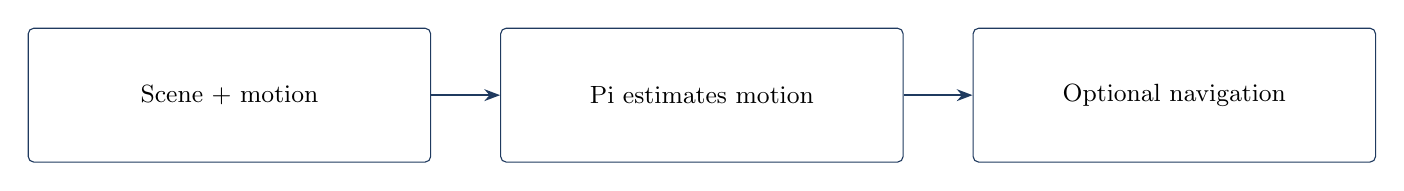
\begin{tikzpicture}\node[box,text width=49mm,minimum height=17mm] (a0) at (0.0,0) {Scene + motion};\node[box,text width=49mm,minimum height=17mm] (a1) at (6.0,0) {Pi estimates motion};\draw[flow] (a0.east)--(a1.west);\node[box,text width=49mm,minimum height=17mm] (a2) at (12.0,0) {Optional navigation};\draw[flow] (a1.east)--(a2.west);\end{tikzpicture}}{The separate STM32 balance path does not wait for this chain.}
\vfill\takeaway{Why WBR cares: a navigation aid must have a clear failure boundary.}
\note{base/main-v4-91p.tex; base/main.tex Phase 8; docs/PROJECT\_STATE.md and NEXT\_GATE.md. Offline teaching synthesis; no new physical evidence.}
\end{frame}
\begin{frame}{Research questions become experiments}
\evidence{SOURCE-SUPPORTED project objectives / results OPEN}
\deckitems{\item Can the Pi sustain the exact stream? Answer with counts, gaps and power logs, before SLAM.\item Does the same frozen take initialize repeatedly? Answer with all run and reset events.\item Is output useful and fresh? Answer with accuracy, continuity, age and receiver rejection tests.}
\vfill\takeaway{Write the question, measured quantity and rejection rule before a run.}
\note{base/main-v4-91p.tex; base/main.tex Phase 8; docs/PROJECT\_STATE.md and NEXT\_GATE.md. Offline teaching synthesis; no new physical evidence.}
\end{frame}
\begin{frame}{Sensor-to-pose: follow one image interval}
\evidence{KNOWN method / WBR qualification OPEN}
\deckitems{\item The SDK acquires sensor frames; the wrapper publishes typed ROS messages.\item A recorder preserves input. A reviewed adapter pairs stereo and attaches covered IMU samples.\item Tracking produces a state; its health and pose epoch must accompany any downstream use.}
\par\medskip \coursefigure{b2-execution}{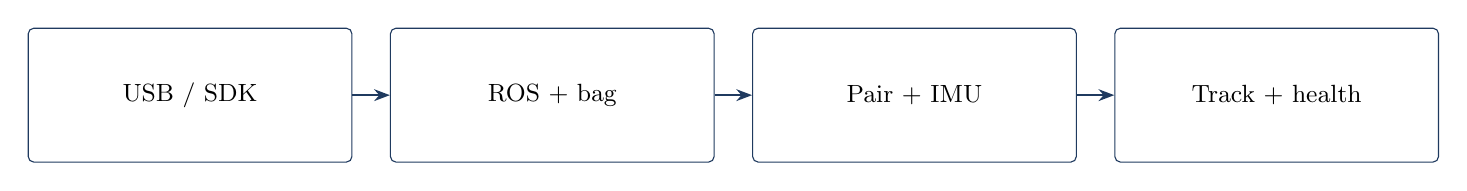
\begin{tikzpicture}\node[box,text width=39mm,minimum height=17mm] (a0) at (0.0,0) {USB / SDK};\node[box,text width=39mm,minimum height=17mm] (a1) at (4.6,0) {ROS + bag};\draw[flow] (a0.east)--(a1.west);\node[box,text width=39mm,minimum height=17mm] (a2) at (9.2,0) {Pair + IMU};\draw[flow] (a1.east)--(a2.west);\node[box,text width=39mm,minimum height=17mm] (a3) at (13.799999999999999,0) {Track + health};\draw[flow] (a2.east)--(a3.west);\end{tikzpicture}}{Planned ROS stereo path; current native recording is a separate branch.}
\vfill\takeaway{Why WBR cares: a fault at an earlier boundary contaminates every later claim.}
\note{base/main-v4-91p.tex; base/main.tex Phase 8; docs/PROJECT\_STATE.md and NEXT\_GATE.md. Offline teaching synthesis; no new physical evidence.}
\end{frame}
\begin{frame}{Machine ownership: Mac, Pi and STM32}
\evidence{KNOWN method / WBR qualification OPEN}
\deckitems{\item The Mac holds canonical sources and performs home analysis; preserve its existing work.\item The Pi records locally into a separate checksummed runtime and evidence directory.\item SSH carries commands and small evidence. It is not the live image transport for qualification.}
\vfill\takeaway{Record source, binary, library, settings and dirty-file hashes for each runtime.}
\note{base v4 §3.1; canonical AGENTS.md and architecture; no deployment performed.}
\end{frame}
\begin{frame}{Research design: check yourself}
\evidence{KNOWN method / illustrative question}
\deckitems{\item A run exits successfully but its pose is 400 ms old. Which research question remains unanswered?}
\vfill\takeaway{Work out your answer before turning the page.}
\note{base/main-v4-91p.tex; base/main.tex Phase 8; docs/PROJECT\_STATE.md and NEXT\_GATE.md. Offline teaching synthesis; no new physical evidence.}
\end{frame}
\begin{frame}{Research design: answer}
\evidence{KNOWN method / illustrative question}
\deckitems{\item Freshness remains unanswered. Exit status establishes process completion, not useful source age.\item A WBR receiver needs a bounded pose age and valid session/frame before using optional input.}
\vfill\takeaway{Explain the evidence that would distinguish the two cases.}
\note{base/main-v4-91p.tex; base/main.tex Phase 8; docs/PROJECT\_STATE.md and NEXT\_GATE.md. Offline teaching synthesis; no new physical evidence.}
\end{frame}
\begin{frame}{System ownership: why WBR needs two computers}
\evidence{KNOWN method}
\deckitems{\item The Pi runs perception and optional navigation on Linux.\item STM32H7 owns body estimation, balance and motor safety.\item LQR = Linear Quadratic Regulator; VMC = Virtual Model Control.\item The Nucleo-F446RE is a link/supervisor stand-in, not the WBR controller.}
\par\medskip \coursefigure{owners}{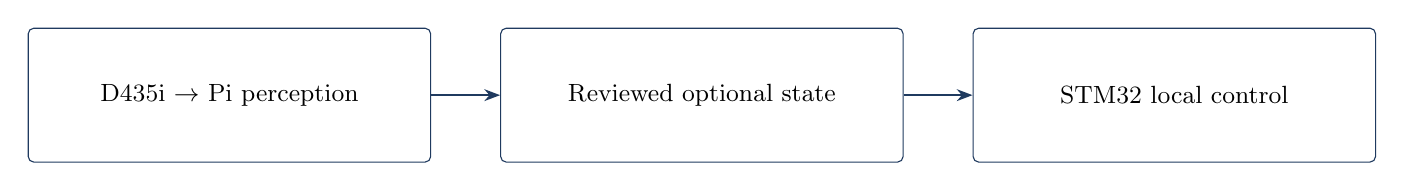
\begin{tikzpicture}\node[box,text width=49mm,minimum height=17mm] (a0) at (0.0,0) {D435i $\to$ Pi perception};\node[box,text width=49mm,minimum height=17mm] (a1) at (6.0,0) {Reviewed optional state};\draw[flow] (a0.east)--(a1.west);\node[box,text width=49mm,minimum height=17mm] (a2) at (12.0,0) {STM32 local control};\draw[flow] (a1.east)--(a2.west);\end{tikzpicture}}{Ownership boundary; no physical safety verdict.}
\vfill\takeaway{Pi loss must withdraw optional input while local control keeps authority.}
\note{Canonical AGENTS.md, docs/ARCHITECTURE.md, docs/DECISIONS.md ADR-001; WBR physical balance retention is untested.}
\end{frame}
\begin{frame}{Camera IMU and body IMU have different jobs}
\evidence{KNOWN method}
\deckitems{\item D435i inertial measurement unit (IMU) lives in imu\_camera.\item It supports visual-inertial odometry (VIO): motion from images and inertial data.\item The controller IMU lives in imu\_body and supports local balance.\item Different mounts, clocks and calibrations prohibit naive substitution.}
\vfill\takeaway{An IMU is a sensor type, not a shared reference frame.}
\note{Architecture ADR-002; camera and body IMUs remain separate.}
\end{frame}
\begin{frame}{Ownership: worked stale-input example}
\evidence{CALCULATED illustrative; no WBR age budget}
\deckitems{\item Illustrative: 20 ms inference is followed by 300 ms in a queue.\item Even a newly transmitted heartbeat can accompany a 320 ms old result.\item The receiver must assess source age, validity, frame and session.}
\par\medskip \[A=20+300=320\;\mathrm{ms}\]
\vfill\takeaway{Why WBR cares: fast arithmetic does not make a usable navigation input.}
\note{Study synthesis from base/main-v4-91p.tex, updated against base/main.tex. No new physical evidence; every gate remains OPEN.}
\end{frame}
\begin{frame}{Ownership: common mistake and check yourself}
\evidence{KNOWN method}
\deckitems{\item Mistake: reset the Linux process and assume its old pose is still valid.\item A new process/session may have a new origin, map and clock relation.\item Question: can the camera IMU replace the body IMU during Pi failure?}
\vfill\takeaway{Explain the independent control path aloud before connecting anything.}
\note{Answer: no. The camera path depends on the failed Pi and has unrelated mount/clock/calibration. STM32 retains its own sensing and safety authority.}
\end{frame}
\begin{frame}{Ownership: answer}
\evidence{KNOWN method / WBR qualification OPEN}
\deckitems{\item No. The camera path depends on the Pi and has unrelated mount, clock and calibration.\item STM32 keeps independent body sensing and local balance authority.}
\vfill\takeaway{Use this answer to check the reasoning on the preceding page.}
\note{base/main-v4-91p.tex; base/main.tex Phase 8; docs/PROJECT\_STATE.md and NEXT\_GATE.md. Offline teaching synthesis; no new physical evidence.}
\end{frame}
\begin{frame}{D435i inputs and the identity that matters}
\evidence{MEASURED archived identity / fresh readback OPEN}
\deckitems{\item New SDK serial 317422076650; firmware readback 5.17.3.10; BMI085.\item Keep SDK, ASIC, firmware-update and USB descriptor serial fields separate.\item Old SDK serial 243322073847 has no transferable gate receipts.}
\vfill\takeaway{Why WBR cares: a replacement camera needs fresh acquisition evidence.}
\note{base/main.tex Phase-8 D435i sensor inputs; docs/PROJECT\_STATE.md; canonical N1 runbook. ASIC/descriptor observed 327743061057; firmware-update ID must be freshly established.}
\end{frame}
\begin{frame}{Two stream profiles: never merge their evidence}
\evidence{SOURCE-SUPPORTED profiles / qualification OPEN}
\begin{tabular}{@{}L{57mm}L{76mm}L{47mm}@{}}\toprule
\textbf{Purpose} & \textbf{IR images} & \textbf{Raw motion}\\\midrule
N2 qualification & IR1 Y8 640$\times$480, 15 Hz & Gyro 200; accel 100 Hz\\[6pt]
N4 development / S / C & IR1 + IR2 Y8 640$\times$480, 30 Hz & Gyro 200; accel 100 Hz\\[6pt]
A Allan / I diagnostics & No images & Gyro 200; accel 100 Hz\\[6pt]\bottomrule\end{tabular}\vfill\takeaway{N2 still needs 20 $\to$ 105 $\to$ 300 s, including the 300-second soak.}
\note{Study synthesis from base/main-v4-91p.tex, updated against base/main.tex. No new physical evidence; every gate remains OPEN.}
\end{frame}
\begin{frame}{USB and power: inspect the camera branch}
\evidence{MEASURED historical / SOURCE-SUPPORTED requirement}
\deckitems{\item D435i goes directly to a blue USB 3 port with its own known cable.\item The camera node must show $\geq$5000M; a 5000M root hub is insufficient.\item The 8 GB Pi booted the old card, but historical under-voltage persisted.}
\vfill\takeaway{Why WBR cares: missing motion or frames can originate below the estimator.}
\note{base/main.tex current hardware and USB; docs/PROJECT\_STATE.md. CN HARDWARE.md later owner inventory reports one official 27 W PSU; arrival is not WBR qualification.}
\end{frame}
\begin{frame}{Power faults propagate into sensor symptoms}
\evidence{KNOWN method / WBR qualification OPEN}
\deckitems{\item A weak supply can produce resets, USB interruptions or throttling under acquisition load.\item Keep both current fault bits and historical sticky bits; a later clean sample does not erase a fault.\item A newly available 27 W supply still needs loaded evidence on this exact assembly.}
\par\medskip \coursefigure{b2-power}{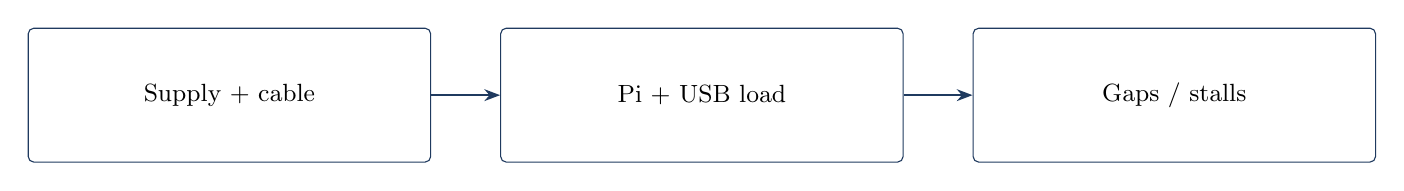
\begin{tikzpicture}\node[box,text width=49mm,minimum height=17mm] (a0) at (0.0,0) {Supply + cable};\node[box,text width=49mm,minimum height=17mm] (a1) at (6.0,0) {Pi + USB load};\draw[flow] (a0.east)--(a1.west);\node[box,text width=49mm,minimum height=17mm] (a2) at (12.0,0) {Gaps / stalls};\draw[flow] (a1.east)--(a2.west);\end{tikzpicture}}{Diagnostic causal possibilities, not a proven cause for every dropped frame.}
\vfill\takeaway{Check power before changing drivers or estimator settings.}
\note{base/main-v4-91p.tex; base/main.tex Phase 8; docs/PROJECT\_STATE.md and NEXT\_GATE.md. Offline teaching synthesis; no new physical evidence.}
\end{frame}
\begin{frame}{Storage: calculate the payload before recording}
\evidence{CALCULATED payload / MEASURED USB-stick rate}
\deckitems{\item Each Y8 image has 640$\times$480 bytes; two views arrive 30 times each second.\item The payload alone is 18.432 MB/s before serialization and indexes.\item Two 120 s representations can require over 4.4 GB, before derived files.}
\par\medskip \[2(640)(480)(30)=18{,}432{,}000\;\mathrm{B/s}\]
\vfill\takeaway{The 1.09 MB/s USB2 stick cannot record this stream.}
\note{Study synthesis from base/main-v4-91p.tex, updated against base/main.tex. No new physical evidence; every gate remains OPEN.}
\end{frame}
\begin{frame}{Storage qualification: identity and sustained writes}
\evidence{SOURCE-SUPPORTED contract / gate OPEN}
\begin{tabular}{@{}L{80mm}L{100mm}@{}}\toprule
\textbf{Check} & \textbf{What it proves}\\\midrule
Mount source + UUID + physical device & The output path reaches the intended data volume.\\[6pt]
Overall and worst fsync-batch rate & Cache bursts do not hide long durable-write stalls.\\[6pt]
SHA-256 readback + free-space reserve & Data survived the write and future takes have room.\\[6pt]\bottomrule\end{tabular}\vfill\takeaway{Why WBR cares: a fast sensor can be delayed by a slow recorder.}
\note{v4 §3.8 and §4.7; current calibration plan card exception; no write benchmark executed.}
\end{frame}
\begin{frame}{Storage: worked load and margin}
\evidence{MEASURED historical rate / CALCULATED deficit / ASSUMED margin}
\deckitems{\item The observed card rate was 16.6 MB/s; stereo image payload is about 18.4 MB/s.\item Illustrative deficit: (18.4 − 16.6) $\times$ 60 ≈ 108 MB accumulates in one minute.\item The approved card exception proposes $\geq$27.6 MB/s, a 1.5$\times$ margin, plus a take-length test.}
\par\medskip \[R_{write}<R_{in}\quad\Longrightarrow\quad\text{backlog grows until a buffer fills}\]
\vfill\takeaway{A higher card capacity does not establish sustained speed or a valid N3 receipt.}
\note{base/main-v4-91p.tex; base/main.tex Phase 8; docs/PROJECT\_STATE.md and NEXT\_GATE.md. Offline teaching synthesis; no new physical evidence.}
\end{frame}
\begin{frame}{Storage review: check yourself}
\evidence{KNOWN method / illustrative question}
\deckitems{\item Mistake: an empty mount directory exists, so a recording is on the external disk. What must you inspect?}
\vfill\takeaway{Work out your answer before turning the page.}
\note{base/main-v4-91p.tex; base/main.tex Phase 8; docs/PROJECT\_STATE.md and NEXT\_GATE.md. Offline teaching synthesis; no new physical evidence.}
\end{frame}
\begin{frame}{Storage review: answer}
\evidence{KNOWN method / illustrative question}
\deckitems{\item Inspect the resolved mount source, partition UUID and physical device, then the qualified write receipt.\item If the mount failed, the same path can resolve to the boot card. Stop before the bag is recorded.}
\vfill\takeaway{Explain the evidence that would distinguish the two cases.}
\note{base/main-v4-91p.tex; base/main.tex Phase 8; docs/PROJECT\_STATE.md and NEXT\_GATE.md. Offline teaching synthesis; no new physical evidence.}
\end{frame}
\begin{frame}{Hardware: common mistake and check yourself}
\evidence{KNOWN method}
\deckitems{\item Mistake: a larger RAM board repairs a weak supply or slow card.\item A 15 s RAM diagnostic had zero observed drops; long card writes were gapped.\item Question: does a clean RAM capture qualify persistent storage?}
\vfill\takeaway{Separate transport, temporary capture, durable copy and replay evidence.}
\note{Answer: no. Phase 8 reports 29.99 Hz IR, 33 ms maximum gap, gyro 200.2 and accel 101 Hz for the short RAM test. Card take had 0.3–2.9 s gaps after 22 s; writer blocking is INFERRED.}
\end{frame}
\begin{frame}{Hardware: answer}
\evidence{KNOWN method / WBR qualification OPEN}
\deckitems{\item No. A clean RAM capture checks a short acquisition window, not durable storage.\item The archived 15 s RAM test was clean; the longer card take had 0.3–2.9 s gaps after 22 s.}
\vfill\takeaway{Use this answer to check the reasoning on the preceding page.}
\note{base/main-v4-91p.tex; base/main.tex Phase 8; docs/PROJECT\_STATE.md and NEXT\_GATE.md. Offline teaching synthesis; no new physical evidence.}
\end{frame}
\begin{frame}{Stereo geometry: two views constrain depth}
\evidence{KNOWN method}
\deckitems{\item Rectification makes corresponding scene points lie on a shared image row.\item Disparity is left u minus right u; baseline is a positive distance.\item Wrong pairing, camera order or focal length makes metric depth wrong.}
\par\medskip \[d=u_L-u_R,\qquad Z=\frac{f_x b}{d}\]
\par\medskip \coursefigure{stereo}{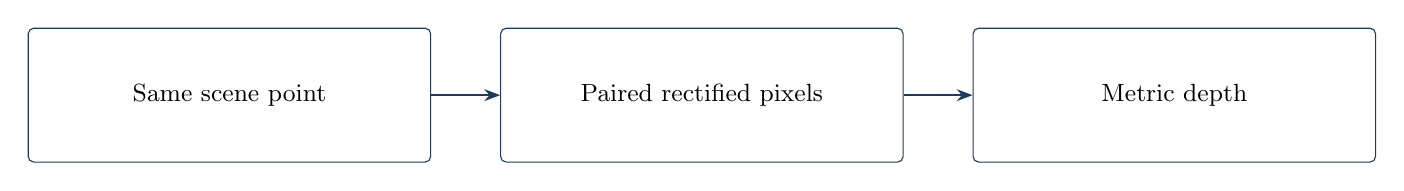
\begin{tikzpicture}\node[box,text width=49mm,minimum height=17mm] (a0) at (0.0,0) {Same scene point};\node[box,text width=49mm,minimum height=17mm] (a1) at (6.0,0) {Paired rectified pixels};\draw[flow] (a0.east)--(a1.west);\node[box,text width=49mm,minimum height=17mm] (a2) at (12.0,0) {Metric depth};\draw[flow] (a1.east)--(a2.west);\end{tikzpicture}}{Conceptual stereo reasoning, not a depth measurement.}
\vfill\takeaway{Why WBR cares: stereo gives scale only with valid geometry.}
\note{Study synthesis from base/main-v4-91p.tex, updated against base/main.tex. No new physical evidence; every gate remains OPEN.}
\end{frame}
\begin{frame}{Features connect stereo views and time}
\evidence{KNOWN method / WBR qualification OPEN}
\deckitems{\item A feature is a repeatable image location and descriptor, not a sensor measurement of pose.\item Stereo matches constrain depth at one epoch; temporal matches constrain motion between epochs.\item Reject ambiguous correspondences and inspect geometry before increasing feature count.}
\par\medskip \coursefigure{b2-feature}{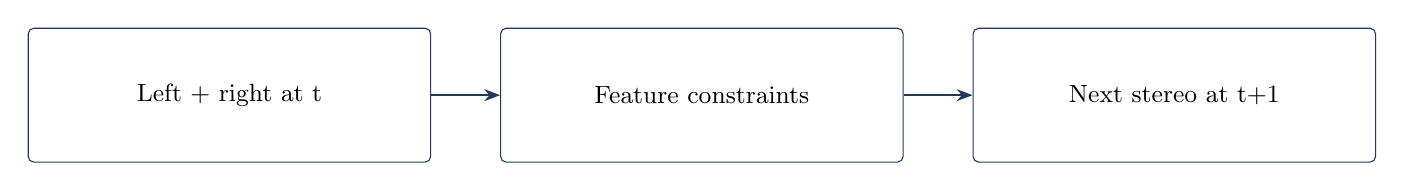
\begin{tikzpicture}\node[box,text width=49mm,minimum height=17mm] (a0) at (0.0,0) {Left + right at t};\node[box,text width=49mm,minimum height=17mm] (a1) at (6.0,0) {Feature constraints};\draw[flow] (a0.east)--(a1.west);\node[box,text width=49mm,minimum height=17mm] (a2) at (12.0,0) {Next stereo at t+1};\draw[flow] (a1.east)--(a2.west);\end{tikzpicture}}{Stereo and temporal constraints cooperate; neither guarantees a correct match.}
\vfill\takeaway{Why WBR cares: natural texture must remain observable while the robot moves.}
\note{base/main-v4-91p.tex; base/main.tex Phase 8; docs/PROJECT\_STATE.md and NEXT\_GATE.md. Offline teaching synthesis; no new physical evidence.}
\end{frame}
\begin{frame}{Emitter off: preserve the meaning of a feature}
\evidence{ASSUMED protocol / SOURCE-SUPPORTED rationale}
\deckitems{\item The projector adds infrared texture tied to the camera rather than fixed scene texture.\item For natural-feature tracking and target calibration, the plan selects emitter OFF.\item Use sufficient ambient near-infrared light. If the target is dark, improve light or print first.}
\vfill\takeaway{Log actual emitter and exposure readback; an intended setting is not observed behavior.}
\note{Phase-8 M4 projector-off explanation; current calibration plan target/light protocol.}
\end{frame}
\begin{frame}{Stereo: worked depth and disparity}
\evidence{MEASURED readback / CALCULATED example}
\deckitems{\item Factory readback: fx = 386.9533 px; baseline = 0.04991255 m.\item Their product is 19.31383 px·m; at 1 m the ideal disparity is 19.31 px.\item At disparity 10 px, calculated depth is about 1.931 m.}
\par\medskip \[f_x b=19.31383\;\mathrm{px\,m},\quad Z(10\;\mathrm{px})=1.93138\;\mathrm{m}\]
\vfill\takeaway{The calculation uses readback geometry; it is not independent accuracy.}
\note{docs/D435I\_CALIBRATION\_PLAN.md §1–2. Distances measured from left optical center, not housing front.}
\end{frame}
\begin{frame}{Stereo: small disparity makes distant depth fragile}
\evidence{CALCULATED first-order illustrative error}
\deckitems{\item Differentiate Z = fb/d: a small pixel error has increasing depth effect.\item At 2 m, d ≈ 9.657 px; illustrative 0.5 px error gives ≈0.104 m error.\item Lighting, blur, target visibility and stereo skew affect matching.}
\par\medskip \[|\delta Z|\approx\frac{Z^2}{f_xb}|\delta d|=\frac{4}{19.31383}(0.5)=0.104\;\mathrm{m}\]
\vfill\takeaway{Use static S intervals before diagnosing a geometric failure.}
\note{Study synthesis from base/main-v4-91p.tex, updated against base/main.tex. No new physical evidence; every gate remains OPEN.}
\end{frame}
\begin{frame}{Stereo: common mistake and check yourself}
\evidence{KNOWN method}
\deckitems{\item Mistake: copy the SDK negative x translation into Stereo.b.\item SDK IR1$\to$IR2 has tx = −b; ORB baseline magnitude is +b.\item Question: if left/right images are exchanged, what happens to disparity?}
\vfill\takeaway{Test frame direction and signs before changing feature thresholds.}
\note{Answer: disparity changes sign for the same ordering convention, producing negative inferred Z if the model is not changed. Stereo.T\_c1\_c2 is right$\to$left; Kalibr cam1.T\_cn\_cnm1 is left$\to$right.}
\end{frame}
\begin{frame}{Stereo: answer}
\evidence{KNOWN method / WBR qualification OPEN}
\deckitems{\item Exchanging left and right reverses disparity under the same convention.\item The unchanged formula then produces negative depth. Repair ordering and transform direction before tuning features.}
\vfill\takeaway{Use this answer to check the reasoning on the preceding page.}
\note{base/main-v4-91p.tex; base/main.tex Phase 8; docs/PROJECT\_STATE.md and NEXT\_GATE.md. Offline teaching synthesis; no new physical evidence.}
\end{frame}
\begin{frame}{IMU model: what the two channels measure}
\evidence{KNOWN method}
\deckitems{\item Gyro measures angular rate plus bias and noise, in rad/s.\item Accelerometer measures specific force, including the gravity relation.\item Bias, scale/misalignment, white noise and bias walk are different errors.}
\par\medskip \[\omega_m=\omega+b_g+n_g,\qquad a_m=R_{bw}(a_w-g_w)+b_a+n_a\]
\vfill\takeaway{Why WBR cares: systematic IMU errors bend prediction between images.}
\note{Pedagogical ideal model; all symbols frame-defined here. Separate physical scale/misalignment diagnostics are needed; no full intrinsic calibration is claimed.}
\end{frame}
\begin{frame}{IMU errors enter prediction before the next image}
\evidence{KNOWN method / WBR qualification OPEN}
\deckitems{\item Integrating angular rate predicts orientation; rotating specific force helps predict velocity.\item Bias is a systematic offset. White noise and bias walk describe different stochastic behavior.\item An incorrect frame or time interval can look like bad noise tuning.}
\par\medskip \coursefigure{b2-imu}{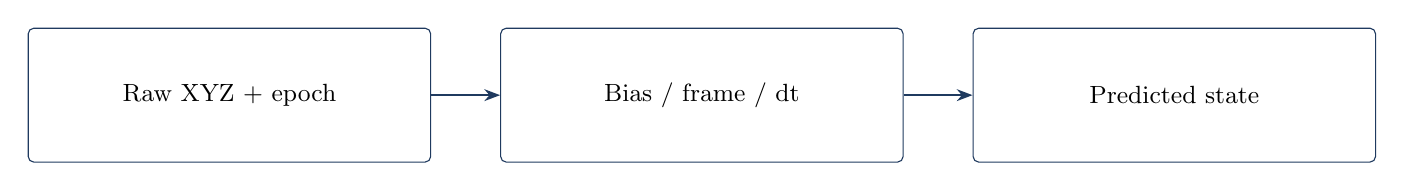
\begin{tikzpicture}\node[box,text width=49mm,minimum height=17mm] (a0) at (0.0,0) {Raw XYZ + epoch};\node[box,text width=49mm,minimum height=17mm] (a1) at (6.0,0) {Bias / frame / dt};\draw[flow] (a0.east)--(a1.west);\node[box,text width=49mm,minimum height=17mm] (a2) at (12.0,0) {Predicted state};\draw[flow] (a1.east)--(a2.west);\end{tikzpicture}}{Conceptual propagation; scale and misalignment are not corrected by this drawing.}
\vfill\takeaway{Why WBR cares: visual correction has to repair the prediction built from these inputs.}
\note{base/main-v4-91p.tex; base/main.tex Phase 8; docs/PROJECT\_STATE.md and NEXT\_GATE.md. Offline teaching synthesis; no new physical evidence.}
\end{frame}
\begin{frame}{Visual-inertial prediction bridges image intervals}
\evidence{KNOWN method}
\deckitems{\item At 30 Hz, image intervals are about 33.3 ms; gyro nominal dt is 5 ms.\item Gyro-grid association uses original gyro and bracketed interpolated accel.\item Visual residuals correct accumulated propagation errors.}
\par\medskip \coursefigure{vio}{
\begin{tikzpicture}\node[box,text width=49mm,minimum height=17mm] (a0) at (0.0,0) {IMU propagation};\node[box,text width=49mm,minimum height=17mm] (a1) at (6.0,0) {Image constraints};\draw[flow] (a0.east)--(a1.west);\node[box,text width=49mm,minimum height=17mm] (a2) at (12.0,0) {Corrected state};\draw[flow] (a1.east)--(a2.west);\end{tikzpicture}}{Timing and geometry must connect both sensor cues.}
\vfill\takeaway{Interpolation adds an aligned input grid, not a new sensor.}
\note{Study synthesis from base/main-v4-91p.tex, updated against base/main.tex. No new physical evidence; every gate remains OPEN.}
\end{frame}
\begin{frame}{IMU: worked bias and noise scaling}
\evidence{CALCULATED illustrative / ASSUMED candidate noise}
\deckitems{\item Illustrative uncorrected gyro bias 0.01 rad/s accumulates 0.1 rad in 10 s.\item That is about 5.73$^\circ$ before visual correction; it is not this unit’s bias.\item Continuous gyro density 0.001 at 200 Hz gives discrete $\sigma$ ≈ 0.01414 rad/s.}
\par\medskip \[\delta\theta=b_gT=0.1\;\mathrm{rad},\quad \sigma_d=N\sqrt{f}=0.001\sqrt{200}\]
\vfill\takeaway{ORB scales continuous densities internally; never discretize twice.}
\note{Study synthesis from base/main-v4-91p.tex, updated against base/main.tex. No new physical evidence; every gate remains OPEN.}
\end{frame}
\begin{frame}{Allan deviation: choose the supported region}
\evidence{KNOWN method}
\deckitems{\item Average stationary samples over $\tau$ and compare neighboring averages.\item A −1/2 log slope supports white-noise density N at $\tau$ = 1 s.\item A +1/2 slope supports walk K via its fitted value at $\tau$ = 3 s.}
\par\medskip \[\sigma_A^2(\tau)=\tfrac12\,\operatorname{mean}(\bar x_{k+m}-\bar x_k)^2\]
\vfill\takeaway{A flat bias-instability minimum is not the bias-walk coefficient.}
\note{docs/D435I\_CALIBRATION\_PLAN.md §5; calibration/allan/README.md. At least one decade, slope tolerance $\pm$0.1, fit R$^2$$\geq$0.95 and cluster support are ASSUMED tool review criteria.}
\end{frame}
\begin{frame}{Allan plot: read slopes, not just the minimum}
\evidence{CALCULATED schematic / unit noise UNKNOWN}
\deckitems{
\item A log-log slope identifies a candidate noise process over a supported range.
\item A short record has few independent long-$\tau$ clusters; the last points can mislead.}
\par\medskip
\coursefigure{b2-allan}{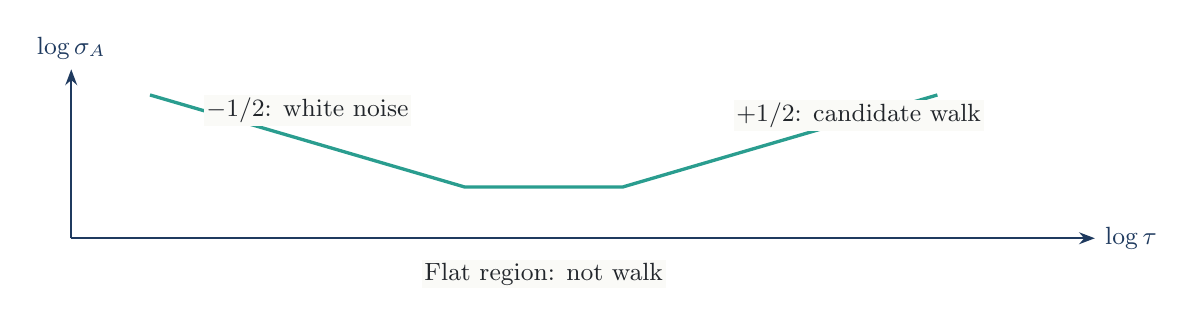
\begin{tikzpicture}[x=1cm,y=.65cm]
\draw[flow] (0,0)--(13,0) node[right]{\small $\log\tau$};
\draw[flow] (0,0)--(0,3.3) node[above]{\small $\log\sigma_A$};
\draw[teal,very thick] (1,2.8)--(5,1.0)--(7,1.0)--(11,2.8);
\node[lbl] at (3,2.5){$-1/2$: white noise};
\node[lbl] at (6,-.7){Flat region: not walk};
\node[lbl] at (10,2.4){$+1/2$: candidate walk};
\end{tikzpicture}}{Illustrative shape; no unit-specific Allan data are plotted.}
\vfill\takeaway{A fit needs enough clusters and a stable range, not a convenient slope.}
\note{Calibration plan §5 and calibration/allan/README.md. Sketch is illustrative, not a measured curve.}
\end{frame}
\begin{frame}{Allan: common mistake and check yourself}
\evidence{KNOWN method}
\deckitems{\item Mistake: use rounded vendor CSV or interpolated 200 Hz accel as raw data.\item Preserve XYZ full precision; raw accel remains 100 Hz and gyro 200 Hz.\item Question: can a clean 36 s pilot establish long-term random walk?}
\vfill\takeaway{Use the pilot for acquisition; plan $\geq$4 h provisional, preferably 15–24 h.}
\note{Answer: no. Short data may support timing checks or limited white-noise evidence, but not a supported long-$\tau$ walk. Report K UNKNOWN when the rising fit lacks support. Warm up 30 minutes and keep temperature/stationarity documented.}
\end{frame}
\begin{frame}{Allan: answer}
\evidence{KNOWN method / WBR qualification OPEN}
\deckitems{\item No. A 36 s pilot checks acquisition and some short-time behavior, not supported long-term walk.\item Use $\geq$4 h provisionally, preferably 15–24 h; report unsupported walk as UNKNOWN.}
\vfill\takeaway{Use this answer to check the reasoning on the preceding page.}
\note{base/main-v4-91p.tex; base/main.tex Phase 8; docs/PROJECT\_STATE.md and NEXT\_GATE.md. Offline teaching synthesis; no new physical evidence.}
\end{frame}
\begin{frame}{Frames: axes and the pose origin}
\evidence{KNOWN method}
\deckitems{\item Body convention: x forward, y left, z up. Optical: x right, y down, z forward.\item A trajectory describes a named sensor origin in a named reference frame.\item The camera-to-robot mount must be composed to obtain robot-body pose.}
\vfill\takeaway{Why WBR cares: a good camera trajectory can still give the wrong body motion.}
\note{base/main-v4-91p.tex frame definitions and Phase-8 pose origin; actual WBR mount is UNKNOWN.}
\end{frame}
\begin{frame}{Odometry and mapping answer different questions}
\evidence{KNOWN method / WBR qualification OPEN}
\deckitems{\item Odometry tracks locally continuous motion, although its accumulated drift may grow.\item Mapping reuses places to improve global consistency; a loop correction can move the map pose.\item Why WBR cares: feeding that jump into a continuous local reference can create an artificial command.}
\par\medskip \coursefigure{b2-odom}{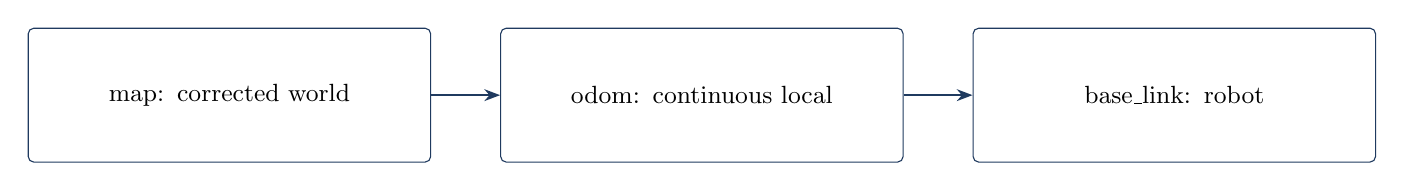
\begin{tikzpicture}\node[box,text width=49mm,minimum height=17mm] (a0) at (0.0,0) {map: corrected world};\node[box,text width=49mm,minimum height=17mm] (a1) at (6.0,0) {odom: continuous local};\draw[flow] (a0.east)--(a1.west);\node[box,text width=49mm,minimum height=17mm] (a2) at (12.0,0) {base\_link: robot};\draw[flow] (a1.east)--(a2.west);\end{tikzpicture}}{Planned transform semantics, not an implemented WBR continuity bridge.}
\vfill\takeaway{The map-to-odom continuity bridge needs its own explicit owner.}
\note{base/main-v4-91p.tex; base/main.tex Phase 8; docs/PROJECT\_STATE.md and NEXT\_GATE.md. Offline teaching synthesis; no new physical evidence.}
\end{frame}
\begin{frame}{Robot transforms: assign each edge an owner}
\evidence{KNOWN method / WBR qualification OPEN}
\deckitems{\item The robot description owns static mounts such as base\_link to camera\_link and body IMU.\item A future estimator/continuity bridge must explicitly own dynamic map, odom and body edges.\item An external world reference is optional and needs its own documented source.}
\par\medskip \coursefigure{b2-robot-tf}{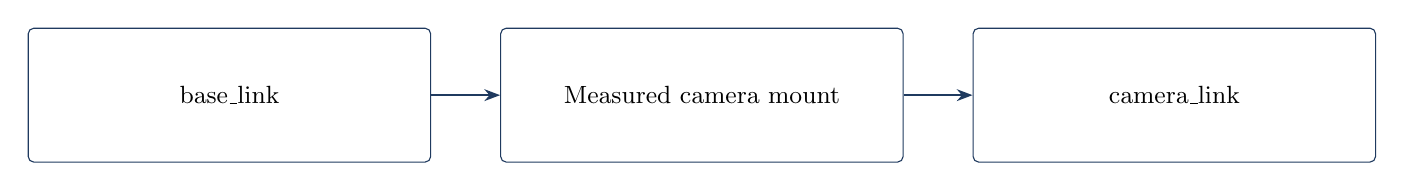
\begin{tikzpicture}\node[box,text width=49mm,minimum height=17mm] (a0) at (0.0,0) {base\_link};\node[box,text width=49mm,minimum height=17mm] (a1) at (6.0,0) {Measured camera mount};\draw[flow] (a0.east)--(a1.west);\node[box,text width=49mm,minimum height=17mm] (a2) at (12.0,0) {camera\_link};\draw[flow] (a1.east)--(a2.west);\end{tikzpicture}}{Static robot mount is separate from dynamic pose estimation.}
\vfill\takeaway{One child frame has one parent and one publisher.}
\note{base/main-v4-91p.tex; base/main.tex Phase 8; docs/PROJECT\_STATE.md and NEXT\_GATE.md. Offline teaching synthesis; no new physical evidence.}
\end{frame}
\begin{frame}{Camera transforms: inspect the wrapper tree}
\evidence{KNOWN method / WBR qualification OPEN}
\deckitems{\item The RealSense wrapper owns its internal optical and motion-sensor geometry.\item With tf\_publish\_rate = 0, inspect its static TF and the actual frame IDs.\item The camera-to-body mount remains a separate robot measurement; camera factory data do not supply it.}
\par\medskip \coursefigure{b2-camera-tf}{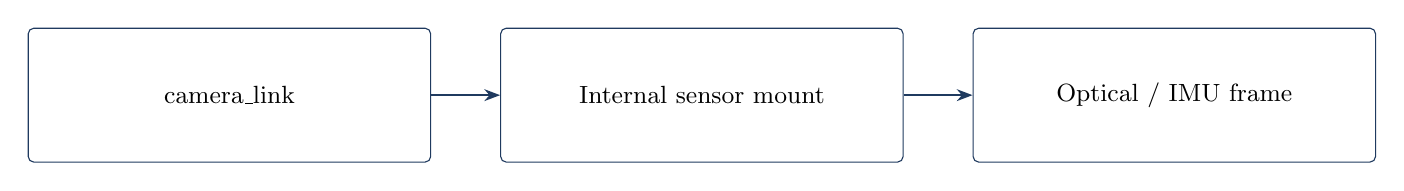
\begin{tikzpicture}\node[box,text width=49mm,minimum height=17mm] (a0) at (0.0,0) {camera\_link};\node[box,text width=49mm,minimum height=17mm] (a1) at (6.0,0) {Internal sensor mount};\draw[flow] (a0.east)--(a1.west);\node[box,text width=49mm,minimum height=17mm] (a2) at (12.0,0) {Optical / IMU frame};\draw[flow] (a1.east)--(a2.west);\end{tikzpicture}}{Conceptual wrapper-owned edge; actual names must come from the observed graph.}
\vfill\takeaway{Do not publish a copied conceptual sensor tree on top of the wrapper.}
\note{base/main-v4-91p.tex; base/main.tex Phase 8; docs/PROJECT\_STATE.md and NEXT\_GATE.md. Offline teaching synthesis; no new physical evidence.}
\end{frame}
\begin{frame}{Mapping continuity: check yourself}
\evidence{CALCULATED illustrative / bridge OPEN}
\deckitems{\item Worked case: loop correction moves map pose by 0.20 m while the robot is stationary. Did the robot move?}
\vfill\takeaway{Work out your answer before turning the page.}
\note{base/main-v4-91p.tex; base/main.tex Phase 8; docs/PROJECT\_STATE.md and NEXT\_GATE.md. Offline teaching synthesis; no new physical evidence.}
\end{frame}
\begin{frame}{Mapping continuity: answer}
\evidence{CALCULATED illustrative / bridge OPEN}
\deckitems{\item No. The reference estimate changed. A 0.20 m map correction is not evidence of physical body motion.\item The common mistake is to relabel map pose as continuous odom without maintaining the transform between them.}
\vfill\takeaway{Explain the evidence that would distinguish the two cases.}
\note{base/main-v4-91p.tex; base/main.tex Phase 8; docs/PROJECT\_STATE.md and NEXT\_GATE.md. Offline teaching synthesis; no new physical evidence.}
\end{frame}
\begin{frame}{Transforms: write the direction as an equation}
\evidence{KNOWN method}
\deckitems{\item T\_ab maps coordinates from b into a: p\_a = R\_ab p\_b + t\_ab.\item The inverse rotation is transpose; inverse translation is −R$^{T}$t.\item Keep mathematical rotation direction separate from array storage order.}
\par\medskip \[T_{ab}^{-1}=\begin{bmatrix}R_{ab}^{T}&-R_{ab}^{T}t_{ab}\\0&1\end{bmatrix}\]
\vfill\takeaway{A name such as Tbc is useful only with its mapping equation.}
\note{Study synthesis from base/main-v4-91p.tex, updated against base/main.tex. No new physical evidence; every gate remains OPEN.}
\end{frame}
\begin{frame}{Transforms: worked rotated lever arm}
\evidence{CALCULATED illustrative}
\deckitems{\item Illustrative camera origin is 0.1 m along the body x axis.\item A 90$^\circ$ body yaw rotates that lever arm into the world y axis.\item Copying camera position to base\_link creates orientation-dependent error.}
\par\medskip \[R_z(90^\circ)\begin{bmatrix}0.1\\0\\0\end{bmatrix}=\begin{bmatrix}0\\0.1\\0\end{bmatrix}\]
\vfill\takeaway{Rigid alignment cannot remove a changing lever-arm error.}
\note{Study synthesis from base/main-v4-91p.tex, updated against base/main.tex. No new physical evidence; every gate remains OPEN.}
\end{frame}
\begin{frame}{Frames: common mistake and check yourself}
\evidence{KNOWN method}
\deckitems{\item Mistake: publish the same TF child from both wrapper and robot description.\item Wrapper owns internal sensor geometry; robot description owns its mount.\item Question: can a loop-corrected map pose be relabeled continuous odom?}
\vfill\takeaway{Assign one parent and one publisher per child.}
\note{Answer: no. Loop correction may jump map pose. A continuity owner must explicitly maintain map$\to$odom and continuous odom$\to$base semantics; that bridge is not established by current WBR code.}
\end{frame}
\begin{frame}{Frames: answer}
\evidence{KNOWN method / WBR qualification OPEN}
\deckitems{\item No. A loop-corrected map pose can jump, whereas odom promises local continuity.\item An explicit owner must maintain map-to-odom and body-mount semantics; that bridge remains OPEN.}
\vfill\takeaway{Use this answer to check the reasoning on the preceding page.}
\note{base/main-v4-91p.tex; base/main.tex Phase 8; docs/PROJECT\_STATE.md and NEXT\_GATE.md. Offline teaching synthesis; no new physical evidence.}
\end{frame}
\begin{frame}{Timestamp chain: every kind has an owner}
\evidence{KNOWN method}
\begin{tabular}{@{}L{64mm}L{116mm}@{}}\toprule
\textbf{Stamp} & \textbf{Owner / meaning}\\\midrule
Physical capture & Actual exposure/measurement event; convention UNKNOWN.\\[6pt]
Device / SDK frame & Hardware, global or system domain; keep raw metadata.\\[6pt]
Driver / ROS header & Wrapper assigns the message’s source epoch.\\[6pt]
Publish / subscriber receipt & Different events; instrument on a stated host clock.\\[6pt]\bottomrule\end{tabular}\vfill\takeaway{A shared unit such as nanoseconds does not imply a shared clock.}
\note{Study synthesis from base/main-v4-91p.tex, updated against base/main.tex. No new physical evidence; every gate remains OPEN.}
\end{frame}
\begin{frame}{Timestamp chain: processing, bag and output}
\evidence{KNOWN method}
\begin{tabular}{@{}L{68mm}L{112mm}@{}}\toprule
\textbf{Stamp} & \textbf{Meaning}\\\midrule
Processing start / end & Local queue wait and compute intervals.\\[6pt]
ROS bag storage time & Recorder event; never a substitute for header/capture.\\[6pt]
Estimator pose epoch & Time the estimated state describes.\\[6pt]
Emission / file write / MCU receipt & Availability and receiver events, not pose epochs.\\[6pt]\bottomrule\end{tabular}\vfill\takeaway{Why WBR cares: measuring compute alone misses old input and queueing.}
\note{Study synthesis from base/main-v4-91p.tex, updated against base/main.tex. No new physical evidence; every gate remains OPEN.}
\end{frame}
\begin{frame}{Clocks: worked same-clock latency}
\evidence{CALCULATED illustrative}
\deckitems{\item Illustrative host-steady events: receive 10, start 30, end 42, emit 45 ms.\item Queue = 20 ms; compute = 12 ms; emission overhead = 3 ms.\item Receipt-to-output = 35 ms; physical capture age is still UNKNOWN.}
\par\medskip \[L_{rx\to o}=(30-10)+(42-30)+(45-42)=35\;\mathrm{ms}\]
\vfill\takeaway{Capture age also needs a measured mapping and uncertainty.}
\note{Study synthesis from base/main-v4-91p.tex, updated against base/main.tex. No new physical evidence; every gate remains OPEN.}
\end{frame}
\begin{frame}{Global time maps a clock; it does not measure exposure}
\evidence{KNOWN method / WBR qualification OPEN}
\deckitems{\item The SDK global-time option maps device timestamps toward host time.\item Save option readback and each frame domain. A configuration flag does not measure mapping error.\item Arrival minus mapped stamp includes mapping error and sensor/driver delay; it is not pure USB latency.}
\par\medskip \coursefigure{b2-global}{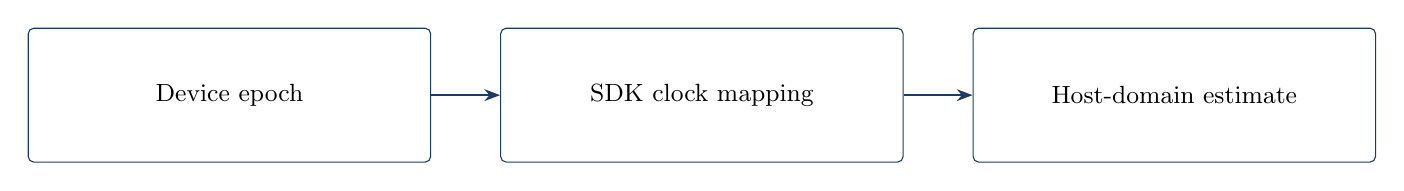
\begin{tikzpicture}\node[box,text width=49mm,minimum height=17mm] (a0) at (0.0,0) {Device epoch};\node[box,text width=49mm,minimum height=17mm] (a1) at (6.0,0) {SDK clock mapping};\draw[flow] (a0.east)--(a1.west);\node[box,text width=49mm,minimum height=17mm] (a2) at (12.0,0) {Host-domain estimate};\draw[flow] (a1.east)--(a2.west);\end{tikzpicture}}{Camera–IMU physical offset is a separate calibration question.}
\vfill\takeaway{Why WBR cares: usable age needs a clock relation and a stated uncertainty.}
\note{base/main-v4-91p.tex; base/main.tex Phase 8; docs/PROJECT\_STATE.md and NEXT\_GATE.md. Offline teaching synthesis; no new physical evidence.}
\end{frame}
\begin{frame}{Latency decomposition: put boundaries on the drawing}
\evidence{CALCULATED illustrative / capture age UNKNOWN}
\deckitems{\item Receipt, start, end and output use one host steady clock in this example.\item Queue wait Q, compute C and emission E add to receipt-to-output latency.\item Capture-to-receipt remains outside this interval until the device-to-host mapping is validated.}
\par\medskip \coursefigure{b2-latency}{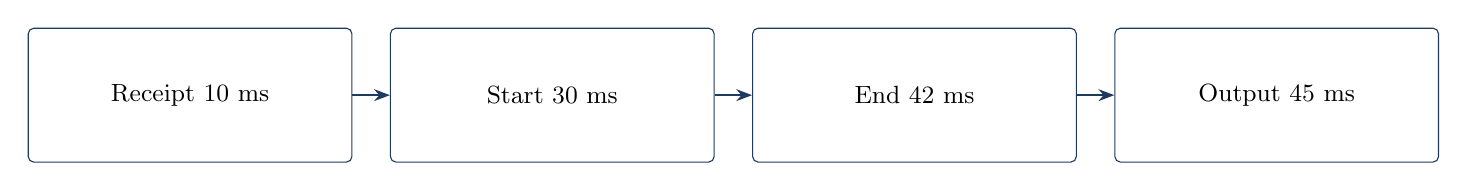
\begin{tikzpicture}\node[box,text width=39mm,minimum height=17mm] (a0) at (0.0,0) {Receipt 10 ms};\node[box,text width=39mm,minimum height=17mm] (a1) at (4.6,0) {Start 30 ms};\draw[flow] (a0.east)--(a1.west);\node[box,text width=39mm,minimum height=17mm] (a2) at (9.2,0) {End 42 ms};\draw[flow] (a1.east)--(a2.west);\node[box,text width=39mm,minimum height=17mm] (a3) at (13.799999999999999,0) {Output 45 ms};\draw[flow] (a2.east)--(a3.west);\end{tikzpicture}}{CALCULATED example: Q=20 ms, C=12 ms, E=3 ms; total 35 ms.}
\vfill\takeaway{A faster compute stage cannot remove a long wait that occurred before it.}
\note{base/main-v4-91p.tex; base/main.tex Phase 8; docs/PROJECT\_STATE.md and NEXT\_GATE.md. Offline teaching synthesis; no new physical evidence.}
\end{frame}
\begin{frame}{Age uncertainty: worked conservative bound}
\evidence{CALCULATED illustrative / WBR budget UNKNOWN}
\deckitems{\item Illustrative mapped capture time is 100 ms, output is 140 ms, mapping error is $\pm$3 ms.\item Estimated age is 40 ms; the supported age interval is 37–43 ms.\item If an illustrative receiver limit were 42 ms, the upper bound would not establish freshness.}
\par\medskip \[A\in[t_o-\widehat t_c-u,\ t_o-\widehat t_c+u]=[37,43]\;\mathrm{ms}\]
\vfill\takeaway{Use the conservative upper bound; the actual WBR age limit remains UNKNOWN.}
\note{base/main-v4-91p.tex; base/main.tex Phase 8; docs/PROJECT\_STATE.md and NEXT\_GATE.md. Offline teaching synthesis; no new physical evidence.}
\end{frame}
\begin{frame}{Clocks: common mistake and check yourself}
\evidence{KNOWN method}
\deckitems{\item Mistake: subtract an MCU timer from a Pi monotonic timestamp.\item Global-time enabled is configuration, not measured physical synchronization.\item Question: all streams say SYSTEM\_TIME; is equal-domain checking enough?}
\vfill\takeaway{Calibration rejects SYSTEM\_TIME even when every stream agrees.}
\note{Answer: no. Current calibration plan requires GLOBAL\_TIME or HARDWARE\_CLOCK plus supported metadata. SYSTEM\_TIME may be host-arrival fallback. Equality is necessary but does not establish exposure timing or intersensor offset.}
\end{frame}
\begin{frame}{Clocks: answer}
\evidence{KNOWN method / WBR qualification OPEN}
\deckitems{\item No. Equal SYSTEM\_TIME domains can still be host-arrival fallback.\item Calibration requires GLOBAL\_TIME or HARDWARE\_CLOCK plus supported metadata, not just equal domain names.}
\vfill\takeaway{Use this answer to check the reasoning on the preceding page.}
\note{base/main-v4-91p.tex; base/main.tex Phase 8; docs/PROJECT\_STATE.md and NEXT\_GATE.md. Offline teaching synthesis; no new physical evidence.}
\end{frame}
\begin{frame}{ROS 2: graph, typed topics and QoS}
\evidence{KNOWN method}
\deckitems{\item Robot Operating System 2 (ROS 2) connects typed publishers and subscribers.\item Data Distribution Service (DDS) provides transport and Quality of Service (QoS).\item QoS does not validate frames or clocks; isolate wrapper faults from the algorithm.}
\par\medskip \coursefigure{ros}{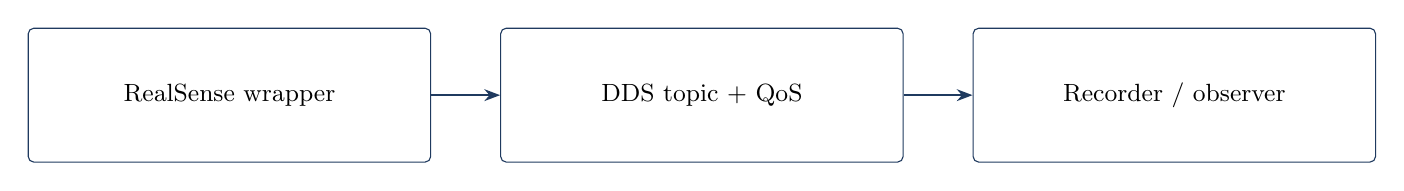
\begin{tikzpicture}\node[box,text width=49mm,minimum height=17mm] (a0) at (0.0,0) {RealSense wrapper};\node[box,text width=49mm,minimum height=17mm] (a1) at (6.0,0) {DDS topic + QoS};\draw[flow] (a0.east)--(a1.west);\node[box,text width=49mm,minimum height=17mm] (a2) at (12.0,0) {Recorder / observer};\draw[flow] (a1.east)--(a2.west);\end{tikzpicture}}{Planned WBR integration; native SDK diagnostics are separate.}
\vfill\takeaway{Inspect graph, type, QoS and payload together.}
\note{Study synthesis from base/main-v4-91p.tex, updated against base/main.tex. No new physical evidence; every gate remains OPEN.}
\end{frame}
\begin{frame}{QoS: compatibility before counting frames}
\evidence{KNOWN method}
\begin{tabular}{@{}L{65mm}L{80mm}L{35mm}@{}}\toprule
\textbf{Writer} & \textbf{Reader} & \textbf{Match?}\\\midrule
Best effort & Reliable & No\\[6pt]
Reliable & Best effort & Yes\\[6pt]
Volatile & Transient local & No\\[6pt]
Reliable + transient local & Same policy for static TF & Yes\\[6pt]\bottomrule\end{tabular}\vfill\takeaway{Use sensor-compatible QoS and durable static context.}
\note{Study synthesis from base/main-v4-91p.tex, updated against base/main.tex. No new physical evidence; every gate remains OPEN.}
\end{frame}
\begin{frame}{ROS topics: explicit sensor names}
\evidence{SOURCE-SUPPORTED names / observed graph OPEN}
\begin{tabular}{@{}L{102mm}L{78mm}@{}}\toprule
\textbf{Under /camera/camera/} & \textbf{Type / requested rate}\\\midrule
infra1/image\_rect\_raw; infra2/image\_rect\_raw & Image, 30 Hz each for stereo\\[6pt]
infra1/camera\_info; infra2/camera\_info & CameraInfo, matching image profile\\[6pt]
gyro/sample; accel/sample & Imu, raw 200 / 100 Hz\\[6pt]
/tf\_static (absolute) & TFMessage, reliable / transient local\\[6pt]\bottomrule\end{tabular}\vfill\takeaway{N3 baseline selects IR1/15 and extra context; IR2 needs separate attestation.}
\note{Study synthesis from base/main-v4-91p.tex, updated against base/main.tex. No new physical evidence; every gate remains OPEN.}
\end{frame}
\begin{frame}{Topic types are part of the input contract}
\evidence{SOURCE-SUPPORTED contract / gate OPEN}
\begin{tabular}{@{}L{83mm}L{97mm}@{}}\toprule
\textbf{ROS 2 type} & \textbf{What to inspect}\\\midrule
sensor\_msgs/msg/Image & Encoding, width/height, step, frame ID and original header.\\[6pt]
sensor\_msgs/msg/CameraInfo & Projection/model for that image profile and matching frame.\\[6pt]
sensor\_msgs/msg/Imu & Raw SI units; gyro and accel are separate sample topics.\\[6pt]
tf2\_msgs/msg/TFMessage & Static parents/children and durable /tf\_static delivery.\\[6pt]\bottomrule\end{tabular}\vfill\takeaway{Topic names alone cannot prove compatible contents.}
\note{base/main-v4-91p.tex; base/main.tex Phase 8; docs/PROJECT\_STATE.md and NEXT\_GATE.md. Offline teaching synthesis; no new physical evidence.}
\end{frame}
\begin{frame}{ROS bags: a durable record is an experiment input}
\evidence{KNOWN method}
\deckitems{\item Choose sqlite3 storage, explicit topics and a fresh take directory.\item Stop with Ctrl-C; wait for metadata finalization before hashing or copying.\item Retain parameter readback, wrapper log, QoS, metadata and power samples.}
\vfill\takeaway{Record in the lab; keep interpretation reproducible at home.}
\note{Study synthesis from base/main-v4-91p.tex, updated against base/main.tex. No new physical evidence; every gate remains OPEN.}
\end{frame}
\begin{frame}{ROS: worked queue and common mistake}
\evidence{CALCULATED illustrative / KNOWN ROS semantics}
\deckitems{\item At 30 Hz, ten queued images can add about 333 ms before processing.\item Mistake: ros2 topic hz looks nominal, so the bag must be complete.\item Question: can a late-starting volatile reader recover prior static TF?}
\par\medskip \[10/30=0.333\;\mathrm{s}\]
\vfill\takeaway{Compare counts, source stamps and context; do not infer them from rate.}
\note{Answer: a volatile reader does not request retained historical delivery. Use reliable/transient-local for /tf\_static, verify actual offer and record context. Nominal surviving-span rate can coexist with startup/tail losses.}
\end{frame}
\begin{frame}{ROS: answer}
\evidence{KNOWN method / WBR qualification OPEN}
\deckitems{\item A nominal ros2 topic hz observation does not prove the recorder stored every sample.\item Reconcile expected, received, stored and replayed counts, original headers, payloads and complete-window gaps.}
\vfill\takeaway{Use this answer to check the reasoning on the preceding page.}
\note{base/main-v4-91p.tex; base/main.tex Phase 8; docs/PROJECT\_STATE.md and NEXT\_GATE.md. Offline teaching synthesis; no new physical evidence.}
\end{frame}
\begin{frame}{Queues and backpressure: name every buffer}
\evidence{KNOWN method / WBR qualification OPEN}
\deckitems{\item The SDK, DDS transport, executor, recorder and estimator can each hold data.\item A full queue may block its producer or discard samples; record which policy applies.\item Record arrival/dequeue times, queue depth and discard reason. An unavailable counter is UNKNOWN.}
\par\medskip \coursefigure{b2-queue}{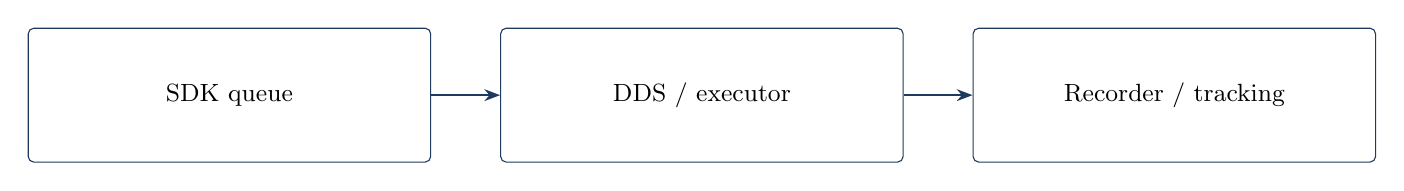
\begin{tikzpicture}\node[box,text width=49mm,minimum height=17mm] (a0) at (0.0,0) {SDK queue};\node[box,text width=49mm,minimum height=17mm] (a1) at (6.0,0) {DDS / executor};\draw[flow] (a0.east)--(a1.west);\node[box,text width=49mm,minimum height=17mm] (a2) at (12.0,0) {Recorder / tracking};\draw[flow] (a1.east)--(a2.west);\end{tikzpicture}}{Tracking runs on its caller; mapping and loop workers are separate scheduling loads.}
\vfill\takeaway{Why WBR cares: intact delivery can still be too old for navigation.}
\note{base/main-v4-91p.tex; base/main.tex Phase 8; docs/PROJECT\_STATE.md and NEXT\_GATE.md. Offline teaching synthesis; no new physical evidence.}
\end{frame}
\begin{frame}{Backpressure: worked overload}
\evidence{CALCULATED illustrative / actual queue policy OPEN}
\deckitems{\item Illustrative input is 30 images/s and service is 25 images/s: backlog grows by 5 each second.\item After 2 s, 10 queued images need about 400 ms of service before a new image is reached.\item A latest-only policy changes loss and continuity; it is not automatically valid for inertial tracking.}
\par\medskip \[\Delta q=(30-25)\cdot2=10,\qquad W\approx10/25=0.4\;\mathrm{s}\]
\vfill\takeaway{Bound queues and preserve image/IMU coverage; report discarded intervals.}
\note{base/main-v4-91p.tex; base/main.tex Phase 8; docs/PROJECT\_STATE.md and NEXT\_GATE.md. Offline teaching synthesis; no new physical evidence.}
\end{frame}
\begin{frame}{Queue diagnosis: check yourself}
\evidence{KNOWN method / illustrative question}
\deckitems{\item Mistake: deeper DDS history fixes a recorder that writes too slowly. What happens during sustained overload?}
\vfill\takeaway{Work out your answer before turning the page.}
\note{base/main-v4-91p.tex; base/main.tex Phase 8; docs/PROJECT\_STATE.md and NEXT\_GATE.md. Offline teaching synthesis; no new physical evidence.}
\end{frame}
\begin{frame}{Queue diagnosis: answer}
\evidence{KNOWN method / illustrative question}
\deckitems{\item The backlog still grows until the larger buffer fills, and waiting time can become worse.\item First compare durable write rate and input rate; preserve loss and queue evidence instead of changing several buffers.}
\vfill\takeaway{Explain the evidence that would distinguish the two cases.}
\note{base/main-v4-91p.tex; base/main.tex Phase 8; docs/PROJECT\_STATE.md and NEXT\_GATE.md. Offline teaching synthesis; no new physical evidence.}
\end{frame}
\begin{frame}{Calibration: four questions, four evidence types}
\evidence{KNOWN method}
\begin{tabular}{@{}L{75mm}L{105mm}@{}}\toprule
\textbf{Quantity} & \textbf{Current state}\\\midrule
Image intrinsics + stereo geometry & MEASURED factory readback; optical validation OPEN.\\[6pt]
Camera–IMU extrinsic & INFERRED nominal CAD; unit alignment OPEN.\\[6pt]
Camera–IMU time offset & UNKNOWN; zero is an operating assumption.\\[6pt]
IMU densities / walks & ASSUMED example values; unit Allan OPEN.\\[6pt]\bottomrule\end{tabular}\vfill\takeaway{Why WBR cares: no single calibration report answers all four.}
\note{Study synthesis from base/main-v4-91p.tex, updated against base/main.tex. No new physical evidence; every gate remains OPEN.}
\end{frame}
\begin{frame}{Calibration register: record provenance, not just values}
\evidence{SOURCE-SUPPORTED contract / gate OPEN}
\begin{tabular}{@{}L{72mm}L{108mm}@{}}\toprule
\textbf{Quantity} & \textbf{Store beside the value}\\\midrule
Image / stereo geometry & Serial, exact profile/model, readback and optical validation.\\[6pt]
Camera-to-IMU / time shift & Transform equation, shift sign, C1–C3 fits and repeatability.\\[6pt]
Noise / walk / intrinsic behavior & Raw stationary data, units, fit support and correction state.\\[6pt]\bottomrule\end{tabular}\vfill\takeaway{A settings file becomes reviewable only when each number has an evidence class.}
\note{v4 §3.19; current calibration plan quantity register and source restrictions.}
\end{frame}
\begin{frame}{Calibration: follow data to a candidate}
\evidence{KNOWN method / WBR qualification OPEN}
\deckitems{\item Measure the target and record the exact profile/options before S and C acquisition.\item Validate timestamps and conversion before fitting geometry or time offset.\item Fit candidates, inspect residuals and compare repeats; validate on held-out data before deployment.}
\par\medskip \coursefigure{b2-calib}{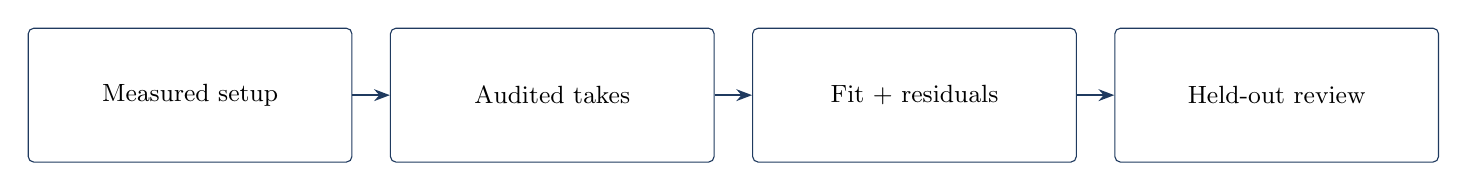
\begin{tikzpicture}\node[box,text width=39mm,minimum height=17mm] (a0) at (0.0,0) {Measured setup};\node[box,text width=39mm,minimum height=17mm] (a1) at (4.6,0) {Audited takes};\draw[flow] (a0.east)--(a1.west);\node[box,text width=39mm,minimum height=17mm] (a2) at (9.2,0) {Fit + residuals};\draw[flow] (a1.east)--(a2.west);\node[box,text width=39mm,minimum height=17mm] (a3) at (13.799999999999999,0) {Held-out review};\draw[flow] (a2.east)--(a3.west);\end{tikzpicture}}{Factory geometry remains operating data; generated candidates are not installed.}
\vfill\takeaway{Why WBR cares: an optimizer cannot repair wrong units, missing frames or a warped target.}
\note{base/main-v4-91p.tex; base/main.tex Phase 8; docs/PROJECT\_STATE.md and NEXT\_GATE.md. Offline teaching synthesis; no new physical evidence.}
\end{frame}
\begin{frame}{Intrinsics and stereo: validate the operating model}
\evidence{MEASURED readback / ASSUMED operating choice}
\deckitems{\item Operating candidate is Rectified, 640$\times$480 Y8, factory equal projections.\item Do not refit physical lens distortion from already rectified pixels blindly.\item S take checks rows, fixed-K reprojection, coverage and depth scale.}
\vfill\takeaway{A fitted PinHole candidate is reviewed separately before deployment.}
\note{docs/D435I\_CALIBRATION\_PLAN.md §1–2 and calibration/lab/README.md. Y8 ASIC rectification is INFERRED in the plan, not independently verified here. No operating YAML is overwritten.}
\end{frame}
\begin{frame}{Measured target: a 6$\times$4 printable AprilGrid}
\evidence{SOURCE-SUPPORTED target / measured dimensions OPEN}
\deckitems{\item Use A3 45 mm tags, spacing ratio 0.3; A4 30 mm is the fallback.\item Laser print at actual size; measure black edges, axis stretch and flatness.\item Replace nominal tagSize in a session copy; keep tagRows = 4.}
\vfill\takeaway{The plan’s stale six-row paragraph loses to the actual 6$\times$4 target files.}
\note{calibration/aprilgrid/README.md and YAMLs. A3 working range 0.4–0.8 m; A4 0.3–0.5 m. Earlier 6$\times$6/80 mm target is superseded.}
\end{frame}
\begin{frame}{Camera–IMU calibration: excite observable motion}
\evidence{KNOWN method}
\deckitems{\item Kalibr uses a fixed measured grid and fixed factory camera chain.\item Record C1–C3 with translation and rotation about all three axes.\item Keep 5–10 s still at each end, emitter off, no impacts, blur or cable pull.}
\vfill\takeaway{An attractive transform can coexist with bad residuals.}
\note{Calibration plan §3; lab allows 60–120 s, default 120 s in plan. Study lab uses 60 s C takes to fit RAM; separate S is 120 s only when reserve permits.}
\end{frame}
\begin{frame}{Kalibr transform: worked inversion}
\evidence{SOURCE-SUPPORTED convention / CALCULATED example}
\deckitems{\item Kalibr T\_cam\_imu maps IMU$\to$camera; ORB T\_b\_c1 maps camera$\to$IMU.\item For R = I, inversion negates t; for general R use −R$^{T}$t.\item ORB b refers to the D435i IMU, never STM32 imu\_body.}
\par\medskip \[T_{b c1}=T_{cam\,imu}^{-1},\quad t_{b c1}\approx[-5.52,\;5.10,\;11.74]^T\;\mathrm{mm}\]
\vfill\takeaway{Run basis-vector and inverse-composition checks before using a candidate.}
\note{The displayed camera$\to$IMU translation is the nominal factory comparison, not a Kalibr result. A hypothetical Kalibr identity-R translation of [5.52,-5.10,-11.74] mm inverts to this nominal vector.}
\end{frame}
\begin{frame}{Kalibr time: worked sign and application boundary}
\evidence{SOURCE-SUPPORTED sign / CALCULATED illustrative}
\deckitems{\item Convention: t\_imu = t\_cam + shift seconds.\item Illustrative +2 ms maps camera time 1.000 s to IMU time 1.002 s.\item Correct both image stamps once before coverage/association; keep raw audit.}
\par\medskip \[t_{cam,corrected}=t_{cam,raw}+0.002\;\mathrm{s}\]
\vfill\takeaway{ORB has no time-offset YAML key; runtime hook availability is OPEN.}
\note{docs/D435I\_CALIBRATION\_PLAN.md §4. Do not move IMU too, do not shift exported inputs twice, do not invent --cam-imu-shift-ms as an available flag.}
\end{frame}
\begin{frame}{Calibration: proposed review thresholds}
\evidence{ASSUMED from current calibration plan}
\begin{tabular}{@{}L{65mm}L{115mm}@{}}\toprule
\textbf{Check} & \textbf{ASSUMED review threshold}\\\midrule
S image geometry & RMS $\leq$0.5 px; row median $\leq$0.3 px, p95 $\leq$1 px.\\[6pt]
S coverage / depth & $\geq$100 pairs, four quadrants; depth error $\leq$2\%.\\[6pt]
C repeated extrinsics & Spread $\leq$3 mm / 1$^\circ$; CAD comparison $\leq$5 mm / 2$^\circ$.\\[6pt]
C time shifts & At least 3 takes; max−min $\leq$1 ms.\\[6pt]\bottomrule\end{tabular}\vfill\takeaway{These are ASSUMED review thresholds, not manufacturer specs or gate PASS.}
\note{Study synthesis from base/main-v4-91p.tex, updated against base/main.tex. No new physical evidence; every gate remains OPEN.}
\end{frame}
\begin{frame}{Calibration: common mistake and check yourself}
\evidence{KNOWN method}
\deckitems{\item Mistake: use an optimizer’s tiny uncertainty as proof of physical accuracy.\item Check residual patterns, detections, data timing and held-out repeatability.\item Question: can online bias estimates fix unknown IMU scale/misalignment?}
\vfill\takeaway{Keep calibration OPEN when the data cannot identify the parameter.}
\note{Answer: no. Online bias can address offsets; it does not establish scale/misalignment. Six static gravity poses diagnose accel, but do not determine gyro scale without known rotation or observable dynamic calibration.}
\end{frame}
\begin{frame}{Calibration: answer}
\evidence{KNOWN method / WBR qualification OPEN}
\deckitems{\item No. Online bias estimates address offsets, not a verified scale or axis-misalignment model.\item Six static gravity poses diagnose accelerometer behavior; gyro scale needs known-rate or observable dynamic evidence.}
\vfill\takeaway{Use this answer to check the reasoning on the preceding page.}
\note{base/main-v4-91p.tex; base/main.tex Phase 8; docs/PROJECT\_STATE.md and NEXT\_GATE.md. Offline teaching synthesis; no new physical evidence.}
\end{frame}
\begin{frame}{ORB-SLAM3: work shared across threads}
\evidence{KNOWN method}
\deckitems{\item SLAM = simultaneous localization and mapping; ORB = Oriented FAST and Rotated BRIEF.\item Tracking handles each stereo input, IMU prediction and pose optimization.\item Local mapping optimizes nearby keyframes and scene points.\item Loop closing corrects revisits; Atlas may hold multiple maps.}
\par\medskip \coursefigure{orb}{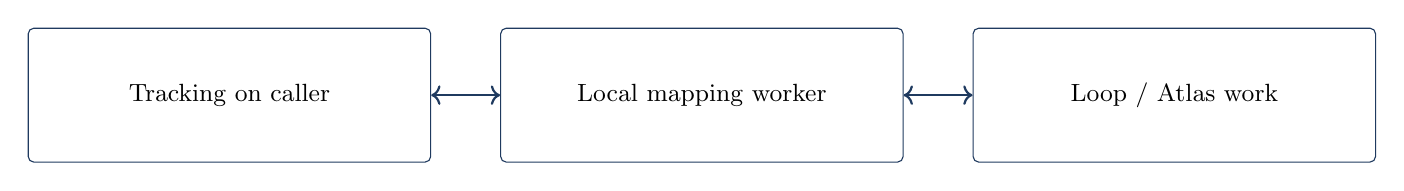
\begin{tikzpicture}\node[box,text width=49mm,minimum height=17mm] (a0) at (0.0,0) {Tracking on caller};\node[box,text width=49mm,minimum height=17mm] (a1) at (6.0,0) {Local mapping worker};\draw[flow,<->] (a0.east)--(a1.west);\node[box,text width=49mm,minimum height=17mm] (a2) at (12.0,0) {Loop / Atlas work};\draw[flow,<->] (a1.east)--(a2.west);\end{tikzpicture}}{Cooperating roles; bidirectional links show shared work.}
\vfill\takeaway{Why WBR cares: a nonempty trajectory may hide resets or a map switch.}
\note{Study synthesis from base/main-v4-91p.tex, updated against base/main.tex. No new physical evidence; every gate remains OPEN.}
\end{frame}
\begin{frame}{Tracking: account for every image interval}
\evidence{KNOWN method}
\deckitems{\item Pair left/right by original identity and valid time relation.\item Supply covered IMU samples; reject duplicate/backward time and gaps.\item Log tracking state, lost frames, resets, map identity and initialization.}
\vfill\takeaway{A viewer or successful launch is not a tracking verdict.}
\note{Study synthesis from base/main-v4-91p.tex, updated against base/main.tex. No new physical evidence; every gate remains OPEN.}
\end{frame}
\begin{frame}{Initialization: stereo scale does not solve everything}
\evidence{KNOWN method}
\deckitems{\item Stereo baseline supplies metric geometry under valid calibration.\item Gravity, velocity and inertial biases still need sufficient excitation.\item A still take can end cleanly with no initialized map.}
\vfill\takeaway{Use smooth multi-axis motion; keep target calibration and VIO routes separate.}
\note{Study synthesis from base/main-v4-91p.tex, updated against base/main.tex. No new physical evidence; every gate remains OPEN.}
\end{frame}
\begin{frame}{Initialization: check yourself}
\evidence{KNOWN method / illustrative question}
\deckitems{\item A 15 s still take exits cleanly with no map. Does this establish successful inertial initialization?}
\vfill\takeaway{Work out your answer before turning the page.}
\note{base/main-v4-91p.tex; base/main.tex Phase 8; docs/PROJECT\_STATE.md and NEXT\_GATE.md. Offline teaching synthesis; no new physical evidence.}
\end{frame}
\begin{frame}{Initialization: answer}
\evidence{KNOWN method / illustrative question}
\deckitems{\item No. A clean exit and an initialized map are different observations.\item Use smooth excitation, valid timing and initialization events. Still data can test acquisition without identifying all inertial state.}
\vfill\takeaway{Explain the evidence that would distinguish the two cases.}
\note{base/main-v4-91p.tex; base/main.tex Phase 8; docs/PROJECT\_STATE.md and NEXT\_GATE.md. Offline teaching synthesis; no new physical evidence.}
\end{frame}
\begin{frame}{Association: worked interpolation}
\evidence{CALCULATED illustrative}
\deckitems{\item Illustrative accel values: 1.0 at 10 ms and 3.0 at 20 ms.\item At gyro time 15 ms, bracketed linear interpolation gives 2.0.\item Outside the bracket or across an invalid gap, reject rather than extrapolate.}
\par\medskip \[a(15)=1+\frac{15-10}{20-10}(3-1)=2\]
\vfill\takeaway{Preserve both raw accel and the derived gyro-grid value.}
\note{Study synthesis from base/main-v4-91p.tex, updated against base/main.tex. No new physical evidence; every gate remains OPEN.}
\end{frame}
\begin{frame}{Mapping and Atlas: distinguish map state from file output}
\evidence{KNOWN method / WBR qualification OPEN}
\deckitems{\item Keyframes retain selected views, poses and constraints; local mapping improves nearby structure.\item Atlas can start another map after loss and later merge maps or accept loop corrections.\item A nonempty trajectory can hide multiple maps, resets or relocalizations.}
\par\medskip \coursefigure{b2-atlas}{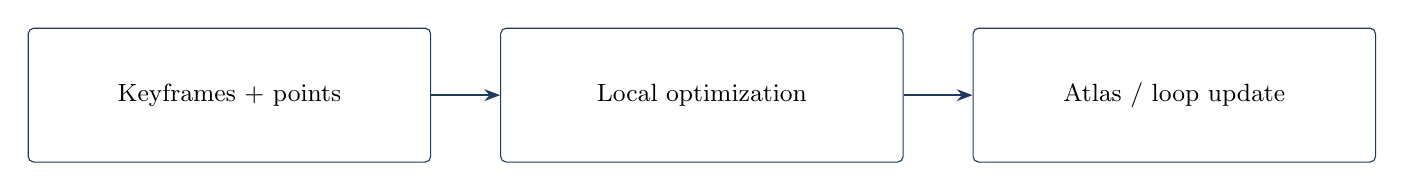
\begin{tikzpicture}\node[box,text width=49mm,minimum height=17mm] (a0) at (0.0,0) {Keyframes + points};\node[box,text width=49mm,minimum height=17mm] (a1) at (6.0,0) {Local optimization};\draw[flow] (a0.east)--(a1.west);\node[box,text width=49mm,minimum height=17mm] (a2) at (12.0,0) {Atlas / loop update};\draw[flow] (a1.east)--(a2.west);\end{tikzpicture}}{Reference changes require state and map IDs; they are not just visual improvements.}
\vfill\takeaway{Why WBR cares: downstream state must be re-established after reference changes.}
\note{base/main-v4-91p.tex; base/main.tex Phase 8; docs/PROJECT\_STATE.md and NEXT\_GATE.md. Offline teaching synthesis; no new physical evidence.}
\end{frame}
\begin{frame}{Atlas: worked reset example}
\evidence{CALCULATED illustrative / actual event instrumentation OPEN}
\deckitems{\item Illustrative run creates map 7, loses tracking, then initializes map 8 at a new origin.\item Both exported segments may contain finite poses; joining their xyz values makes a fictitious path.\item Keep map/session/reset IDs and review the relation before comparing or forwarding segments.}
\vfill\takeaway{Common mistake: a continuous file is assumed to be a continuous coordinate frame.}
\note{base/main-v4-91p.tex; base/main.tex Phase 8; docs/PROJECT\_STATE.md and NEXT\_GATE.md. Offline teaching synthesis; no new physical evidence.}
\end{frame}
\begin{frame}{Atlas state: check yourself}
\evidence{KNOWN method / illustrative question}
\deckitems{\item A trajectory has more rows after relocalization. Does that prove one continuous successful trial?}
\vfill\takeaway{Work out your answer before turning the page.}
\note{base/main-v4-91p.tex; base/main.tex Phase 8; docs/PROJECT\_STATE.md and NEXT\_GATE.md. Offline teaching synthesis; no new physical evidence.}
\end{frame}
\begin{frame}{Atlas state: answer}
\evidence{KNOWN method / illustrative question}
\deckitems{\item No. Row count alone cannot reveal map changes, resets or the duration of lost tracking.\item Retain state events and all attempts, then evaluate each supported frame segment.}
\vfill\takeaway{Explain the evidence that would distinguish the two cases.}
\note{base/main-v4-91p.tex; base/main.tex Phase 8; docs/PROJECT\_STATE.md and NEXT\_GATE.md. Offline teaching synthesis; no new physical evidence.}
\end{frame}
\begin{frame}{Settings audit before feature tuning}
\evidence{SOURCE-SUPPORTED contract / gate OPEN}
\begin{tabular}{@{}L{64mm}L{116mm}@{}}\toprule
\textbf{Parser group} & \textbf{Verify first}\\\midrule
Camera / Stereo & Model, selected rectification, dimensions, focal pixels and positive baseline.\\[6pt]
IMU.T\_b\_c1 & Camera$\to$estimator-IMU direction; metres; matrix layout and basis tests.\\[6pt]
IMU frequency / noise & Input grid and continuous units; no double discretization.\\[6pt]
ORBextractor & Only then inspect feature count, pyramid and FAST thresholds.\\[6pt]\bottomrule\end{tabular}\vfill\takeaway{A settings change must answer a measured failure, using the pinned parser.}
\note{v4 §3.28; calibration plan Settings.cc and Tracking.cc source audit.}
\end{frame}
\begin{frame}{Numeric IMU settings: examples are not measurements}
\evidence{ASSUMED candidate values / SOURCE-SUPPORTED units}
\begin{tabular}{@{}L{65mm}L{115mm}@{}}\toprule
\textbf{Key} & \textbf{ASSUMED example / continuous-time units}\\\midrule
IMU.NoiseGyro & 0.001 rad/s/$\sqrt{\vphantom{x}}$Hz\\[6pt]
IMU.NoiseAcc & 0.01 m/s$^2$/$\sqrt{\vphantom{x}}$Hz\\[6pt]
IMU.GyroWalk & 0.000001 rad/s$^2$/$\sqrt{\vphantom{x}}$Hz\\[6pt]
IMU.AccWalk & 0.0001 m/s$^3$/$\sqrt{\vphantom{x}}$Hz\\[6pt]\bottomrule\end{tabular}\vfill\takeaway{Unit-specific values remain UNKNOWN until supported Allan fitting.}
\note{Current calibration plan register and §5. These example fields originate in the current candidate, not a new-unit noise measurement.}
\end{frame}
\begin{frame}{Numeric IMU contract: scaling happens exactly once}
\evidence{SOURCE-SUPPORTED scaling / CALCULATED example}
\deckitems{\item IMU.Frequency = 200 describes the reviewed combined grid, not the raw 100 Hz accelerometer.\item The pinned tracker multiplies noise density by $\sqrt{\vphantom{x}}$f and divides walk by $\sqrt{\vphantom{x}}$f.\item At 200 Hz, example GyroWalk 1e-6 becomes about 7.07e-8 per step before covariance construction.}
\par\medskip \[\sigma_{n,d}=N\sqrt f,\qquad\sigma_{w,d}=K/\sqrt f\]
\vfill\takeaway{Keep the YAML continuous; interpolation correlation is still a model limitation.}
\note{base/main-v4-91p.tex; base/main.tex Phase 8; docs/PROJECT\_STATE.md and NEXT\_GATE.md. Offline teaching synthesis; no new physical evidence.}
\end{frame}
\begin{frame}{ORB: common mistake and check yourself}
\evidence{KNOWN method}
\deckitems{\item Mistake: increase feature count to hide dropped data or wrong geometry.\item Debug power $\to$ USB $\to$ raw streams $\to$ clocks $\to$ ROS/bag $\to$ calibration $\to$ ORB.\item Question: does offline replay establish live throughput or fresh output?}
\vfill\takeaway{Use immutable inputs to isolate code changes, then test live scheduling.}
\note{Answer: no. Offline playback removes acquisition deadlines; mapping/loop workers still cause scheduling variation. Live age, queueing, drops, power and resource limits need their own evidence.}
\end{frame}
\begin{frame}{ORB: answer}
\evidence{KNOWN method / WBR qualification OPEN}
\deckitems{\item No. Offline replay does not establish live deadlines, throughput or fresh output.\item Acquire loaded live queue/age/drop and platform traces after immutable offline input is validated.}
\vfill\takeaway{Use this answer to check the reasoning on the preceding page.}
\note{base/main-v4-91p.tex; base/main.tex Phase 8; docs/PROJECT\_STATE.md and NEXT\_GATE.md. Offline teaching synthesis; no new physical evidence.}
\end{frame}
\begin{frame}{Gate ladder: prerequisites remain OPEN}
\evidence{SOURCE-SUPPORTED current project state}
\begin{tabular}{@{}L{45mm}L{135mm}@{}}\toprule
\textbf{Gate} & \textbf{Meaning / current evidence}\\\midrule
N0 / N1 & Stable platform / current-unit access; OPEN.\\[6pt]
N2 / N3 & Exact raw soak / ROS record-replay; OPEN, active N3.\\[6pt]
N4A & Known EuRoC dataset on Pi; strong historical evidence, OPEN.\\[6pt]
N4B / N4C & D435i offline / live; no qualified camera trajectory.\\[6pt]\bottomrule\end{tabular}\vfill\takeaway{N4A is a separate branch; it cannot accept the camera prerequisites.}
\note{Study synthesis from base/main-v4-91p.tex, updated against base/main.tex. No new physical evidence; every gate remains OPEN.}
\end{frame}
\begin{frame}{Gate ladder: measurement and controller boundary}
\evidence{OPEN / N5–N7 not started}
\begin{tabular}{@{}L{40mm}L{140mm}@{}}\toprule
\textbf{Gate} & \textbf{Required evidence}\\\midrule
N5 & Reproducible accuracy/continuity/latency/resources.\\[6pt]
N6 & Health semantics: stale, invalid, reset, unknown-age fixtures.\\[6pt]
N7 & Staged controller integration, independent local control.\\[6pt]\bottomrule\end{tabular}\vfill\takeaway{WBR age budgets and physical safety bounds remain UNKNOWN.}
\note{Study synthesis from base/main-v4-91p.tex, updated against base/main.tex. No new physical evidence; every gate remains OPEN.}
\end{frame}
\begin{frame}{Gate dependencies: branch on the experiment input}
\evidence{KNOWN method / WBR qualification OPEN}
\deckitems{\item N0 supports the independent EuRoC N4A baseline; that dataset does not test D435i acquisition.\item Camera N4B requires N1–N3 plus stereo extension and calibration; N4C adds live scheduling.\item N5 measurement, N6 semantics and N7 controlled integration need separate evidence.}
\par\medskip \coursefigure{b2-gates}{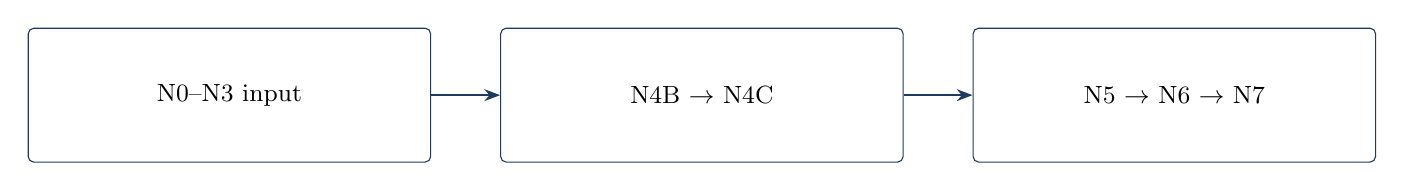
\begin{tikzpicture}\node[box,text width=49mm,minimum height=17mm] (a0) at (0.0,0) {N0–N3 input};\node[box,text width=49mm,minimum height=17mm] (a1) at (6.0,0) {N4B $\to$ N4C};\draw[flow] (a0.east)--(a1.west);\node[box,text width=49mm,minimum height=17mm] (a2) at (12.0,0) {N5 $\to$ N6 $\to$ N7};\draw[flow] (a1.east)--(a2.west);\end{tikzpicture}}{N4A is a separate N0$\to$EuRoC branch; every current gate remains OPEN.}
\vfill\takeaway{Why WBR cares: identify the claim before deciding which prerequisites apply.}
\note{base/main-v4-91p.tex; base/main.tex Phase 8; docs/PROJECT\_STATE.md and NEXT\_GATE.md. Offline teaching synthesis; no new physical evidence.}
\end{frame}
\begin{frame}{N0 acceptance and diagnosis}
\evidence{SOURCE-SUPPORTED contract / gate OPEN}
\begin{tabular}{@{}L{95mm}L{85mm}@{}}\toprule
\textbf{Required evidence} & \textbf{If it fails}\\\midrule
ARM64, Ubuntu 24.04, ROS 2 Jazzy & Reconcile actual OS/package inventory before sensor work.\\[6pt]
UTC synchronized; power flags 0x0 & Inspect time service or supply/cable; retain sticky faults.\\[6pt]
Temperature <75$^\circ$C; available RAM $\geq$512 MiB & Inspect cooling and competing memory load.\\[6pt]\bottomrule\end{tabular}\vfill\takeaway{Idle readiness must be rechecked under capture and estimator load.}
\note{v4 §4.2 acceptance table; archived PHASE\_A\_RUNBOOK. Values are existing project requirements, not newly measured results.}
\end{frame}
\begin{frame}{N1 acceptance and diagnosis}
\evidence{SOURCE-SUPPORTED contract / gate OPEN}
\begin{tabular}{@{}L{95mm}L{85mm}@{}}\toprule
\textbf{Required evidence} & \textbf{If it fails}\\\midrule
Camera own direct branch $\geq$5000M & At 480M inspect cable, port and hubs before streaming.\\[6pt]
Video and HID/IIO access; no competing owner & Inspect exact device permissions and process ownership.\\[6pt]
Sealed identity/host/boot receipt $\leq$2 h old & Renew after reboot/topology change; separate serial fields.\\[6pt]\bottomrule\end{tabular}\vfill\takeaway{A root hub at 5000M does not qualify its camera child.}
\note{v4 §4.3; N1 source and archived runbook. No broad permission changes prescribed.}
\end{frame}
\begin{frame}{N2 content, health and actual acceptance}
\evidence{SOURCE-SUPPORTED contract / gate OPEN}
\begin{tabular}{@{}L{98mm}L{82mm}@{}}\toprule
\textbf{Required evidence} & \textbf{If it fails}\\\midrule
20 / 105 / mandatory 300 s, clean shutdown & Keep the failed stage and stop downstream acceptance.\\[6pt]
Coherent Y8 images; finite plausible motion & Inspect pixels, dimensions, units and exact stream profile.\\[6pt]
Clean kernel/SDK and 1 Hz platform health & Return to power/USB before blaming an estimator.\\[6pt]
Human review; warning and startup offsets retained & Leave OPEN until the actual review is complete.\\[6pt]\bottomrule\end{tabular}\vfill\takeaway{N2 rate bands on the next page are necessary but not sufficient.}
\note{v4 §4.4–4.5, source tables preserved semantically; exact staged commands remain in S1.3/R.}
\end{frame}
\begin{frame}{N3 acceptance and diagnosis}
\evidence{SOURCE-SUPPORTED contract / gate OPEN}
\begin{tabular}{@{}L{92mm}L{88mm}@{}}\toprule
\textbf{Required evidence} & \textbf{If it fails}\\\midrule
60 s live plus delivery under recorder load & Power/raw first, then graph/QoS and durable storage.\\[6pt]
Exact ten-topic baseline; parameters/types/TF & Inspect actual graph and durable context, not launch intent.\\[6pt]
Final bag and exact complete replay & Reconcile count, order, header and decoded payload hashes.\\[6pt]
No live contamination; clean player/observer stop & Stop the camera and isolate replay in domain 43.\\[6pt]\bottomrule\end{tabular}\vfill\takeaway{The strict baseline is IR1/15; stereo/30 needs separate evidence.}
\note{v4 §4.6–4.7 acceptance; n3\_record.py and n3\_bag.py. Static audit cannot establish camera behavior.}
\end{frame}
\begin{frame}{N3 content checks beyond delivery rates}
\evidence{SOURCE-SUPPORTED runbook proposals / no gate PASS}
\begin{tabular}{@{}L{96mm}L{84mm}@{}}\toprule
\textbf{Runbook proposal} & \textbf{Interpretation / failure branch}\\\midrule
Stationary mean gyro norm $\leq$0.10 rad/s & Use finite raw vectors and a declared stationary interval.\\[6pt]
Stationary mean accel norm 9.0–10.5 m/s$^2$ & Check raw units and frame before claiming plausible gravity.\\[6pt]
Zero incomplete/corrupt notifications & Inspect the unfiltered startup-to-stop SDK/kernel logs.\\[6pt]\bottomrule\end{tabular}\vfill\takeaway{These engineering proposals do not establish calibrated camera–IMU timing.}
\note{v4 §4.7 content table; docs/RPI5\_NATIVE\_PERCEPTION\_BRINGUP.md cited there. Do not confuse 0.10 rad/s bring-up screening with the stricter ASSUMED 0.01 rad/s calibration diagnostic.}
\end{frame}
\begin{frame}{Storage receipts: old baseline and newer exception}
\evidence{SOURCE-SUPPORTED old contract / ASSUMED newer margin / OPEN}
\begin{tabular}{@{}L{65mm}L{115mm}@{}}\toprule
\textbf{Policy} & \textbf{Requirement / unresolved boundary}\\\midrule
Archived strict N3 & External UUID; $\geq$1 GiB and $\geq$60 s; overall and worst 64 MiB batch $\geq$9.216 MB/s.\\[6pt]
Archived readback & Matching SHA-256, cleanup and 10 GiB retained headroom.\\[6pt]
Approved 128 GB-card exception & Take-length/larger-file test $\geq$27.6 MB/s; $\geq$2$\times$ take plus OS reserve.\\[6pt]\bottomrule\end{tabular}\vfill\takeaway{The old runner needs reviewed card-receipt compatibility; never manufacture acceptance.}
\note{v4 storage table; current calibration plan card decision. Old margin was for IR1, not qualification of stereo/30.}
\end{frame}
\begin{frame}{Stereo extension: preserve the accepted baseline}
\evidence{KNOWN method / WBR qualification OPEN}
\deckitems{\item N2/N3 qualify IR1 at 15 Hz with raw motion; keep those records unchanged.\item The stereo extension adds IR2, 30 Hz paired load, both projections and pairing evidence.\item It must recheck bandwidth, storage, stamps and geometry rather than inherit an IR1 verdict.}
\par\medskip \coursefigure{b2-extension}{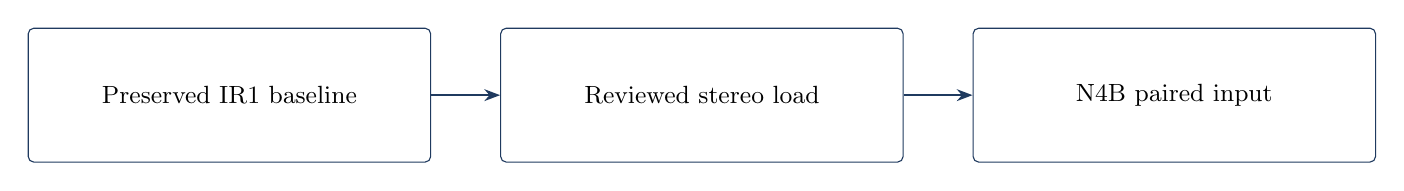
\begin{tikzpicture}\node[box,text width=49mm,minimum height=17mm] (a0) at (0.0,0) {Preserved IR1 baseline};\node[box,text width=49mm,minimum height=17mm] (a1) at (6.0,0) {Reviewed stereo load};\draw[flow] (a0.east)--(a1.west);\node[box,text width=49mm,minimum height=17mm] (a2) at (12.0,0) {N4B paired input};\draw[flow] (a1.east)--(a2.west);\end{tikzpicture}}{One branch extends the input contract; it does not rewrite old evidence.}
\vfill\takeaway{A mono-inertial adapter or an IR2 topic name does not establish stereo readiness.}
\note{base/main-v4-91p.tex; base/main.tex Phase 8; docs/PROJECT\_STATE.md and NEXT\_GATE.md. Offline teaching synthesis; no new physical evidence.}
\end{frame}
\begin{frame}{N4A: known-dataset acceptance and diagnosis}
\evidence{SOURCE-SUPPORTED contract / gate OPEN}
\begin{tabular}{@{}L{91mm}L{89mm}@{}}\toprule
\textbf{Contract} & \textbf{Evidence / failure branch}\\\midrule
N0; pinned binary, libraries, settings and MH01 & Build/link error $\to$ dependencies; empty images $\to$ reader paths.\\[6pt]
Finite ordered exports and supported coverage & Audit dataset epochs, origin, quaternion and input hashes.\\[6pt]
Repeated initialization / all attempts & No inertial init $\to$ settings, timing and motion.\\[6pt]
ATE/RPE and continuity budgets UNKNOWN & Measured ATE supports the build; power and review keep gate OPEN.\\[6pt]\bottomrule\end{tabular}\vfill\takeaway{N4A never qualifies camera transport or unit calibration.}
\note{v4 §4.9; Phase-8 excludes numeric historical RPE/paper comparator, while retaining ATE.}
\end{frame}
\begin{frame}{N4B: offline D435i acceptance and diagnosis}
\evidence{SOURCE-SUPPORTED contract / gate OPEN}
\begin{tabular}{@{}L{92mm}L{88mm}@{}}\toprule
\textbf{Contract} & \textbf{Evidence / failure branch}\\\midrule
N3 + stereo extension + calibrated inputs & Direct SDK diagnostics cannot bypass formal prerequisites.\\[6pt]
Lossless pairs, valid time and IMU coverage & Vertical mismatch $\to$ geometry; missing brackets $\to$ raw motion.\\[6pt]
Geometry, noise and time offset supported & Review residuals/held-out repeats before feature tuning.\\[6pt]
Repeatable finite state; budgets UNKNOWN & Retain crashes and resets; absent reference means accuracy UNKNOWN.\\[6pt]\bottomrule\end{tabular}\vfill\takeaway{A build, short recording or still replay is not a qualified motion trajectory.}
\note{base/main-v4-91p.tex; base/main.tex Phase 8; docs/PROJECT\_STATE.md and NEXT\_GATE.md. Offline teaching synthesis; no new physical evidence.}
\end{frame}
\begin{frame}{N4B provenance: connect raw data to each pose}
\evidence{KNOWN method / WBR qualification OPEN}
\deckitems{\item The native recorder creates stereo\_imu.db3 and timestamps.csv; ordinary ROS bags use a different schema.\item The conversion manifest links raw hash, converter version, pixels, exact ns and settings.\item Retain rejected samples and interpolation decisions; do not sort or invent missing motion.}
\par\medskip \coursefigure{b2-provenance}{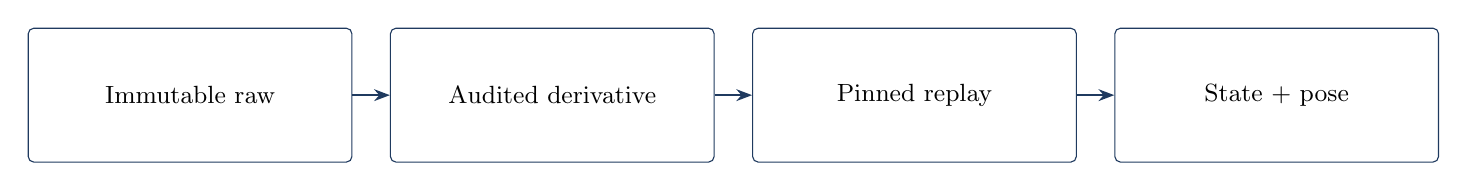
\begin{tikzpicture}\node[box,text width=39mm,minimum height=17mm] (a0) at (0.0,0) {Immutable raw};\node[box,text width=39mm,minimum height=17mm] (a1) at (4.6,0) {Audited derivative};\draw[flow] (a0.east)--(a1.west);\node[box,text width=39mm,minimum height=17mm] (a2) at (9.2,0) {Pinned replay};\draw[flow] (a1.east)--(a2.west);\node[box,text width=39mm,minimum height=17mm] (a3) at (13.799999999999999,0) {State + pose};\draw[flow] (a2.east)--(a3.west);\end{tikzpicture}}{Native and ROS paths need separately validated adapters.}
\vfill\takeaway{Why WBR cares: replay comparisons are useful only when the input has stayed fixed.}
\note{base/main-v4-91p.tex; base/main.tex Phase 8; docs/PROJECT\_STATE.md and NEXT\_GATE.md. Offline teaching synthesis; no new physical evidence.}
\end{frame}
\begin{frame}{N4C: live acceptance and diagnosis}
\evidence{SOURCE-SUPPORTED contract / gate OPEN}
\begin{tabular}{@{}L{91mm}L{89mm}@{}}\toprule
\textbf{Contract} & \textbf{Evidence / failure branch}\\\midrule
Accepted N4B; renewed stereo acquisition & Same geometry/settings, fresh physical receipts under load.\\[6pt]
Initialization and continuity budgets UNKNOWN & Retain eligible attempts, lost intervals and resets.\\[6pt]
Latency and queue bounds UNKNOWN & Same-clock events; mapped capture age includes uncertainty.\\[6pt]
Offline works, live lags & Inspect wrapper/DDS/executor/queues, then loaded power/thermal.\\[6pt]\bottomrule\end{tabular}\vfill\takeaway{Live camera mode remains unattempted in the controlling Phase-8 evidence.}
\note{base/main-v4-91p.tex; base/main.tex Phase 8; docs/PROJECT\_STATE.md and NEXT\_GATE.md. Offline teaching synthesis; no new physical evidence.}
\end{frame}
\begin{frame}{N5: measurement acceptance and diagnosis}
\evidence{SOURCE-SUPPORTED contract / gate OPEN}
\begin{tabular}{@{}L{87mm}L{93mm}@{}}\toprule
\textbf{Contract} & \textbf{Evidence / failure branch}\\\midrule
Valid reference for ATE/RPE & Audit frames, association, overlap and rigid alignment.\\[6pt]
P50/P95/P99, init/loss, sample counts & Name event interval and clock; averages hide tail stalls.\\[6pt]
CPU/thermal/RAM, losses and queue series & Join events; unavailable counters remain UNKNOWN.\\[6pt]
Frozen hypotheses and all attempts & At least three offline repeats is a planned minimum.\\[6pt]\bottomrule\end{tabular}\vfill\takeaway{Numeric performance budgets remain UNKNOWN; a report is not automatic acceptance.}
\note{v4 §4.12 and §5.6–5.10; no new N5 executable or numeric acceptance budget exists.}
\end{frame}
\begin{frame}{N6: health acceptance and diagnosis}
\evidence{SOURCE-SUPPORTED contract / gate OPEN}
\begin{tabular}{@{}L{91mm}L{89mm}@{}}\toprule
\textbf{Contract} & \textbf{Evidence / failure branch}\\\midrule
Reject every declared invalid fixture & Expected/actual state and reason, on synthetic event time.\\[6pt]
Source-age bound $\leq$Amax; Amax UNKNOWN & Clock relation, wrap and delay fixtures; receipt alone is insufficient.\\[6pt]
Explicit reset/session/frame re-establishment & Old session accepted $\to$ protocol; wrap failure $\to$ receiver clock.\\[6pt]\bottomrule\end{tabular}\vfill\takeaway{A reviewed receiver harness is planned; the CN demo is not WBR N6 acceptance.}
\note{v4 §4.13; canonical architecture. Distinct from source-defined OS v3 provisional timeouts.}
\end{frame}
\begin{frame}{N7: boundary acceptance and diagnosis}
\evidence{SOURCE-SUPPORTED contract / gate OPEN}
\begin{tabular}{@{}L{92mm}L{88mm}@{}}\toprule
\textbf{Contract} & \textbf{Evidence / failure branch}\\\midrule
Perception has no safety authority & Ownership/code review plus controlled fault trace.\\[6pt]
Local control retained when Pi is lost & STM32 loop/watchdog/motor-state trace on MCU clock.\\[6pt]
Fallback inside approved budget; bound UNKNOWN & Measured fault-to-local-action interval and safety review.\\[6pt]\bottomrule\end{tabular}\vfill\takeaway{Receiver bench $\to$ approved controlled integration $\to$ separately approved physical test.}
\note{v4 §4.14. No motor-test command or physical balancing claim is supplied.}
\end{frame}
\begin{frame}{N2 thresholds stay exactly as specified}
\evidence{SOURCE-SUPPORTED gate criteria}
\begin{tabular}{@{}L{73mm}L{107mm}@{}}\toprule
\textbf{Stream / condition} & \textbf{Requirement}\\\midrule
IR1 / gyro / accel & 14.25–15.75 / 190–210 / 95–105 Hz.\\[6pt]
Image / motion max gap & $\leq$0.20 s / $\leq$0.05 s.\\[6pt]
Order and image identity & Positive time/frame steps; no missing image frames.\\[6pt]
Durations and health & 20 $\to$ 105 $\to$ 300 s; clean power/kernel; actual review.\\[6pt]\bottomrule\end{tabular}\vfill\takeaway{A 20 s stereo diagnostic is not the 20 s N2 stage.}
\note{Study synthesis from base/main-v4-91p.tex, updated against base/main.tex. No new physical evidence; every gate remains OPEN.}
\end{frame}
\begin{frame}{Dated evidence: what the sources actually establish}
\evidence{MEASURED source-reported diagnostics / all gates OPEN}
\deckitems{\item Phase 8: card gaps, short RAM success, first-frame crash, interrupted repair.\item Later lab source reports rebuild + 15 s still EuRoC-route replay exit 0.\item That still replay has no map; hand-motion tracking and live remain unverified.}
\vfill\takeaway{Keep the later report separate from the Phase-8 historical snapshot.}
\note{base/main.tex Phase 8 controls conflicts with 91p. sources/LAB\_DAY\_2026-10-15-4b63.md opening box is later evidence from 14 Oct night, not independently rerun. CN 16 Oct supply availability is owner-reported, not WBR loaded qualification.}
\end{frame}
\begin{frame}{Gate example, common mistake and check yourself}
\evidence{KNOWN method}
\deckitems{\item Worked case: 15 Hz interior rate with a long start delay misses window coverage.\item Compare N/T and (N−1)/(last−first), plus start/tail silence.\item Question: may a historical gate receipt survive a camera swap or reboot?}
\vfill\takeaway{No tuning can repair evidence from the wrong device or boot.}
\note{Answer: no. N1 receipts are identity/host/boot bound, expire after two hours and need renewal after reboot/topology change. Old-unit N2/N3 does not transfer; keep whole-window and interior statistics.}
\end{frame}
\begin{frame}{Gate receipts: answer}
\evidence{KNOWN method / WBR qualification OPEN}
\deckitems{\item No. A camera swap invalidates unit evidence; reboot or topology change requires a fresh N1.\item N1 is identity/host/boot bound and $\leq$2 h old. The full-request rate and boundaries still need inspection.}
\vfill\takeaway{Use this answer to check the reasoning on the preceding page.}
\note{base/main-v4-91p.tex; base/main.tex Phase 8; docs/PROJECT\_STATE.md and NEXT\_GATE.md. Offline teaching synthesis; no new physical evidence.}
\end{frame}
\begin{frame}{Worked window check: nominal interior, missing coverage}
\evidence{CALCULATED illustrative / SOURCE-SUPPORTED N2 limit}
\deckitems{\item Illustrative request lasts 20 s, but 150 images arrive only from t=10 to t=19.933 s.\item Interior rate is about 15 Hz. Whole-window rate is 150/20 = 7.5 Hz.\item Initial silence is 10 s, far beyond the N2 image-gap requirement of 0.20 s.}
\par\medskip \[r_{whole}=N/T,\quad r_{interior}=(N-1)/(a_N-a_1),\quad B=\max(a_1,T-a_N)\]
\vfill\takeaway{A nominal burst rate cannot accept the requested acquisition window.}
\note{base/main-v4-91p.tex; base/main.tex Phase 8; docs/PROJECT\_STATE.md and NEXT\_GATE.md. Offline teaching synthesis; no new physical evidence.}
\end{frame}
\begin{frame}{Evaluation: the measured EuRoC MH01 baseline}
\evidence{MEASURED historical / N4A OPEN}
\deckitems{\item Historical 4 GB Pi completed three runs with IMU initialization, one map, no resets.\item Absolute Trajectory Error (ATE), rigid-aligned: 0.0415 / 0.0368 / 0.0416 m.\item These are root mean square errors (RMSE); mean RMSE is about 0.040 m.\item Alignment fits rotation and translation only; scale is not fitted.}
\vfill\takeaway{Why WBR cares: known input tests the build without camera adaptation.}
\note{base/main.tex Phase-8 baseline; experiments/2026-10-13-n4a-euroc-mh01/REPORT.md. Under-voltage invalidates a performance verdict; no D435i accuracy claim. Phase-8 excludes later numeric RPE and paper comparator.}
\end{frame}
\begin{frame}{ATE: worked RMS after a declared alignment}
\evidence{CALCULATED illustrative}
\deckitems{\item Illustrative position residuals after SE(3) alignment are 0.03 and 0.04 m.\item RMSE is sqrt((0.03$^2$ + 0.04$^2$)/2) = 0.03536 m.\item Report association tolerance, overlap, excluded frames and failed trials.}
\par\medskip \[\operatorname{ATE}_{RMSE}=\sqrt{\tfrac1n\sum_i\|p_i^{ref}-(Rp_i^{est}+t)\|^2}\]
\vfill\takeaway{An alignment removes gauge freedom; it does not prove frame compatibility.}
\note{Study synthesis from base/main-v4-91p.tex, updated against base/main.tex. No new physical evidence; every gate remains OPEN.}
\end{frame}
\begin{frame}{RPE: relative pose error over a fixed interval}
\evidence{CALCULATED illustrative / historical RPE UNVERIFIED}
\deckitems{\item Illustrative reference relative translation is 1.00 m; estimate is 1.02 m.\item With equal rotation/direction, translation RPE is 0.02 m for that pair.\item Declare delta seconds/metres/frames, endpoint policy and eligible pair count.}
\par\medskip \[E_{ij}=(T_i^{-1}T_j)_{ref}^{-1}(T_i^{-1}T_j)_{est}\]
\vfill\takeaway{Numeric historical RPE remains UNVERIFIED under Phase-8 source restrictions.}
\note{This teaches the metric without reinstating the excluded Phase-7 numeric claims. tools/trajectory\_eval uses first eligible endpoint, no interpolation, overlapping pairs allowed.}
\end{frame}
\begin{frame}{Without ground truth: useful proxies have limits}
\evidence{ASSUMED review protocol / accuracy UNKNOWN}
\deckitems{\item Record initialization time, resets/maps, loss fraction and longest lost interval.\item Use a measured straight segment and return-to-start route with placement uncertainty.\item Loop closure can conceal drift: report pre-loop and final closure separately.}
\vfill\takeaway{Tape scale and closure are proxies, never D435i ATE.}
\note{Calibration plan V1–V3: initialization $\leq$30 s, zero resets, one map, loss $\leq$1\%, none >1 s, route closure/segment error $\leq$2\%, cross-take closure spread $\leq$1 percentage point; all are ASSUMED.}
\end{frame}
\begin{frame}{Evaluation: common mistake and check yourself}
\evidence{KNOWN method}
\deckitems{\item Mistake: fit Sim(3) scale and call the metric-scale stereo result accurate.\item A plausible path or low aligned residual can hide scale, frame and timing errors.\item Question: can 184 s dataset time / 282 s wall time give per-frame P99?}
\vfill\takeaway{Report metric boundaries and evidence eligibility before comparing numbers.}
\note{Answer: no. Startup, vocabulary loading, tracking and shutdown are mixed in wall time. Historical walls 301/282/284 s, peak RSS 823/828/828 MiB and 87/178 live power-fault samples are summaries, not per-frame latency distributions.}
\end{frame}
\begin{frame}{Evaluation: answer}
\evidence{KNOWN method / WBR qualification OPEN}
\deckitems{\item No. Dataset time divided by wall duration cannot recover per-frame P99 latency.\item Wall duration mixes vocabulary loading, tracking and shutdown; keep raw event boundaries on a named clock.}
\vfill\takeaway{Use this answer to check the reasoning on the preceding page.}
\note{base/main-v4-91p.tex; base/main.tex Phase 8; docs/PROJECT\_STATE.md and NEXT\_GATE.md. Offline teaching synthesis; no new physical evidence.}
\end{frame}
\begin{frame}{Trajectory conversion: audit one row first}
\evidence{KNOWN method / WBR qualification OPEN}
\deckitems{\item TUM rows contain seconds, xyz in metres, then quaternion qx qy qz qw.\item EuRoC reference uses ns and qw-first fields. The ORB output format depends on the selected example.\item Check pose direction and physical origin before converting; invert a world-to-camera pose when required.}
\par\medskip \coursefigure{b2-traj}{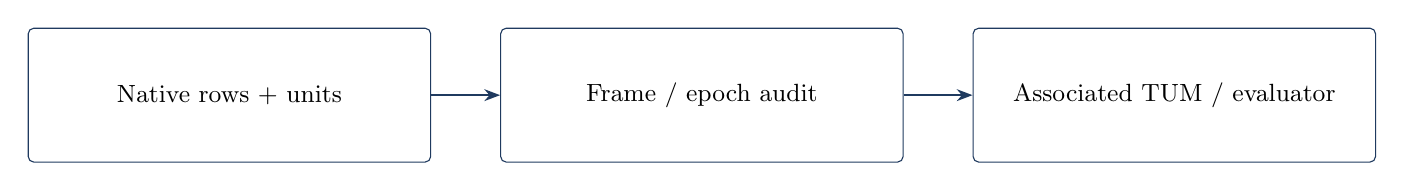
\begin{tikzpicture}\node[box,text width=49mm,minimum height=17mm] (a0) at (0.0,0) {Native rows + units};\node[box,text width=49mm,minimum height=17mm] (a1) at (6.0,0) {Frame / epoch audit};\draw[flow] (a0.east)--(a1.west);\node[box,text width=49mm,minimum height=17mm] (a2) at (12.0,0) {Associated TUM / evaluator};\draw[flow] (a1.east)--(a2.west);\end{tikzpicture}}{Preserve originals and save converter version, argv and rejected rows.}
\vfill\takeaway{Why WBR cares: a converter can create a smooth but physically wrong trajectory.}
\note{v4 §5.4; tools/trajectory\_eval README and selected example output behavior. No universal ORB output origin assumed.}
\end{frame}
\begin{frame}{Trajectory conversion: worked units and quaternion}
\evidence{CALCULATED illustrative / format contract}
\deckitems{\item Illustrative input epoch 1,000,000,000 ns becomes 1.000000000 s.\item Identity quaternion qw,qx,qy,qz = 1,0,0,0 becomes TUM qx,qy,qz,qw = 0,0,0,1.\item Mistake: leave ns in a seconds field or reorder quaternion values without changing their meaning.}
\vfill\takeaway{Save an auditable sample row and confirm rotation normalization.}
\note{base/main-v4-91p.tex; base/main.tex Phase 8; docs/PROJECT\_STATE.md and NEXT\_GATE.md. Offline teaching synthesis; no new physical evidence.}
\end{frame}
\begin{frame}{evo: define the metric before invoking it}
\evidence{SOURCE-SUPPORTED source example / execution OPEN}
\deckitems{\item The source example uses evo\_ape with rigid --align for metric stereo trajectories.\item Its evo\_rpe example selects angle\_deg and a 1 m interval; this is an example, not an acceptance limit.\item Check installed help/version and declare tolerance, pair policy, reference coverage and saved outputs.}
\vfill\takeaway{H7 supplies the audited first-party evaluator; its RPE pairing is not automatically evo-equivalent.}
\note{v4 §5.4 exact example: evo\_ape tum REFERENCE.tum ESTIMATE.tum --align; evo\_rpe tum REFERENCE.tum ESTIMATE.tum --pose\_relation angle\_deg --delta 1 --delta\_unit m. No new copyable command block or runtime execution.}
\end{frame}
\begin{frame}{Percentiles: describe the tail as well as the middle}
\evidence{KNOWN method / WBR qualification OPEN}
\deckitems{\item P50 is the median, P95 covers 95\% and P99 covers 99\% under the declared estimator.\item Name the interval: queue wait, compute, receipt-to-output or supported capture age.\item State sample count, warm-up exclusions, failed runs and the percentile method.}
\par\medskip \coursefigure{b2-percentile}{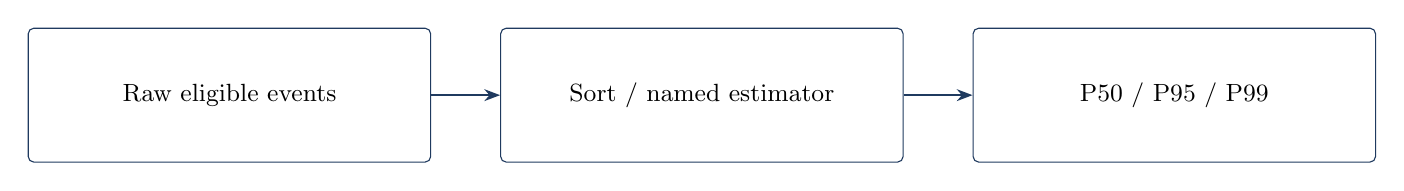
\begin{tikzpicture}\node[box,text width=49mm,minimum height=17mm] (a0) at (0.0,0) {Raw eligible events};\node[box,text width=49mm,minimum height=17mm] (a1) at (6.0,0) {Sort / named estimator};\draw[flow] (a0.east)--(a1.west);\node[box,text width=49mm,minimum height=17mm] (a2) at (12.0,0) {P50 / P95 / P99};\draw[flow] (a1.east)--(a2.west);\end{tikzpicture}}{Do not turn dataset-duration divided by wall-time into a latency percentile.}
\vfill\takeaway{Why WBR cares: occasional old output can matter even when median compute is fast.}
\note{base/main-v4-91p.tex; base/main.tex Phase 8; docs/PROJECT\_STATE.md and NEXT\_GATE.md. Offline teaching synthesis; no new physical evidence.}
\end{frame}
\begin{frame}{Percentiles: worked nearest-rank example}
\evidence{CALCULATED illustrative / nearest-rank estimator}
\deckitems{\item For 100 ordered eligible latencies, nearest-rank P95 is sample 95 and P99 is sample 99.\item If samples 1–94 are 10 ms and 95–100 are 200 ms, P50=10 ms but P95=P99=200 ms.\item With very few samples, a tail percentile has weak support; retain the full event series.}
\par\medskip \[\operatorname{rank}(P_p)=\lceil(p/100)N\rceil\]
\vfill\takeaway{Common mistake: report the mean and hide the six slow events.}
\note{base/main-v4-91p.tex; base/main.tex Phase 8; docs/PROJECT\_STATE.md and NEXT\_GATE.md. Offline teaching synthesis; no new physical evidence.}
\end{frame}
\begin{frame}{Loss and continuity: declare the denominator}
\evidence{CALCULATED illustrative / actual continuity OPEN}
\deckitems{\item Reconcile generated, received, recorded and processed IDs at each boundary.\item Illustrative 3 missing out of 300 expected inputs is 1\% loss; 297/10 s is not a zero-loss proof.\item Count every initialization attempt and lost interval; keep resets, map IDs and trajectory coverage.}
\vfill\takeaway{An absent drop counter remains UNKNOWN even when observed output is regular.}
\note{base/main-v4-91p.tex; base/main.tex Phase 8; docs/PROJECT\_STATE.md and NEXT\_GATE.md. Offline teaching synthesis; no new physical evidence.}
\end{frame}
\begin{frame}{N5 resource series: join causes to events}
\evidence{SOURCE-SUPPORTED contract / gate OPEN}
\begin{tabular}{@{}L{88mm}L{92mm}@{}}\toprule
\textbf{Series} & \textbf{Interpretation}\\\midrule
CPU utilization + clock frequency & State the core normalization; clock throttling changes capacity.\\[6pt]
SoC temperature + raw throttling flags & Join warm-up and faults to queue/compute stalls.\\[6pt]
RSS + MemAvailable + free data space & Separate process footprint, system pressure and disk headroom.\\[6pt]
Queue depth + discard/loss events & Keep clock, units and missing-counter labels explicit.\\[6pt]\bottomrule\end{tabular}\vfill\takeaway{One-Hz health helps context; it can miss a short event and is not an IMU-temperature sensor.}
\note{base/main-v4-91p.tex; base/main.tex Phase 8; docs/PROJECT\_STATE.md and NEXT\_GATE.md. Offline teaching synthesis; no new physical evidence.}
\end{frame}
\begin{frame}{Historical N4A timing and resource evidence}
\evidence{MEASURED historical / performance qualification OPEN}
\begin{tabular}{@{}L{99mm}L{81mm}@{}}\toprule
\textbf{Observed summary} & \textbf{Practical limit}\\\midrule
301 / 282 / 284 s wall for 184 s dataset & Includes load/start/stop; no per-frame percentile.\\[6pt]
Peak RSS 823 / 828 / 828 MiB & A peak is not a memory-pressure time series.\\[6pt]
87 / 178 live power-fault samples; max 63$^\circ$C & Power faults invalidate a processor-speed verdict.\\[6pt]\bottomrule\end{tabular}\vfill\takeaway{Preserve measured summaries while leaving unmeasured timing and joined series UNKNOWN.}
\note{v4 §5.9–5.10 and Phase-8 backups; five-second N4A power samples, not a newly collected time series.}
\end{frame}
\begin{frame}{Measurement design: check yourself}
\evidence{CALCULATED illustrative}
\deckitems{\item Worked case: 20 ms compute follows 300 ms queue wait. May you report 20 ms as end-to-end latency?}
\vfill\takeaway{Work out your answer before turning the page.}
\note{base/main-v4-91p.tex; base/main.tex Phase 8; docs/PROJECT\_STATE.md and NEXT\_GATE.md. Offline teaching synthesis; no new physical evidence.}
\end{frame}
\begin{frame}{Measurement design: answer}
\evidence{CALCULATED illustrative}
\deckitems{\item No. Receipt-to-output is at least 320 ms before emission overhead; physical capture age needs a clock mapping.\item The mistake is to choose the fastest boundary after looking at the result.}
\vfill\takeaway{Explain the evidence that would distinguish the two cases.}
\note{base/main-v4-91p.tex; base/main.tex Phase 8; docs/PROJECT\_STATE.md and NEXT\_GATE.md. Offline teaching synthesis; no new physical evidence.}
\end{frame}
\begin{frame}{Pi$\leftrightarrow$STM32 link: integrity before semantics}
\evidence{KNOWN method}
\deckitems{\item Step 9b bench firmware checks RTT, CRC, sequence, session and silence.\item It runs on F446RE as a link stand-in; NO\_LINK is not OS HOLD or FAILSAFE.\item Why WBR cares: packet integrity and fallback policy are distinct tests.}
\vfill\takeaway{Never flash link-bench firmware and expect the CN/OS supervisor.}
\note{sources/STM32\_LINK\_STEP\_2026-10-15.md; tools/link\_bench/README.md; OS protocol/PROTOCOL.md and newer OS-wt-cn docs/CN\_INTEGRATION.md.}
\end{frame}
\begin{frame}{Planned WBR health envelope}
\evidence{SOURCE-SUPPORTED design intent / WBR interface OPEN}
\begin{tabular}{@{}L{91mm}L{89mm}@{}}\toprule
\textbf{Field family} & \textbf{Receiver purpose}\\\midrule
Version, session and sequence & Reject incompatible data, duplicates and old boots.\\[6pt]
Source epoch/domain and age bound & Separate new transport activity from a fresh estimate.\\[6pt]
Frames, map/reset ID and tracking state & Reject a wrong reference or a map-origin change.\\[6pt]
Pose/velocity and supported uncertainty & Use finite, meaningful fields; covariance support is UNKNOWN.\\[6pt]\bottomrule\end{tabular}\vfill\takeaway{WBR message, rate, transport and age threshold remain unselected.}
\note{v4 §3.30; canonical architecture and decisions. This is not the existing CN wire schema.}
\end{frame}
\begin{frame}{WBR health supervision: semantics before firmware}
\evidence{KNOWN method / WBR qualification OPEN}
\deckitems{\item ABSENT and INITIALIZING supply no usable estimate; FRESH requires every eligibility check.\item Old age becomes STALE; bad fields, frame or reset become INVALID and withdraw optional input.\item A new session or map requires explicit re-establishment, not silent acceptance of its first packet.}
\par\medskip \coursefigure{b2-health}{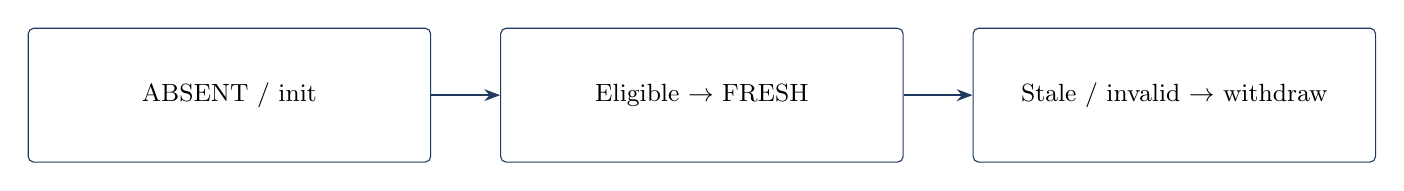
\begin{tikzpicture}\node[box,text width=49mm,minimum height=17mm] (a0) at (0.0,0) {ABSENT / init};\node[box,text width=49mm,minimum height=17mm] (a1) at (6.0,0) {Eligible $\to$ FRESH};\draw[flow] (a0.east)--(a1.west);\node[box,text width=49mm,minimum height=17mm] (a2) at (12.0,0) {Stale / invalid $\to$ withdraw};\draw[flow] (a1.east)--(a2.west);\end{tikzpicture}}{Planned WBR semantics; OS INIT/FRESH/HOLD/FAILSAFE is a separate implementation.}
\vfill\takeaway{Why WBR cares: a heartbeat proves liveness, not freshness or physical validity.}
\note{base/main-v4-91p.tex; base/main.tex Phase 8; docs/PROJECT\_STATE.md and NEXT\_GATE.md. Offline teaching synthesis; no new physical evidence.}
\end{frame}
\begin{frame}{Health envelope: check yourself}
\evidence{SOURCE-SUPPORTED planned semantics}
\deckitems{\item Worked case: sequence advances and heartbeat is current, but pose epoch stays unchanged. Is the pose FRESH?}
\vfill\takeaway{Work out your answer before turning the page.}
\note{base/main-v4-91p.tex; base/main.tex Phase 8; docs/PROJECT\_STATE.md and NEXT\_GATE.md. Offline teaching synthesis; no new physical evidence.}
\end{frame}
\begin{frame}{Health envelope: answer}
\evidence{SOURCE-SUPPORTED planned semantics}
\deckitems{\item Not from that evidence. The receiver must bound source age; repeated transmission does not rejuvenate an old estimate.\item Test stale epochs, NaN, wrong frames, duplicates, clock wrap and resets in N6 fixtures before N7.}
\vfill\takeaway{Explain the evidence that would distinguish the two cases.}
\note{base/main-v4-91p.tex; base/main.tex Phase 8; docs/PROJECT\_STATE.md and NEXT\_GATE.md. Offline teaching synthesis; no new physical evidence.}
\end{frame}
\begin{frame}{N7: keep the control path independent}
\evidence{KNOWN method / WBR qualification OPEN}
\deckitems{\item The receiver may admit reviewed optional navigation data when its envelope is eligible.\item STM32 body IMU, local estimation, watchdog and control limits keep authority when the Pi disappears.\item First test a receiver bench without actuation, then separately approved controlled integration.}
\par\medskip \coursefigure{b2-boundary}{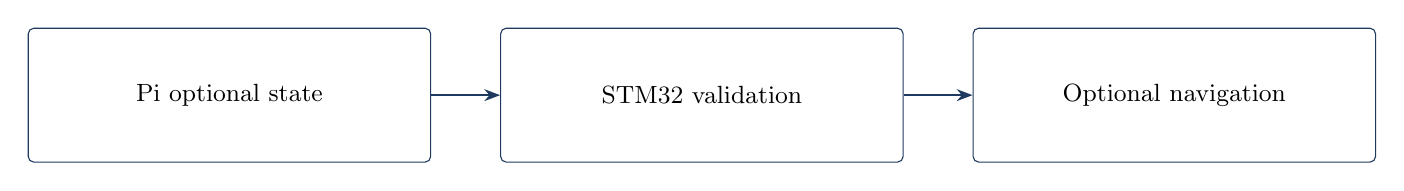
\begin{tikzpicture}\node[box,text width=49mm,minimum height=17mm] (a0) at (0.0,0) {Pi optional state};\node[box,text width=49mm,minimum height=17mm] (a1) at (6.0,0) {STM32 validation};\draw[flow] (a0.east)--(a1.west);\node[box,text width=49mm,minimum height=17mm] (a2) at (12.0,0) {Optional navigation};\draw[flow] (a1.east)--(a2.west);\end{tikzpicture}}{Independent local body sensing $\to$ balance $\to$ motor limits remains controller-owned.}
\vfill\takeaway{Bench packets cannot establish physical balancing or a safe fallback time.}
\note{base/main-v4-91p.tex; base/main.tex Phase 8; docs/PROJECT\_STATE.md and NEXT\_GATE.md. Offline teaching synthesis; no new physical evidence.}
\end{frame}
\begin{frame}{UART: worked serialization floors}
\evidence{CALCULATED from source framing}
\deckitems{\item WBR bench request/reply wire lengths imply ≈3.65 ms at 115200 baud.\item CN E7 sends chunked images; 30 kB plus framing is 30,510 UART bytes.\item At 115200 8N1, the E7 ingress line-time floor is ≈2.648 s.}
\par\medskip \[T_{wire}=\frac{10\,N_{bytes}}{\mathrm{baud}}\quad\text{(8N1)}\]
\vfill\takeaway{UART image ingress and small supervisory messages have different budgets.}
\note{Link step 9c expects request ≈2210 us and reply ≈1430 us. CN E7\_DESIGN.md includes 17-byte overhead per 1024-byte chunk. These are floors, not measured RTT.}
\end{frame}
\begin{frame}{CN/OS supervisor states and recovery}
\evidence{SOURCE-SUPPORTED OS integration / hardware UNTESTED}
\begin{tabular}{@{}L{52mm}L{128mm}@{}}\toprule
\textbf{State} & \textbf{Source-defined behavior}\\\midrule
INIT = 0 & Readiness incomplete; fresh local and network evidence required.\\[6pt]
FRESH = 1 & All required liveness, age and validity checks healthy.\\[6pt]
HOLD = 2 & Results stale; can recover when all checks become healthy.\\[6pt]
FAILSAFE = 3 & Latched; board port requires reset, then new readiness.\\[6pt]\bottomrule\end{tabular}\vfill\takeaway{Stop results with heartbeat alive to show HOLD before FAILSAFE.}
\note{Original OS protocol v1 names states but does not define transition thresholds. Newer OS-wt-cn docs/CN\_INTEGRATION.md: heartbeat timeout 100 ms, result/network HOLD 200 ms, FAILSAFE 500 ms, 1 s healthy rearm API, 5 ms transit allowance; provisional defaults, not WBR safety budgets.}
\end{frame}
\begin{frame}{Link and supervision: common mistake and check yourself}
\evidence{KNOWN method}
\deckitems{\item Mistake: stop the whole Pi bridge and expect HOLD$\to$FAILSAFE.\item Local heartbeat loss triggers FAILSAFE at 100 ms; network stale-data path is separate.\item Question: do new packets automatically recover latched FAILSAFE?}
\vfill\takeaway{Two fault injections test two mechanisms; record state and reason.}
\note{Answer: no. HOLD can return to FRESH; latched FAILSAFE needs explicit local rearm API after health, or board reset on this port. Neither link-bench NO\_LINK nor CN/OS host tests prove WBR physical independence.}
\end{frame}
\begin{frame}{Link and supervision: answer}
\evidence{KNOWN method / WBR qualification OPEN}
\deckitems{\item No. New packets do not automatically clear latched FAILSAFE.\item HOLD can recover when checks become healthy; this OS board port requires reset for FAILSAFE, then new readiness.}
\vfill\takeaway{Use this answer to check the reasoning on the preceding page.}
\note{base/main-v4-91p.tex; base/main.tex Phase 8; docs/PROJECT\_STATE.md and NEXT\_GATE.md. Offline teaching synthesis; no new physical evidence.}
\end{frame}
\begin{frame}{Bottom-up diagnosis: find the earliest failed layer}
\evidence{KNOWN method / WBR qualification OPEN}
\deckitems{\item Start with power/cooling, own USB branch, access and raw stream identity.\item Then inspect clocks, wrapper graph/QoS, recording/replay and conversion fidelity.\item Only after calibration and input coverage pass should you inspect ORB state and trajectory metrics.}
\par\medskip \coursefigure{b2-diagnosis}{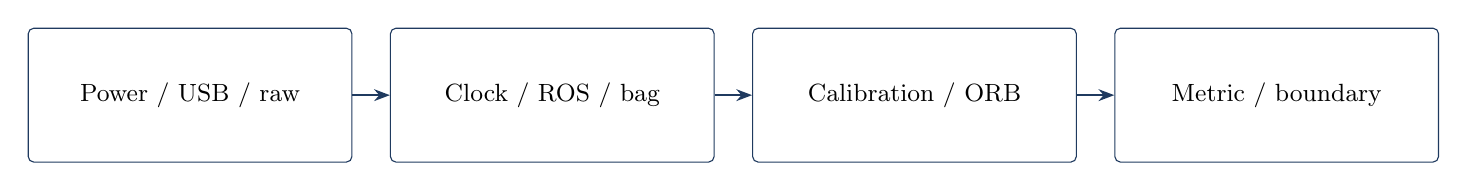
\begin{tikzpicture}\node[box,text width=39mm,minimum height=17mm] (a0) at (0.0,0) {Power / USB / raw};\node[box,text width=39mm,minimum height=17mm] (a1) at (4.6,0) {Clock / ROS / bag};\draw[flow] (a0.east)--(a1.west);\node[box,text width=39mm,minimum height=17mm] (a2) at (9.2,0) {Calibration / ORB};\draw[flow] (a1.east)--(a2.west);\node[box,text width=39mm,minimum height=17mm] (a3) at (13.799999999999999,0) {Metric / boundary};\draw[flow] (a2.east)--(a3.west);\end{tikzpicture}}{A failed earlier layer stops downstream acceptance; independent work can continue.}
\vfill\takeaway{Why WBR cares: changing a late-stage parameter can conceal an upstream acquisition defect.}
\note{base/main-v4-91p.tex; base/main.tex Phase 8; docs/PROJECT\_STATE.md and NEXT\_GATE.md. Offline teaching synthesis; no new physical evidence.}
\end{frame}
\begin{frame}{Diagnosis: symptom, evidence, next action}
\evidence{SOURCE-SUPPORTED contract / gate OPEN}
\begin{tabular}{@{}L{84mm}L{96mm}@{}}\toprule
\textbf{Symptom} & \textbf{Inspect before changing anything}\\\midrule
Images work, motion is silent & HID/IIO access, raw stream selection and exact topic graph.\\[6pt]
Bag gaps appear only under recording load & Durable-write batches, mount identity and queue events.\\[6pt]
Depth scale or gravity looks wrong & Frame direction, units, rectification and timestamps.\\[6pt]
Offline works, live output ages & Queue wait, executor scheduling, CPU clock and loaded power.\\[6pt]\bottomrule\end{tabular}\vfill\takeaway{Common mistake: reinstall or tune SLAM before preserving the discriminating evidence.}
\note{base/main-v4-91p.tex; base/main.tex Phase 8; docs/PROJECT\_STATE.md and NEXT\_GATE.md. Offline teaching synthesis; no new physical evidence.}
\end{frame}
\begin{frame}{Bottom-up diagnosis: check yourself}
\evidence{KNOWN method / illustrative question}
\deckitems{\item A 15 s RAM take is clean but a card take develops 2 s gaps. Which next check separates hypotheses?}
\vfill\takeaway{Work out your answer before turning the page.}
\note{base/main-v4-91p.tex; base/main.tex Phase 8; docs/PROJECT\_STATE.md and NEXT\_GATE.md. Offline teaching synthesis; no new physical evidence.}
\end{frame}
\begin{frame}{Bottom-up diagnosis: answer}
\evidence{KNOWN method / illustrative question}
\deckitems{\item Inspect sustained durable-write batches and queue/backpressure logs under the same source load.\item The observation supports a storage-path hypothesis; it does not prove the sensor is faulty or the card is qualified.}
\vfill\takeaway{Explain the evidence that would distinguish the two cases.}
\note{base/main-v4-91p.tex; base/main.tex Phase 8; docs/PROJECT\_STATE.md and NEXT\_GATE.md. Offline teaching synthesis; no new physical evidence.}
\end{frame}
\begin{frame}{Engineering choices: what evidence would change them?}
\evidence{SOURCE-SUPPORTED contract / gate OPEN}
\begin{tabular}{@{}L{90mm}L{90mm}@{}}\toprule
\textbf{Current choice} & \textbf{Evidence needed to reconsider}\\\midrule
Native Pi runtime; direct USB3 cable & Equivalent physical gates plus a packaging/topology benefit.\\[6pt]
Upstream EuRoC $\to$ offline camera $\to$ live & Matched-data equivalence before adding a wrapper or live path.\\[6pt]
Measured calibration/noise before tuning & Import/model support and held-out residual improvement.\\[6pt]
Defer wheel-odometry fusion & Synchronized geometry, covariance meaning and slip evidence.\\[6pt]\bottomrule\end{tabular}\vfill\takeaway{Add complexity to address a measured failure; keep the comparison controlled.}
\note{v4 §6.1–6.3; Phase-8 direct SDK versus planned ROS distinction. Docker remains an offline Kalibr tool, not a proven Pi acquisition fix.}
\end{frame}
\begin{frame}{Reproduction: the evidence packet is the output}
\evidence{KNOWN method / WBR qualification OPEN}
\deckitems{\item Keep raw data, device/boot identity, exact argv, settings and binary/library/source hashes.\item Link every derivative to its immutable inputs; preserve failures and actual review receipts.\item Separate an automatic capture result, a human review and a sealed acceptance decision.}
\par\medskip \coursefigure{b2-reproduce}{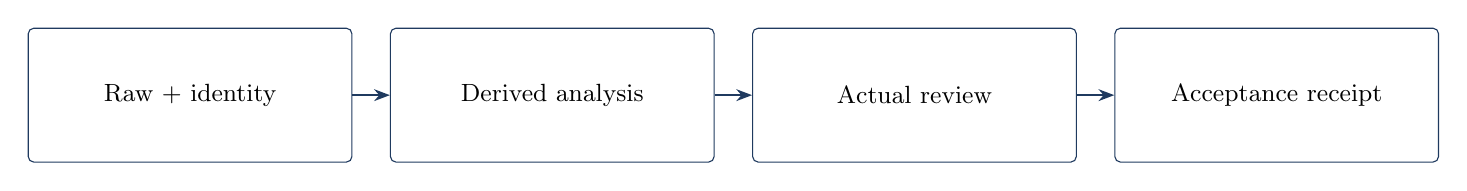
\begin{tikzpicture}\node[box,text width=39mm,minimum height=17mm] (a0) at (0.0,0) {Raw + identity};\node[box,text width=39mm,minimum height=17mm] (a1) at (4.6,0) {Derived analysis};\draw[flow] (a0.east)--(a1.west);\node[box,text width=39mm,minimum height=17mm] (a2) at (9.2,0) {Actual review};\draw[flow] (a1.east)--(a2.west);\node[box,text width=39mm,minimum height=17mm] (a3) at (13.799999999999999,0) {Acceptance receipt};\draw[flow] (a2.east)--(a3.west);\end{tikzpicture}}{No prefilled approval and no editing deployed tools in place.}
\vfill\takeaway{A complete packet lets another person recompute the claim without repeating the lab.}
\note{base/main-v4-91p.tex; base/main.tex Phase 8; docs/PROJECT\_STATE.md and NEXT\_GATE.md. Offline teaching synthesis; no new physical evidence.}
\end{frame}
\begin{frame}{Bounded analysis tickets: one uncertainty at a time}
\evidence{KNOWN workflow / future execution OPEN}
\deckitems{\item State one question, allowed files/hosts/actions and a fixed evidence input.\item Require a discriminating check, retained outputs and explicit STOP conditions.\item The owner accepts gate and safety decisions; an analysis tool cannot manufacture missing hardware evidence.}
\vfill\takeaway{Example ticket: audit one take’s timestamp order and explain every rejection.}
\note{v4 §4.18. This is teaching content; no subagents or runtime work were invoked.}
\end{frame}
\begin{frame}{Historical evidence: keep unit and date attached}
\evidence{MEASURED archived / all gates OPEN}
\deckitems{\item September x86/VM USB2 and later Pi 5000M$\to$480M behavior explain transport risks.\item A historical 105 s capture did not complete N2; old-camera evidence does not transfer to this unit.\item Phase 8 adds the 8 GB boot, card gaps, clean short RAM take and interrupted crash-repair rebuild.}
\vfill\takeaway{Historical progress explains the next test; it never silently becomes current acceptance.}
\note{v4 §7.1–7.3; Phase-8 §7 and docs/PROJECT\_STATE. Later lab report of still replay is dated separately.}
\end{frame}
\begin{frame}{Current gaps: what would close each one?}
\evidence{OPEN / dated source synthesis}
\begin{tabular}{@{}L{88mm}L{92mm}@{}}\toprule
\textbf{Gap} & \textbf{Next evidence}\\\midrule
N0–N3 platform/new-unit input & Loaded healthy power, qualified storage, fresh strict receipts.\\[6pt]
N4A known dataset & Stable-power repeats and reviewed accuracy/continuity budgets.\\[6pt]
N4B/C camera estimation & Stereo/time/calibration audit, motion replay, then live counters.\\[6pt]
N5–N7 measurement / boundary & Raw event series, semantic fixtures, approved controller traces.\\[6pt]\bottomrule\end{tabular}\vfill\takeaway{The active project gate remains N3; diagnostic work does not replace it.}
\note{base/main-v4-91p.tex; base/main.tex Phase 8; docs/PROJECT\_STATE.md and NEXT\_GATE.md. Offline teaching synthesis; no new physical evidence.}
\end{frame}
\begin{frame}{Conditional roadmap: proceed on evidence}
\evidence{SOURCE-SUPPORTED conditional plan / no gate PASS}
\deckitems{\item Refresh stable N0, renew N1 and finish exact N2/N3 before qualified camera claims.\item Phase-8 diagnostic roadmap: complete the repair build, record a 100 s RAM motion take, replay/plot, then live diagnostic.\item The later source reports only a clean still replay without a map; motion and live remain OPEN.}
\par\medskip \coursefigure{b2-roadmap}{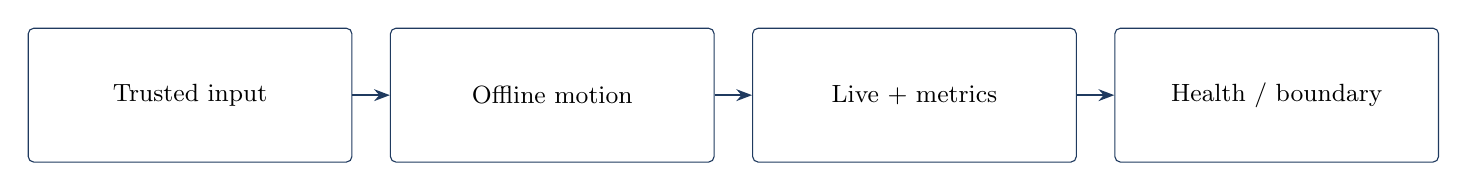
\begin{tikzpicture}\node[box,text width=39mm,minimum height=17mm] (a0) at (0.0,0) {Trusted input};\node[box,text width=39mm,minimum height=17mm] (a1) at (4.6,0) {Offline motion};\draw[flow] (a0.east)--(a1.west);\node[box,text width=39mm,minimum height=17mm] (a2) at (9.2,0) {Live + metrics};\draw[flow] (a1.east)--(a2.west);\node[box,text width=39mm,minimum height=17mm] (a3) at (13.799999999999999,0) {Health / boundary};\draw[flow] (a2.east)--(a3.west);\end{tikzpicture}}{Dates and a successful launch do not advance a gate.}
\vfill\takeaway{N4A can proceed independently; N6 review and N7 authorization remain separate.}
\note{base/main-v4-91p.tex; base/main.tex Phase 8; docs/PROJECT\_STATE.md and NEXT\_GATE.md. Offline teaching synthesis; no new physical evidence.}
\end{frame}
\begin{frame}{Conclusion: explain the system aloud}
\evidence{KNOWN method / WBR qualification OPEN}
\deckitems{\item Describe how paired pixels and covered raw IMU become a pose in a named frame and epoch.\item Explain why geometry, noise, clocks, queues and storage each need separate evidence.\item Describe how stale, invalid or reset perception is withdrawn while STM32 retains local control.}
\vfill\takeaway{Understanding means predicting both the useful output and the failure path.}
\note{base/main-v4-91p.tex; base/main.tex Phase 8; docs/PROJECT\_STATE.md and NEXT\_GATE.md. Offline teaching synthesis; no new physical evidence.}
\end{frame}
\begin{frame}{Lecture recap: check yourself}
\evidence{KNOWN method / illustrative question}
\deckitems{\item You have a plausible trajectory, clean exit and a live heartbeat. Which three checks still guard a receiver?}
\vfill\takeaway{Work out your answer before turning the page.}
\note{base/main-v4-91p.tex; base/main.tex Phase 8; docs/PROJECT\_STATE.md and NEXT\_GATE.md. Offline teaching synthesis; no new physical evidence.}
\end{frame}
\begin{frame}{Lecture recap: answer}
\evidence{KNOWN method / illustrative question}
\deckitems{\item Check frame/session/reset validity, finite supported state and a conservative source-age bound.\item Those checks complement acquisition and calibration evidence; a plausible path is only one part of the chain.}
\vfill\takeaway{Explain the evidence that would distinguish the two cases.}
\note{base/main-v4-91p.tex; base/main.tex Phase 8; docs/PROJECT\_STATE.md and NEXT\_GATE.md. Offline teaching synthesis; no new physical evidence.}
\end{frame}
\begin{frame}{Lab operating contract}
\evidence{ASSUMED time budget / SOURCE-SUPPORTED stop rules}
\deckitems{\item Each supervised session is capped at 150 min; first failure consumes the retry buffer.\item No build, install, card clone or persistent network change belongs in these sessions.\item The 30 min warm-up and Allan take ($\geq$4 h provisional; 15–24 h preferred) happen at home.}
\vfill\takeaway{Stop at the time cap; leave skipped work OPEN.}
\note{Study synthesis from base/main-v4-91p.tex, updated against base/main.tex. No new physical evidence; every gate remains OPEN.}
\end{frame}
\begin{frame}{Packing checklist}
\evidence{SOURCE-SUPPORTED packing / availability to verify}
\deckitems{\item 8 GB Pi + qualified 128 GB card + 27 W supply; 4 GB Pi + own supply for CN.\item D435i/cable, Ethernet, Mac/power, rigid measured AprilGrid, ruler/calipers, tape.\item F446RE, Mac USB cable, 3 jumpers; optional analyzer; prepared firmware and tools.}
\vfill\takeaway{Pack distinct link-bench and OS-supervisor firmware with hashes.}
\note{Study synthesis from base/main-v4-91p.tex, updated against base/main.tex. No new physical evidence; every gate remains OPEN.}
\end{frame}
\begin{frame}{Stop rules: the earliest failed layer wins}
\evidence{SOURCE-SUPPORTED prerequisites / ASSUMED one-retry policy}
\deckitems{\item New live power fault, reboot, USB <5000M or data reversal: stop acquisition.\item At a missing tool, unknown device identity or unverified command: stop that branch.\item One corrected retry with a new ID; then defer to Session 2 or home preparation.}
\vfill\takeaway{Do not tune SLAM, erase failed takes or relax thresholds to hide sensor faults.}
\note{Study synthesis from base/main-v4-91p.tex, updated against base/main.tex. No new physical evidence; every gate remains OPEN.}
\end{frame}
\begin{frame}{Shell variables used in the lab}
\evidence{SOURCE-SUPPORTED shell bindings / chosen deployment paths}
\begin{tabular}{@{}L{60mm}L{120mm}@{}}\toprule
\textbf{Variable / binding} & \textbf{Plain meaning}\\\midrule
\$HOME & The shell’s existing home folder; never change it.\\[6pt]
\$GATE & Prepared complete gate bundle: \textasciitilde{}/wbr-runtime/study-gates.\\[6pt]
\$RUN & This session’s small logs/receipts: \textasciitilde{}/wbr-evidence/study-S1-20261018.\\[6pt]
\$DATA & This session’s take root: \textasciitilde{}/wbr-takes/study-S1-20261018.\\[6pt]
\$STUDY & Prepared copy of this package: \textasciitilde{}/wbr-runtime/study-docs.\\[6pt]\bottomrule\end{tabular}\vfill\takeaway{Repeat bindings in each named terminal; use fresh actual session and take IDs.}
\note{Study synthesis from base/main-v4-91p.tex, updated against base/main.tex. No new physical evidence; every gate remains OPEN.}
\end{frame}
\begin{frame}{Shell variables: take and terminal identity}
\evidence{SOURCE-SUPPORTED shell bindings / chosen deployment paths}
\begin{tabular}{@{}L{60mm}L{120mm}@{}}\toprule
\textbf{Variable / binding} & \textbf{Plain meaning}\\\midrule
\$ID & Fresh take name, such as S-ROS-01 or C1-ROS-01; repeat in every terminal.\\[6pt]
\$TOPICS & Bash array of explicit topics; define in the recorder shell before use.\\[6pt]
\$TAKE & Completed native take name used by the handoff copy loop.\\[6pt]
\$PORT & Actual checked UART device, such as /dev/ttyAMA0; not a guessed port.\\[6pt]
\$WBR\_HOST & Prepared demo SSH target richard@192.168.50.2; verify against inventory.\\[6pt]\bottomrule\end{tabular}\vfill\takeaway{Repeat bindings in each named terminal; use fresh actual session and take IDs.}
\note{Study synthesis from base/main-v4-91p.tex, updated against base/main.tex. No new physical evidence; every gate remains OPEN.}
\end{frame}
\begin{frame}{Shell variables: home analysis paths}
\evidence{SOURCE-SUPPORTED shell bindings / chosen deployment paths}
\begin{tabular}{@{}L{60mm}L{120mm}@{}}\toprule
\textbf{Variable / binding} & \textbf{Plain meaning}\\\midrule
\$ARCH & Copied Mac session root under \textasciitilde{}/Desktop/Research/wbr-data/.\\[6pt]
\$BAG & An actual finalized ROS bag directory, not a native SDK file.\\[6pt]
\$NATIVE & An actual finalized native take/ folder containing stereo\_imu.db3.\\[6pt]
\$DERIVED & Fresh output parent for analysis; keep it separate from raw takes.\\[6pt]
\$TARGET & Measured target YAML at the explicit H4 path; nominal dimensions are insufficient.\\[6pt]\bottomrule\end{tabular}\vfill\takeaway{Repeat bindings in each named terminal; use fresh actual session and take IDs.}
\note{Study synthesis from base/main-v4-91p.tex, updated against base/main.tex. No new physical evidence; every gate remains OPEN.}
\end{frame}
\begin{frame}{Shell variables: ORB and CN bindings}
\evidence{SOURCE-SUPPORTED shell bindings / chosen deployment paths}
\begin{tabular}{@{}L{60mm}L{120mm}@{}}\toprule
\textbf{Variable / binding} & \textbf{Plain meaning}\\\midrule
\$ORB\_DIR / \$TAKE\_DIR & Prepared ORB root / audited exported sequence used in H6.\\[6pt]
\$SETTINGS\_FILE / \$LD\_LIBRARY\_PATH & Reviewed ORB YAML / runtime library search list from H6.\\[6pt]
\$WIFI\_B & Pi B’s measured Wi-Fi IPv4 address; Pi A must route to it over wlan0.\\[6pt]
\$CN\_CLIENT\_SSH / \$CN\_EDGE\_SSH & Actual client/edge user@host bindings entered during S2 archive.\\[6pt]\bottomrule\end{tabular}\vfill\takeaway{Repeat bindings in each named terminal; use fresh actual session and take IDs.}
\note{Study synthesis from base/main-v4-91p.tex, updated against base/main.tex. No new physical evidence; every gate remains OPEN.}
\end{frame}
\begin{frame}{Shell variables: repeat bindings in each terminal}
\evidence{SOURCE-SUPPORTED shell bindings / chosen deployment paths}
\begin{tabular}{@{}L{60mm}L{120mm}@{}}\toprule
\textbf{Variable / binding} & \textbf{Plain meaning}\\\midrule
Session 2 RUN / DATA & Use study-S2-20261019 as shown in S2.0; dates are examples, not observations.\\[6pt]
ROS\_DOMAIN\_ID=42 / 43 & Environment: localhost live acquisition / isolated home replay.\\[6pt]
ROS\_LOCALHOST\_ONLY=1 & Environment: keep the ROS graph on the current machine.\\[6pt]
STUDY versus \textasciitilde{}/CN & STUDY holds study configs; \textasciitilde{}/CN is the separately prepared CN checkout.\\[6pt]\bottomrule\end{tabular}\vfill\takeaway{Repeat bindings in each named terminal; use fresh actual session and take IDs.}
\note{Study synthesis from base/main-v4-91p.tex, updated against base/main.tex. No new physical evidence; every gate remains OPEN.}
\end{frame}
\begin{frame}{Session 1 map: stop at the earliest failed prerequisite}
\evidence{ASSUMED session decision map}
\coursefigure{b2-map-1}{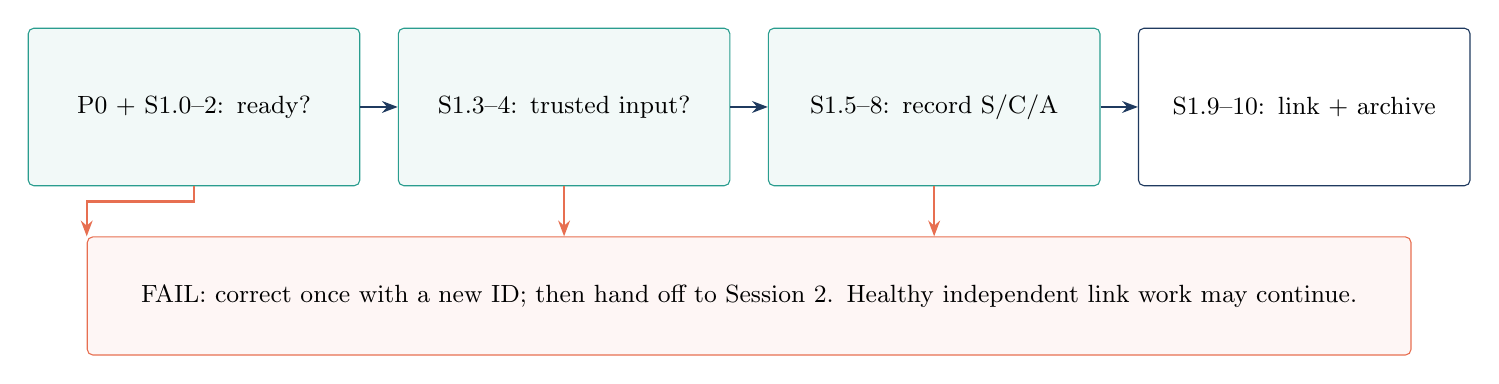
\begin{tikzpicture}\node[box,draw=teal,fill=teal!6,text width=40mm,minimum height=20mm] (m0) at (0.0,0) {P0 + S1.0–2: ready?};\node[box,draw=teal,fill=teal!6,text width=40mm,minimum height=20mm] (m1) at (4.7,0) {S1.3–4: trusted input?};\draw[flow] (m0.east)--(m1.west);\node[box,draw=teal,fill=teal!6,text width=40mm,minimum height=20mm] (m2) at (9.4,0) {S1.5–8: record S/C/A};\draw[flow] (m1.east)--(m2.west);\node[box,text width=40mm,minimum height=20mm] (m3) at (14.100000000000001,0) {S1.9–10: link + archive};\draw[flow] (m2.east)--(m3.west);\node[box,draw=fault,fill=fault!6,text width=166mm,minimum height=15mm] (stop) at (7.05,-2.4) {FAIL: correct once with a new ID; then hand off to Session 2. Healthy independent link work may continue.};\draw[faultflow] (m0.south)--(0,-1.2)-|(stop.north west);\draw[faultflow] (m1.south)--(m1.south|-stop.north);\draw[faultflow] (m2.south)--(m2.south|-stop.north);\end{tikzpicture}}{YES follows the top arrows; failed readiness follows the lower branch. Stop at 150 minutes.}\vfill\takeaway{Read the step card before its commands. Preserve failed and skipped work as evidence.}
\note{BRIEF2.md; matching timelines and step criteria. No operational command changed.}
\end{frame}
\begin{frame}{Session 1 timeline: 150 min maximum}
\evidence{ASSUMED wall-time budget}
\begin{tabular}{@{}L{63mm}L{117mm}@{}}\toprule
\textbf{Elapsed} & \textbf{Task / exit artifact}\\\midrule
0–15 / 15–30 min & S1.0–2: setup, power, storage/USB identity.\\[6pt]
30–55 / 55–75 min & S1.3–4: N2 stages/review; N3 audit/record-replay.\\[6pt]
75–110 / 110–125 min & S1.5–7: ROS S/C takes; native replicas only if ready.\\[6pt]
125–140 / 140–150 min & S1.8–10: A pilot plan, link bench, verified handoff.\\[6pt]\bottomrule\end{tabular}\vfill\takeaway{N3 unresolved at minute 75 means calibration qualification is deferred.}
\note{Study synthesis from base/main-v4-91p.tex, updated against base/main.tex. No new physical evidence; every gate remains OPEN.}
\end{frame}
\begin{frame}{Before lab: prepare, do not improvise}
\evidence{SOURCE-SUPPORTED runbook / readiness OPEN}
\deckitems{\item Owner-authorized transfer/deployment, card setup and any builds happen beforehand.\item Gate bundle, wrapper, ROS CLI, native recorder, Kalibr image and CN files must exist.\item The strict card exception needs a reviewed sustained-write receipt; capacity is insufficient.}
\vfill\takeaway{An unready prerequisite becomes a documented skipped step.}
\note{Latest lab runbook requires owner phrase transfer before clone/deployment/write tests. The study builder performs none. No new permission is being requested for document generation.}
\end{frame}
\begin{frame}{P0 | Bind prepared paths and verify tools}
\evidence{SOURCE-SUPPORTED procedure / execution OPEN}
\textbf{Goal / why:} Check the prepared tools and name the output folders before connecting hardware, so every later command has a known location.\par\medskip\textbf{Physical setup:} On the Mac, open the canonical WBR checkout. On each Pi terminal, source Jazzy and repeat the path bindings. Keep all camera programs stopped.\par\medskip\textbf{What you see:} The help command lists the demo interface. Each file test returns without an error; the new RUN and DATA folders exist.
\note{Canonical AGENTS.md; archived PHASE\_A\_RUNBOOK.md; demo.sh --help; docs/D435I\_CALIBRATION\_PLAN.md storage exception. study-gates is an explicitly chosen pre-lab deployment location, not a claimed existing runtime path. It must contain the full checksummed archived bundle; do not copy individual gate files. Session date/IDs are operator run IDs, not claims of capture on 18 Oct. Repeat environment bindings in each Pi terminal. DATA is a dedicated directory on the qualified 128 GB slot card; record actual findmnt/lsblk identity.}
\end{frame}
\begin{frame}{P0 | Decision, recovery and files}
\evidence{SOURCE-SUPPORTED procedure / execution OPEN}
\textbf{PASS / FAIL:} Continue only if every required file is present and the chosen output folders are fresh. A missing file leaves this branch OPEN.\par\medskip\textbf{If FAIL:} Stop this branch and prepare the missing dependency at home. Do not install tools or guess another script during the session.\par\medskip\textbf{Take these files home:} Keep Pi logs in RUN and takes in DATA. Keep the source revision and dirty-file record with the Mac session archive.
\note{Canonical AGENTS.md; archived PHASE\_A\_RUNBOOK.md; demo.sh --help; docs/D435I\_CALIBRATION\_PLAN.md storage exception. study-gates is an explicitly chosen pre-lab deployment location, not a claimed existing runtime path. It must contain the full checksummed archived bundle; do not copy individual gate files. Session date/IDs are operator run IDs, not claims of capture on 18 Oct. Repeat environment bindings in each Pi terminal. DATA is a dedicated directory on the qualified 128 GB slot card; record actual findmnt/lsblk identity.}
\end{frame}
\begin{frame}[fragile]{P0 | Mac / before lab (1/2)}
\evidence{SOURCE-SUPPORTED procedure / execution OPEN}
\begin{lstlisting}
cd ~/Desktop/Research/wbr-perception-phase1-runtime
export WBR_HOST=richard@192.168.50.2
bash experiments/2026-10-15-demo-day/demo.sh --help
git rev-parse HEAD
git status --short
\end{lstlisting}
\vfill\takeaway{Use the checks and failure branch on the preceding P0 step card.}
\note{Canonical AGENTS.md; archived PHASE\_A\_RUNBOOK.md; demo.sh --help; docs/D435I\_CALIBRATION\_PLAN.md storage exception.}
\end{frame}
\begin{frame}[fragile]{P0 | Pi / each shell (2/2)}
\evidence{SOURCE-SUPPORTED procedure / execution OPEN}
\begin{lstlisting}
source /opt/ros/jazzy/setup.bash
export GATE="$HOME/wbr-runtime/study-gates"
export RUN="$HOME/wbr-evidence/study-S1-20261018"
export DATA="$HOME/wbr-takes/study-S1-20261018"
# Prepared, reviewed 128 GB data-directory exception.
mkdir -p "$RUN" "$DATA"
test -f "$GATE/phase_gate.py"
test -f "$GATE/n3_record.py"
test -f "$GATE/n3_bag.py"
export ROS_DOMAIN_ID=42 ROS_LOCALHOST_ONLY=1
\end{lstlisting}
\vfill\takeaway{Use the checks and failure branch on the preceding P0 step card.}
\note{Canonical AGENTS.md; archived PHASE\_A\_RUNBOOK.md; demo.sh --help; docs/D435I\_CALIBRATION\_PLAN.md storage exception.}
\end{frame}
\begin{frame}{S1.0 | Set up and make the evidence manifest}
\evidence{SOURCE-SUPPORTED procedure / execution OPEN}
\textbf{Goal / why:} Document the physical assembly before testing it, so a result can be traced to the board, supply, cable and storage actually used.\par\medskip\textbf{Physical setup:} Secure the Pi and camera cable against pulling. Use the direct USB3 cable and connect power last. Camera access requires the owner’s CAMERA AVAILABLE instruction.\par\medskip\textbf{What you see:} The identity file shows the running kernel and resolved data mount. Your notebook identifies the supply, cooler, board, card, target and room.
\note{Latest lab runbook steps 0–3; calibration plan per-take manifest. Standard read-only Linux/macOS commands. Copy /tmp/study-source-* and study-config.sha256 into the final session archive before /tmp cleanup. Record actual tool/binary/config hashes, wrapper version, SDK version, serials separately and notes on any dirty sources; a Git hash alone is insufficient.}
\end{frame}
\begin{frame}{S1.0 | Decision, recovery and files}
\evidence{SOURCE-SUPPORTED procedure / execution OPEN}
\textbf{PASS / FAIL:} Continue when every identity field is recorded or explicitly marked UNKNOWN, and the process list shows no competing camera owner.\par\medskip\textbf{If FAIL:} Correct cabling or process ownership first. Record any missing identity; use a fresh run folder rather than overwriting earlier evidence.\par\medskip\textbf{Take these files home:} Save RUN/identity.txt and processes-before.txt. Retain the Mac source/config hash files and measured-target notes in the same session archive.
\note{Latest lab runbook steps 0–3; calibration plan per-take manifest. Standard read-only Linux/macOS commands. Copy /tmp/study-source-* and study-config.sha256 into the final session archive before /tmp cleanup. Record actual tool/binary/config hashes, wrapper version, SDK version, serials separately and notes on any dirty sources; a Git hash alone is insufficient.}
\end{frame}
\begin{frame}[fragile]{S1.0 | Pi / control (1/2)}
\evidence{SOURCE-SUPPORTED procedure / execution OPEN}
\begin{lstlisting}
uptime > "$RUN/identity.txt"
uname -a >> "$RUN/identity.txt"
findmnt -T "$DATA" >> "$RUN/identity.txt"
lsblk -o NAME,SIZE,MODEL,FSTYPE,UUID,MOUNTPOINTS \
  >> "$RUN/identity.txt"
ps -eo pid,args > "$RUN/processes-before.txt"
\end{lstlisting}
\vfill\takeaway{Use the checks and failure branch on the preceding S1.0 step card.}
\note{Latest lab runbook steps 0–3; calibration plan per-take manifest. Standard read-only Linux/macOS commands.}
\end{frame}
\begin{frame}[fragile]{S1.0 | Mac / canonical checkout (2/2)}
\evidence{SOURCE-SUPPORTED procedure / execution OPEN}
\begin{lstlisting}
git rev-parse HEAD > /tmp/study-source-git.txt
git status --short > /tmp/study-source-dirty.txt
shasum -a 256 calibration/lab/config/*.yaml \
  calibration/aprilgrid/*.yaml > /tmp/study-config.sha256
\end{lstlisting}
\vfill\takeaway{Use the checks and failure branch on the preceding S1.0 step card.}
\note{Latest lab runbook steps 0–3; calibration plan per-take manifest. Standard read-only Linux/macOS commands.}
\end{frame}
\begin{frame}{S1.1 | Power and storage preflight}
\evidence{SOURCE-SUPPORTED procedure / execution OPEN}
\textbf{Goal / why:} Rule out the two observed bottlenecks, weak power and slow storage, before collecting new sensor data.\par\medskip\textbf{Physical setup:} Use the 8 GB Pi with its 27 W supply and cooling. Point DATA at the prepared, qualified 128 GB data directory and have its write receipt available.\par\medskip\textbf{What you see:} The commands print raw power flags, rail voltage, temperature, available memory and disk space. A healthy power example is throttled=0x0.
\note{base/main.tex N0 table; calibration plan storage/power requirements; lab runbook telemetry. ASSUMED card qualification: test file larger than the largest take and for at least its duration, sustained $\geq$27.6 MB/s; free $\geq$2$\times$ planned take plus OS reserve. Native script uses extra RAM/disk reserves. The archived external-storage gate runner does not accept the card policy by default; that is a real N3 tooling blocker. A clone/post-boot 4 GiB speed test is not equivalent qualification. Historical latched bits are retained; strict gates still require zero.}
\end{frame}
\begin{frame}{S1.1 | Decision, recovery and files}
\evidence{SOURCE-SUPPORTED procedure / execution OPEN}
\textbf{PASS / FAIL:} N0 requires flags 0x0, temperature below 75$^\circ$C and available memory $\geq$512 MiB. The card exception proposes sustained writes $\geq$27.6 MB/s; this margin is ASSUMED.\par\medskip\textbf{If FAIL:} Stop acquisition after a power fault or reboot. Check supply, cable and cooling, then storage identity and write evidence. An unqualified volume cannot receive a qualified take.\par\medskip\textbf{Take these files home:} Keep RUN/power-before.txt and capacity.txt, the original write receipt and its hash. Record the actual free-space reserve before each take.
\note{base/main.tex N0 table; calibration plan storage/power requirements; lab runbook telemetry. ASSUMED card qualification: test file larger than the largest take and for at least its duration, sustained $\geq$27.6 MB/s; free $\geq$2$\times$ planned take plus OS reserve. Native script uses extra RAM/disk reserves. The archived external-storage gate runner does not accept the card policy by default; that is a real N3 tooling blocker. A clone/post-boot 4 GiB speed test is not equivalent qualification. Historical latched bits are retained; strict gates still require zero.}
\end{frame}
\begin{frame}[fragile]{S1.1 | Pi / control (1/1)}
\evidence{SOURCE-SUPPORTED procedure / execution OPEN}
\begin{lstlisting}
vcgencmd get_throttled | tee "$RUN/power-before.txt"
vcgencmd pmic_read_adc EXT5V_V \
  | tee -a "$RUN/power-before.txt"
vcgencmd measure_temp | tee -a "$RUN/power-before.txt"
free -h | tee "$RUN/capacity.txt"
df -B1 "$DATA" /dev/shm | tee -a "$RUN/capacity.txt"
timedatectl status > "$RUN/time-before.txt"
\end{lstlisting}
\vfill\takeaway{Use the checks and failure branch on the preceding S1.1 step card.}
\note{base/main.tex N0 table; calibration plan storage/power requirements; lab runbook telemetry.}
\end{frame}
\begin{frame}{S1.2 | USB, serial and fresh N1}
\evidence{SOURCE-SUPPORTED procedure / execution OPEN}
\textbf{Goal / why:} Prove access to the current camera on its own USB branch before asking it to stream.\par\medskip\textbf{Physical setup:} Connect the D435i directly to the Pi’s blue USB3 port. Use stable N0 power, the complete prepared GATE bundle and the owner’s camera authorization.\par\medskip\textbf{What you see:} The camera’s own lsusb branch shows at least 5000M. SDK enumeration identifies serial 317422076650 and reports firmware and the other identity fields separately.
\note{Archived PHASE\_A\_RUNBOOK.md and n1\_precheck.py; source lab enumeration procedure. Read normal-user permissions; no broad chmod. N1 expires after two hours or reboot; renew after topology/storage changes. SDK enumeration warning absence does not prove physical IMU calibration.}
\end{frame}
\begin{frame}{S1.2 | Decision, recovery and files}
\evidence{SOURCE-SUPPORTED procedure / execution OPEN}
\textbf{PASS / FAIL:} Continue only if the camera branch is $\geq$5000M and n1\_precheck exits 0 with an eligible sealed receipt. Access or kernel errors fail this check.\par\medskip\textbf{If FAIL:} At 480M, stop before SDK enumeration. Inspect cable, port and intervening topology in that order; retry once into a new output folder.\par\medskip\textbf{Take these files home:} Keep RUN/usb.txt, sdk-enumeration.txt and the entire RUN/n1 directory, including result.json and its sealed raw logs.
\note{Archived PHASE\_A\_RUNBOOK.md and n1\_precheck.py; source lab enumeration procedure. Read normal-user permissions; no broad chmod. N1 expires after two hours or reboot; renew after topology/storage changes. SDK enumeration warning absence does not prove physical IMU calibration.}
\end{frame}
\begin{frame}[fragile]{S1.2 | Pi / control (1/1)}
\evidence{SOURCE-SUPPORTED procedure / execution OPEN}
\begin{lstlisting}
lsusb -t | tee "$RUN/usb.txt"
# Only after camera branch is confirmed >=5000M:
rs-enumerate-devices > "$RUN/sdk-enumeration.txt" 2>&1
cd "$GATE"
python3 n1_precheck.py --camera-available \
  --direct-cable-confirmed --output "$RUN/n1"
\end{lstlisting}
\vfill\takeaway{Use the checks and failure branch on the preceding S1.2 step card.}
\note{Archived PHASE\_A\_RUNBOOK.md and n1\_precheck.py; source lab enumeration procedure.}
\end{frame}
\begin{frame}{S1.3 | Exact N2 acquisition: inspect each stage}
\evidence{SOURCE-SUPPORTED procedure / execution OPEN}
\textbf{Goal / why:} Prove sustained raw delivery before adding ROS or SLAM; this isolates the sensor path from later software layers.\par\medskip\textbf{Physical setup:} Keep only the native gate recorder running. Use a fresh eligible N1 receipt and the exact IR1 640$\times$480 Y8/15, gyro/200 and accel/100 profile.\par\medskip\textbf{What you see:} Run 20 s, inspect the result, then 105 s, inspect again, then the mandatory 300 s soak. Each stage writes raw CSV, image samples and one-Hz health.
\note{Archived phase\_gate.py CLI and PHASE\_A\_RUNBOOK.md exact N2 stages. These native gate samples are required historical-tooling outputs; the vendor CSV lacks domain tags and rounds motion. They cannot replace full-precision calibration takes. Native gate capture has no ROS publisher; a simultaneous ROS bag is unavailable. Preserve this explicit exception/gap instead of launching a second device owner.}
\end{frame}
\begin{frame}{S1.3 | Decision, recovery and files}
\evidence{SOURCE-SUPPORTED procedure / execution OPEN}
\textbf{PASS / FAIL:} Require IR 14.25–15.75, gyro 190–210 and accel 95–105 Hz. Image gaps must be $\leq$0.20 s and motion gaps $\leq$0.05 s, with positive steps and no missing IR frames.\par\medskip\textbf{If FAIL:} Stop at the first failure. Inspect power, USB, permissions, selected profile and timestamps in that order. Allow one corrected new-ID retry, then defer to Session 2.\par\medskip\textbf{Take these files home:} Preserve RUN/smoke, reproduction and soak in full, including capture-result.json, CSV files, SDK/kernel logs and sampled PGMs.
\note{Archived phase\_gate.py CLI and PHASE\_A\_RUNBOOK.md exact N2 stages. These native gate samples are required historical-tooling outputs; the vendor CSV lacks domain tags and rounds motion. They cannot replace full-precision calibration takes. Native gate capture has no ROS publisher; a simultaneous ROS bag is unavailable. Preserve this explicit exception/gap instead of launching a second device owner.}
\end{frame}
\begin{frame}[fragile]{S1.3 | Pi / gate bundle, stage 1 (1/2)}
\evidence{SOURCE-SUPPORTED procedure / execution OPEN}
\begin{lstlisting}
cd "$GATE"
python3 phase_gate.py n2 --camera-available --seconds 20 \
  --n1-result "$RUN/n1/result.json" \
  --output "$RUN/smoke"
\end{lstlisting}
\vfill\takeaway{Use the checks and failure branch on the preceding S1.3 step card.}
\note{Archived phase\_gate.py CLI and PHASE\_A\_RUNBOOK.md exact N2 stages.}
\end{frame}
\begin{frame}[fragile]{S1.3 | Pi / only after prior stage review (2/2)}
\evidence{SOURCE-SUPPORTED procedure / execution OPEN}
\begin{lstlisting}
python3 phase_gate.py n2 --camera-available --seconds 105 \
  --n1-result "$RUN/n1/result.json" \
  --previous "$RUN/smoke/capture-result.json" \
  --output "$RUN/reproduction"
# Review that result before issuing the next command.
python3 phase_gate.py n2 --camera-available --seconds 300 \
  --n1-result "$RUN/n1/result.json" \
  --previous "$RUN/reproduction/capture-result.json" \
  --output "$RUN/soak"
\end{lstlisting}
\vfill\takeaway{Use the checks and failure branch on the preceding S1.3 step card.}
\note{Archived phase\_gate.py CLI and PHASE\_A\_RUNBOOK.md exact N2 stages.}
\end{frame}
\begin{frame}{S1.3R | Human N2 review and acceptance}
\evidence{SOURCE-SUPPORTED procedure / execution OPEN}
\textbf{Goal / why:} Turn completed captures into an actual reviewed decision; an automatic zero exit is not human acceptance.\par\medskip\textbf{Physical setup:} Open the sampled images and unfiltered logs from all three strict N2 stages. Have the real reviewer identity, UTC time and observations ready.\par\medskip\textbf{What you see:} The review file records your actual observations and retained warnings. The acceptance command checks the sealed evidence instead of trusting a claim of success.
\note{phase\_gate.py accept-n2; PHASE\_A\_RUNBOOK.md manual review schema. Review schema strings: utc, reviewer, notes, power\_supply, cooling, scene, calibration\_provenance (verified parser field: utc, timezone-aware and $\leq$2 h old). Required true booleans: raw\_logs\_clean, images\_coherent, startup\_offsets\_explained, imu\_values\_plausible, power\_cooling\_documented, calibration\_warning\_preserved. The exact UTC field is verified in the command audit; never invent a review receipt.}
\end{frame}
\begin{frame}{S1.3R | Decision, recovery and files}
\evidence{SOURCE-SUPPORTED procedure / execution OPEN}
\textbf{PASS / FAIL:} Accept only coherent images, finite plausible motion, explained startup offsets and preserved warnings, followed by eligible acceptance output. Incomplete review leaves N2 OPEN.\par\medskip\textbf{If FAIL:} Keep the gate OPEN when any required review is missing. Do not prefill true booleans or replace a strict receipt with a diagnostic capture.\par\medskip\textbf{Take these files home:} Save RUN/review.json and RUN/n2-accepted/result.json beside all original stage directories.
\note{phase\_gate.py accept-n2; PHASE\_A\_RUNBOOK.md manual review schema. Review schema strings: utc, reviewer, notes, power\_supply, cooling, scene, calibration\_provenance (verified parser field: utc, timezone-aware and $\leq$2 h old). Required true booleans: raw\_logs\_clean, images\_coherent, startup\_offsets\_explained, imu\_values\_plausible, power\_cooling\_documented, calibration\_warning\_preserved. The exact UTC field is verified in the command audit; never invent a review receipt.}
\end{frame}
\begin{frame}[fragile]{S1.3R | Pi / after actual review (1/1)}
\evidence{SOURCE-SUPPORTED procedure / execution OPEN}
\begin{lstlisting}
python3 phase_gate.py accept-n2 --camera-available \
  --n1-result "$RUN/n1/result.json" \
  --smoke "$RUN/smoke/capture-result.json" \
  --reproduction "$RUN/reproduction/capture-result.json" \
  --soak "$RUN/soak/capture-result.json" \
  --review "$RUN/review.json" --output "$RUN/n2-accepted"
\end{lstlisting}
\vfill\takeaway{Use the checks and failure branch on the preceding S1.3R step card.}
\note{phase\_gate.py accept-n2; PHASE\_A\_RUNBOOK.md manual review schema.}
\end{frame}
\begin{frame}{S1.4 | Active N3: baseline record and replay}
\evidence{SOURCE-SUPPORTED procedure / execution OPEN}
\textbf{Goal / why:} Check that ROS publishes the expected data and preserves it through recording and replay before making ROS-based calibration claims.\par\medskip\textbf{Physical setup:} Use reviewed N2, the installed reviewed wrapper and a storage receipt the strict runner accepts. Stop the live camera before the replay phase.\par\medskip\textbf{What you see:} The runner observes 60 s live, then records a 20 s sqlite3 bag. Replay uses localhost domain 43 while the live domain remains isolated.
\note{n3\_record.py/n3\_bag.py; n3\_topics.json/n3\_qos.yaml; archived gate runbook. The command interface is verified; compatibility with a strict 128 GB card exception is UNVERIFIED. The bounded-microSD diagnostic path is not equivalent to accepting storage. If N3 remains OPEN, subsequent takes can only be explicitly diagnostic; default qualification sequence stops here.}
\end{frame}
\begin{frame}{S1.4 | Decision, recovery and files}
\evidence{SOURCE-SUPPORTED procedure / execution OPEN}
\textbf{PASS / FAIL:} Require the exact baseline topics/types, N2 rate bands and complete replay agreement in counts, headers and payloads. Live contamination fails the check.\par\medskip\textbf{If FAIL:} If the runner cannot accept the approved card policy or receipt, stop and leave N3 OPEN. Otherwise inspect raw delivery, graph/QoS and storage before retrying once.\par\medskip\textbf{Take these files home:} Retain DATA/N3 plus RUN/n3-record and n3-replay, including parameter readback, observer/player logs, metadata and result files.
\note{n3\_record.py/n3\_bag.py; n3\_topics.json/n3\_qos.yaml; archived gate runbook. The command interface is verified; compatibility with a strict 128 GB card exception is UNVERIFIED. The bounded-microSD diagnostic path is not equivalent to accepting storage. If N3 remains OPEN, subsequent takes can only be explicitly diagnostic; default qualification sequence stops here.}
\end{frame}
\begin{frame}[fragile]{S1.4 | Pi / prepared bundle (1/2)}
\evidence{SOURCE-SUPPORTED procedure / execution OPEN}
\begin{lstlisting}
python3 wrapper_inspect.py --output "$RUN/wrapper.json"
# UNVERIFIED: card-exception receipt/runner compatibility.
# Run only with a reviewed eligible storage receipt.
python3 n3_record.py --camera-available \
  --n1-result "$RUN/n1/result.json" \
  --n2-result "$RUN/n2-accepted/result.json" \
  --storage-result "$RUN/storage/result.json" \
  --bag "$DATA/N3" --seconds 20 --output "$RUN/n3-record"
\end{lstlisting}
\vfill\takeaway{Use the checks and failure branch on the preceding S1.4 step card.}
\note{n3\_record.py/n3\_bag.py; n3\_topics.json/n3\_qos.yaml; archived gate runbook.}
\end{frame}
\begin{frame}[fragile]{S1.4 | Pi / after live camera has stopped (2/2)}
\evidence{SOURCE-SUPPORTED procedure / execution OPEN}
\begin{lstlisting}
python3 n3_bag.py replay "$DATA/N3" \
  --record-result "$RUN/n3-record/result.json" \
  --live-domain 42 --replay-domain 43 \
  --output-dir "$RUN/n3-replay"
\end{lstlisting}
\vfill\takeaway{Use the checks and failure branch on the preceding S1.4 step card.}
\note{n3\_record.py/n3\_bag.py; n3\_topics.json/n3\_qos.yaml; archived gate runbook.}
\end{frame}
\begin{frame}{Record contract: one device owner, explicit representations}
\evidence{SOURCE-SUPPORTED ownership / conversion gaps OPEN}
\deckitems{\item Main S/C/A takes use one ROS wrapper plus ros2 bag record, explicit topics and sqlite3.\item Native S/C replicas use the checked recorder after ROS stops; their own IDs stay distinct.\item Native playback$\to$ROS recording is source-supported but target compatibility is UNVERIFIED.}
\vfill\takeaway{Native Allan CSV has no supplied ROS companion adapter; that branch is blocked.}
\note{This is an explicit source limitation, not a claim that two camera owners can run together. Every primary study take is ROS-recorded. Native gate samples and native Allan pilot do not yet have a verified ROS companion. Native replicas are separate physical takes, not synchronized duplicates; home playback recording is derived evidence.}
\end{frame}
\begin{frame}{S1.5 | ROS recipe shared by S, C1–C3 and A}
\evidence{SOURCE-SUPPORTED procedure / execution OPEN}
\textbf{Goal / why:} Use one explicit ROS recording recipe for S and C takes, so the sensor data and the context needed at home are preserved together.\par\medskip\textbf{Physical setup:} Copy this study package to STUDY before lab. Use one wrapper, three named terminals and the same RUN, DATA and ID in each. Review actual graph and option readback first.\par\medskip\textbf{What you see:} The graph contains /camera/camera streams and metadata. The recorder creates DATA/ID/ros while the other terminals save parameters, wrapper output and periodic power samples.
\note{Local realsense-ros rs\_launch.py config\_file handling, node parameters and metadata publishers; n3\_record.py recorder\_argv storage/topics/QoS interface. The literal TOPICS array is shared by the slides and LAB\_PLAN; define it and run the recorder in the same terminal. Installed ROS/wrapper readiness is UNVERIFIED; check actual topic info and param readback before capture. Scripted diagnostic checks use rates $\pm$5\% and 1.5 periods, tighter than N2 gaps; do not substitute thresholds. Metadata must retain SDK timestamp/domain; ROS headers alone cannot establish original domain. For 30 Hz gaps $\leq$50 ms; gyro $\leq$7.5 ms; accel $\leq$15 ms.}
\end{frame}
\begin{frame}{S1.5 | Decision, recovery and files}
\evidence{SOURCE-SUPPORTED procedure / execution OPEN}
\textbf{PASS / FAIL:} For the ASSUMED 30 Hz review, images must be 28.5–31.5 Hz; gyro 190–210 and accel 95–105 Hz. Reject reversals, skipped samples or gaps >1.5 nominal periods.\par\medskip\textbf{If FAIL:} Stop if metadata or clock domains are missing. Inspect power, USB, profile, QoS and storage in order; make at most one corrected attempt with a new ID.\par\medskip\textbf{Take these files home:} Preserve DATA/ID/ros and RUN/ID together: parameters, topics, QoS, wrapper.log, bag-info and all power samples. A takes use the separate S1.8R topic recipe.
\note{Local realsense-ros rs\_launch.py config\_file handling, node parameters and metadata publishers; n3\_record.py recorder\_argv storage/topics/QoS interface. The literal TOPICS array is shared by the slides and LAB\_PLAN; define it and run the recorder in the same terminal. Installed ROS/wrapper readiness is UNVERIFIED; check actual topic info and param readback before capture. Scripted diagnostic checks use rates $\pm$5\% and 1.5 periods, tighter than N2 gaps; do not substitute thresholds. Metadata must retain SDK timestamp/domain; ROS headers alone cannot establish original domain. For 30 Hz gaps $\leq$50 ms; gyro $\leq$7.5 ms; accel $\leq$15 ms.}
\end{frame}
\begin{frame}[fragile]{S1.5 | Pi / camera terminal A (1/5)}
\evidence{SOURCE-SUPPORTED procedure / execution OPEN}
\begin{lstlisting}
export STUDY="$HOME/wbr-runtime/study-docs"
: "${ID:?Bind this step ID in each Pi terminal first}"
mkdir -p "$RUN/$ID"
set -o pipefail
# Source-checked recipe; installed wrapper remains UNVERIFIED.
ros2 launch realsense2_camera rs_launch.py \
  config_file:="$STUDY/lab-config/ros-stereo.yaml" \
  2>&1 | tee "$RUN/$ID/wrapper.log"
# Keep this terminal open. Ctrl-C after the bag finalizes.
\end{lstlisting}
\vfill\takeaway{Use the checks and failure branch on the preceding S1.5 step card.}
\note{Local realsense-ros rs\_launch.py config\_file handling, node parameters and metadata publishers; n3\_record.py recorder\_argv storage/topics/QoS interface.}
\end{frame}
\begin{frame}[fragile]{S1.5 | Pi / control terminal B (2/5)}
\evidence{SOURCE-SUPPORTED procedure / execution OPEN}
\begin{lstlisting}
: "${ID:?Set current step ID, for example S-ROS-01}"
mkdir -p "$RUN/$ID" "$DATA/$ID"
ros2 param dump /camera/camera > "$RUN/$ID/params.yaml"
ros2 topic list -t > "$RUN/$ID/topics.txt"
ros2 topic info --verbose /camera/camera/gyro/sample \
  > "$RUN/$ID/gyro-qos.txt"
vcgencmd get_throttled > "$RUN/$ID/power-before.txt"
\end{lstlisting}
\vfill\takeaway{Use the checks and failure branch on the preceding S1.5 step card.}
\note{Local realsense-ros rs\_launch.py config\_file handling, node parameters and metadata publishers; n3\_record.py recorder\_argv storage/topics/QoS interface.}
\end{frame}
\begin{frame}[fragile]{S1.5 | Pi / topic selection terminal B (3/5)}
\evidence{SOURCE-SUPPORTED procedure / execution OPEN}
\begin{lstlisting}
TOPICS=(
/camera/camera/infra1/image_rect_raw
/camera/camera/infra2/image_rect_raw
/camera/camera/infra1/camera_info /camera/camera/infra2/camera_info
/camera/camera/gyro/sample /camera/camera/accel/sample
/camera/camera/gyro/imu_info /camera/camera/accel/imu_info
/camera/camera/extrinsics/depth_to_infra1
/camera/camera/extrinsics/depth_to_infra2
/camera/camera/extrinsics/depth_to_gyro
/camera/camera/extrinsics/depth_to_accel /tf_static
/camera/camera/infra1/metadata /camera/camera/infra2/metadata
/camera/camera/gyro/metadata /camera/camera/accel/metadata
)
\end{lstlisting}
\vfill\takeaway{Use the checks and failure branch on the preceding S1.5 step card.}
\note{Local realsense-ros rs\_launch.py config\_file handling, node parameters and metadata publishers; n3\_record.py recorder\_argv storage/topics/QoS interface.}
\end{frame}
\begin{frame}[fragile]{S1.5 | Pi / recorder terminal B, same shell (4/5)}
\evidence{SOURCE-SUPPORTED procedure / execution OPEN}
\begin{lstlisting}
# UNVERIFIED: installed metadata presence/field semantics.
ros2 bag record --storage sqlite3 --output "$DATA/$ID/ros" \
  --qos-profile-overrides-path "$STUDY/lab-config/qos.yaml" \
  --topics "${TOPICS[@]}"
# Ctrl-C after this take's duration; wait for finalization.
ros2 bag info "$DATA/$ID/ros" > "$RUN/$ID/bag-info.txt"
vcgencmd get_throttled > "$RUN/$ID/power-after.txt"
\end{lstlisting}
\vfill\takeaway{Use the checks and failure branch on the preceding S1.5 step card.}
\note{Local realsense-ros rs\_launch.py config\_file handling, node parameters and metadata publishers; n3\_record.py recorder\_argv storage/topics/QoS interface.}
\end{frame}
\begin{frame}[fragile]{S1.5 | Pi / telemetry terminal C, during each take (5/5)}
\evidence{SOURCE-SUPPORTED procedure / execution OPEN}
\begin{lstlisting}
# Bind RUN and ID as in terminal B; Ctrl-C after capture stops.
while true; do
  date -u +%FT%TZ
  vcgencmd get_throttled
  vcgencmd pmic_read_adc EXT5V_V
  vcgencmd measure_temp
  sleep 1
done > "$RUN/$ID/power-periodic.txt" 2>&1
\end{lstlisting}
\vfill\takeaway{Use the checks and failure branch on the preceding S1.5 step card.}
\note{Local realsense-ros rs\_launch.py config\_file handling, node parameters and metadata publishers; n3\_record.py recorder\_argv storage/topics/QoS interface.}
\end{frame}
\begin{frame}{S1.5F | Finalize, hash and preserve each ROS take}
\evidence{SOURCE-SUPPORTED procedure / execution OPEN}
\textbf{Goal / why:} Finalize and verify each take before copying it, so home analysis reads a complete bag rather than files still being written.\par\medskip\textbf{Physical setup:} Press Ctrl-C in the recorder and wait for metadata finalization. Then stop the wrapper and telemetry. No process may still write either take tree.\par\medskip\textbf{What you see:} ros2 bag info opens the bag and lists the selected topics. The local and copied SHA-256 checks report that the finalized files match.
\note{Calibration plan manifest/hash requirements; lab runbook steps 10–11; n3\_bag.py finalized metadata rules. No deletion is part of this plan. Save Git hash and dirty diff, exact config/tool/binary hashes, SDK/wrapper versions, camera identities, raw readbacks/exposure/gain/global-time and motion correction, time domains, notes, requested/observed profile, target, storage identity, power/kernel faults. A new path is required for every retry. Use correct session ID for S2 archives.}
\end{frame}
\begin{frame}{S1.5F | Decision, recovery and files}
\evidence{SOURCE-SUPPORTED procedure / execution OPEN}
\textbf{PASS / FAIL:} Require every selected topic with nonzero expected counts and matching Mac hashes. This proves preservation, not the sensor rates or calibration quality.\par\medskip\textbf{If FAIL:} Keep the Pi originals. Retry a failed copy once; a mismatch or missing context leaves the take unusable for qualification until resolved.\par\medskip\textbf{Take these files home:} Copy DATA/ID and RUN/ID to the Mac session archive. Keep metadata.yaml, every db3 file, SHA256SUMS, configs and the failed attempts.
\note{Calibration plan manifest/hash requirements; lab runbook steps 10–11; n3\_bag.py finalized metadata rules. No deletion is part of this plan. Save Git hash and dirty diff, exact config/tool/binary hashes, SDK/wrapper versions, camera identities, raw readbacks/exposure/gain/global-time and motion correction, time domains, notes, requested/observed profile, target, storage identity, power/kernel faults. A new path is required for every retry. Use correct session ID for S2 archives.}
\end{frame}
\begin{frame}[fragile]{S1.5F | Pi / after finalization (1/2)}
\evidence{SOURCE-SUPPORTED procedure / execution OPEN}
\begin{lstlisting}
cp "$STUDY/lab-config/ros-stereo.yaml" "$RUN/$ID/"
cp "$STUDY/lab-config/qos.yaml" "$RUN/$ID/"
cd "$DATA/$ID"
find ros -type f -print0 | sort -z | xargs -0 sha256sum \
  > SHA256SUMS
sha256sum -c SHA256SUMS
# Save periodic telemetry from a separate terminal during takes.
# For all S/C/A takes: before, during, after; errors stay visible.
\end{lstlisting}
\vfill\takeaway{Use the checks and failure branch on the preceding S1.5F step card.}
\note{Calibration plan manifest/hash requirements; lab runbook steps 10–11; n3\_bag.py finalized metadata rules.}
\end{frame}
\begin{frame}[fragile]{S1.5F | Mac / after all writers stop (2/2)}
\evidence{SOURCE-SUPPORTED procedure / execution OPEN}
\begin{lstlisting}
mkdir -p ~/Desktop/Research/wbr-data/study-S1-20261018
rsync -a richard@192.168.50.2:wbr-takes/study-S1-20261018/ \
  ~/Desktop/Research/wbr-data/study-S1-20261018/
cd ~/Desktop/Research/wbr-data/study-S1-20261018/S-ROS-01
shasum -a 256 -c SHA256SUMS
\end{lstlisting}
\vfill\takeaway{Use the checks and failure branch on the preceding S1.5F step card.}
\note{Calibration plan manifest/hash requirements; lab runbook steps 10–11; n3\_bag.py finalized metadata rules.}
\end{frame}
\begin{frame}{S1.6 | S stereo take: static intervals then coverage}
\evidence{SOURCE-SUPPORTED procedure / execution OPEN}
\textbf{Goal / why:} Record S to validate factory stereo geometry before interpreting disparity as metric depth.\par\medskip\textbf{Physical setup:} Fix the measured 6$\times$4 grid to a flat board. Turn the emitter off, use suitable near-infrared light, and move the camera smoothly without cable pull.\par\medskip\textbf{What you see:} Record 120 s: hold still at 0.5, 1 and 1.5 m for 10 s each, then sweep and tilt slowly. If far tags do not decode in both views, use the stated visibility fallback.
\note{Calibration plan S protocol and thresholds; calibration/lab/pi/record\_calib\_take.sh exact NAME SECONDS interface. Current plan retains 0.5/1/1.5 m depth checks while printable target README gives 0.4–0.8 m A3 visibility range. The small target may not decode at 1.5 m: report the far-depth check OPEN rather than moving an invisible target as if calibrated. Native recorder copies into \textasciitilde{}/wbr-evidence/2026-10-15-calib-S-NATIVE-01/take; hard-coded date is the script path, actual UTC belongs in manifest. Full 120 s RAM reserve may fail even on 8 GB; do not shrink to 60 s and claim full S coverage silently.}
\end{frame}
\begin{frame}{S1.6 | Decision, recovery and files}
\evidence{SOURCE-SUPPORTED procedure / execution OPEN}
\textbf{PASS / FAIL:} Home review proposes $\geq$100 paired detections in four quadrants, RMS $\leq$0.5 px, row median $\leq$0.3 px/P95 $\leq$1 px and depth error $\leq$2\%. These are ASSUMED thresholds.\par\medskip\textbf{If FAIL:} Inspect print size/flatness, light/exposure, pairing and timestamps before changing calibration. Mark invisible far ranges OPEN and retry a failed take in Session 2.\par\medskip\textbf{Take these files home:} Keep DATA/S-ROS-01/ros, RUN/S-ROS-01 and target/range measurements. An optional native replica has a different ID and remains blocked until its companion route is validated.
\note{Calibration plan S protocol and thresholds; calibration/lab/pi/record\_calib\_take.sh exact NAME SECONDS interface. Current plan retains 0.5/1/1.5 m depth checks while printable target README gives 0.4–0.8 m A3 visibility range. The small target may not decode at 1.5 m: report the far-depth check OPEN rather than moving an invisible target as if calibrated. Native recorder copies into \textasciitilde{}/wbr-evidence/2026-10-15-calib-S-NATIVE-01/take; hard-coded date is the script path, actual UTC belongs in manifest. Full 120 s RAM reserve may fail even on 8 GB; do not shrink to 60 s and claim full S coverage silently.}
\end{frame}
\begin{frame}[fragile]{S1.6 | Pi / ROS control before S1.5 (1/2)}
\evidence{SOURCE-SUPPORTED procedure / execution OPEN}
\begin{lstlisting}
export ID=S-ROS-01
# Run S1.5 with this ID; record 120 seconds.
# 0-10s: still at 0.5m; 10-20s: 1m; 20-30s: 1.5m.
# Use those ranges only if the small grid decodes in both IRs.
# If not: 0.4 / 0.6 / 0.8m visibility run, mark far-depth OPEN.
# 30-120s: slow sweeps / tilts; four-quadrant coverage.
# Finalize and hash with S1.5F before continuing.
\end{lstlisting}
\vfill\takeaway{Use the checks and failure branch on the preceding S1.6 step card.}
\note{Calibration plan S protocol and thresholds; calibration/lab/pi/record\_calib\_take.sh exact NAME SECONDS interface.}
\end{frame}
\begin{frame}[fragile]{S1.6 | Pi / OPTIONAL native replica, ROS stopped (2/2)}
\evidence{SOURCE-SUPPORTED procedure / execution OPEN}
\begin{lstlisting}
export WBR_CAMERA_AVAILABLE='CAMERA AVAILABLE'
# Native replica is a new take; repeat the S motion recipe.
bash ~/wbr-runtime/calib-lab-20261015/pi/record_calib_take.sh \
  S-NATIVE-01 120
# Requires 3,974,400,000 free tmpfs bytes plus disk reserves.
# UNVERIFIED: native playback -> derived ROS companion (H2).
# Without a validated companion route, defer native replica.
\end{lstlisting}
\vfill\takeaway{Use the checks and failure branch on the preceding S1.6 step card.}
\note{Calibration plan S protocol and thresholds; calibration/lab/pi/record\_calib\_take.sh exact NAME SECONDS interface.}
\end{frame}
\begin{frame}{S1.7 | C1–C3 camera–IMU takes}
\evidence{SOURCE-SUPPORTED procedure / execution OPEN}
\textbf{Goal / why:} Record three independent motions so home fitting can test whether the camera–IMU transform and time shift repeat.\par\medskip\textbf{Physical setup:} Keep the measured target fixed and visible in both IR views. Preserve settings and domains. Move the camera through roll, pitch, yaw and XYZ translation without impacts.\par\medskip\textbf{What you see:} Each 60 s C take starts and ends still. Between these intervals, use smooth rotations and $\pm$15–20 cm translations; retain the whole target and avoid blur.
\note{Calibration plan §3–4; latest lab step 9; record\_calib\_take.sh and take\_diagnostics.py. Native replica output \textasciitilde{}/wbr-evidence/2026-10-15-calib-C1-NATIVE-01/take etc. Native scripts do not set/log every exposure/gain control; missing readback stays UNKNOWN and prevents calibration qualification. ROS$\to$Kalibr conversion is not implemented by the native SDK take exporter (H3). No cross-representation count equality is expected between separate physical replicas.}
\end{frame}
\begin{frame}{S1.7 | Decision, recovery and files}
\evidence{SOURCE-SUPPORTED procedure / execution OPEN}
\textbf{PASS / FAIL:} Capture must have allowed known domains and no gaps, skips, blur or saturation. Home review proposes $\leq$3 mm/1$^\circ$ extrinsic spread and $\leq$1 ms shift spread across three takes.\par\medskip\textbf{If FAIL:} Correct one visibility or motion problem, then retry once with a new ID. Defer missing takes to Session 2; never reuse a failed take’s folder.\par\medskip\textbf{Take these files home:} Keep DATA/C1-ROS-01/ros through C3 and their RUN logs. Optional C-native replicas are separately named physical takes, not equivalent copies of the ROS takes.
\note{Calibration plan §3–4; latest lab step 9; record\_calib\_take.sh and take\_diagnostics.py. Native replica output \textasciitilde{}/wbr-evidence/2026-10-15-calib-C1-NATIVE-01/take etc. Native scripts do not set/log every exposure/gain control; missing readback stays UNKNOWN and prevents calibration qualification. ROS$\to$Kalibr conversion is not implemented by the native SDK take exporter (H3). No cross-representation count equality is expected between separate physical replicas.}
\end{frame}
\begin{frame}[fragile]{S1.7 | Pi / ROS control, each take separately (1/2)}
\evidence{SOURCE-SUPPORTED procedure / execution OPEN}
\begin{lstlisting}
export ID=C1-ROS-01
# Run S1.5 for 60 seconds, then S1.5F.
# Repeat with ID=C2-ROS-01, then ID=C3-ROS-01.
# 0-10s still; 10-25s rotations about each axis.
# 25-45s XYZ translations, +/-15-20cm, mixed motion.
# 45-50s varied target position/range; 50-60s still.
# A3: 0.4-0.8m; A4: 0.3-0.5m. No taps/cable pull.
\end{lstlisting}
\vfill\takeaway{Use the checks and failure branch on the preceding S1.7 step card.}
\note{Calibration plan §3–4; latest lab step 9; record\_calib\_take.sh and take\_diagnostics.py.}
\end{frame}
\begin{frame}[fragile]{S1.7 | Pi / OPTIONAL native replicas, ROS stopped (2/2)}
\evidence{SOURCE-SUPPORTED procedure / execution OPEN}
\begin{lstlisting}
export WBR_CAMERA_AVAILABLE='CAMERA AVAILABLE'
bash ~/wbr-runtime/calib-lab-20261015/pi/record_calib_take.sh \
  C1-NATIVE-01 60
# Repeat recipe and command as C2-NATIVE-01 / C3-NATIVE-01.
# Each 60s native take needs >=1,987,200,000 tmpfs bytes.
# UNVERIFIED: H2 native-to-ROS companion round trip.
# Defer replicas when that route is not validated.
\end{lstlisting}
\vfill\takeaway{Use the checks and failure branch on the preceding S1.7 step card.}
\note{Calibration plan §3–4; latest lab step 9; record\_calib\_take.sh and take\_diagnostics.py.}
\end{frame}
\begin{frame}{S1.8 | Allan pilot and between-session long recording}
\evidence{SOURCE-SUPPORTED procedure / execution OPEN}
\textbf{Goal / why:} Use a short pilot to inspect raw timing, then reserve hours at home for noise processes that cannot be identified in a short lab visit.\par\medskip\textbf{Physical setup:} Rest the camera on a rigid vibration-free surface with cable strain relief. Use stable power/storage and IMU-only recording; warm up 30 min before the home long run.\par\medskip\textbf{What you see:} The lab pilot lasts 36 s. After review, the home plan records 15 h; 4 h is provisional and 15–24 h is preferred. No image traffic is requested.
\note{calibration/allan/record\_allan.sh and README.md; current calibration plan wins over lab suggestion to use weak PSU. The script accepts HOURS NAME (0.01–30 h), preserves separate 17-digit native gyro/accel CSV, and budgets 207.36 MB/h plus logs with 3$\times$ reserve. Long native 15 h CSV budget is 3.1104 GB, not the older 160 B/row plan estimate. ROS raw Imu serialization is larger: measure pilot bytes/hour and reserve $\geq$2$\times$ projected bag plus OS reserve. No supervised lab session includes those 15 hours. If overnight home access is unavailable, leave physical Allan OPEN rather than replacing it with a short lab sample.}
\end{frame}
\begin{frame}{S1.8 | Decision, recovery and files}
\evidence{SOURCE-SUPPORTED procedure / execution OPEN}
\textbf{PASS / FAIL:} The ASSUMED capture review requires raw rates within $\pm$5\%, monotonic allowed domains and no missing samples. Document stationarity and temperature/power evidence.\par\medskip\textbf{If FAIL:} Stop on power faults. Never run ROS and native owners together. The optional native CSV branch stays BLOCKED while the required CSV-to-ROS companion is absent.\par\medskip\textbf{Take these files home:} Keep A-ROS-pilot-01/ros and the separate home A-ROS-15h-01/ros with all logs. Preserve native allan-* directories only if that blocked branch becomes ready.
\note{calibration/allan/record\_allan.sh and README.md; current calibration plan wins over lab suggestion to use weak PSU. The script accepts HOURS NAME (0.01–30 h), preserves separate 17-digit native gyro/accel CSV, and budgets 207.36 MB/h plus logs with 3$\times$ reserve. Long native 15 h CSV budget is 3.1104 GB, not the older 160 B/row plan estimate. ROS raw Imu serialization is larger: measure pilot bytes/hour and reserve $\geq$2$\times$ projected bag plus OS reserve. No supervised lab session includes those 15 hours. If overnight home access is unavailable, leave physical Allan OPEN rather than replacing it with a short lab sample.}
\end{frame}
\begin{frame}[fragile]{S1.8 | Pi / ROS camera terminal, replace stereo launch (1/2)}
\evidence{SOURCE-SUPPORTED procedure / execution OPEN}
\begin{lstlisting}
export ID=A-ROS-pilot-01
mkdir -p "$RUN/$ID"
set -o pipefail
ros2 launch realsense2_camera rs_launch.py \
  config_file:="$STUDY/lab-config/ros-imu.yaml" \
  2>&1 | tee "$RUN/$ID/wrapper.log"
# A separate recorder terminal runs S1.8R, not S1.5 stereo.
# 36s pilot; clean stop, review, warm 30min before long take.
# Plan 15h at home (4h provisional; target 15-24h).
# Run at home only with maintained safe power/storage setup.
\end{lstlisting}
\vfill\takeaway{Use the checks and failure branch on the preceding S1.8 step card.}
\note{calibration/allan/record\_allan.sh and README.md; current calibration plan wins over lab suggestion to use weak PSU.}
\end{frame}
\begin{frame}[fragile]{S1.8 | Pi / native alternative, BLOCKED pending companion (2/2)}
\evidence{SOURCE-SUPPORTED procedure / execution OPEN}
\begin{lstlisting}
# UNVERIFIED: no supplied raw-CSV -> ROS2 companion adapter.
# Do not execute this branch until that requirement is resolved.
cd ~/wbr-runtime/allan-20261014
bash ./record_allan.sh 0.01 A-native-pilot-01
# After reviewed pilot and 30min warm-up, at home only:
nohup bash ./record_allan.sh 15 A-native-15h-01 \
  > "$HOME/allan-A-native-15h-01.launch.log" 2>&1 < /dev/null &
\end{lstlisting}
\vfill\takeaway{Use the checks and failure branch on the preceding S1.8 step card.}
\note{calibration/allan/record\_allan.sh and README.md; current calibration plan wins over lab suggestion to use weak PSU.}
\end{frame}
\begin{frame}{S1.8R | Allan ROS recording: explicit IMU-only bag}
\evidence{SOURCE-SUPPORTED procedure / execution OPEN}
\textbf{Goal / why:} Preserve every primary A take as an explicit ROS 2 bag while recording only the raw IMU and required context.\par\medskip\textbf{Physical setup:} Keep the IMU-only wrapper from S1.8 running. In the recorder terminal, repeat the same RUN, DATA, STUDY and ID; monitor power in another terminal.\par\medskip\textbf{What you see:} The sqlite3 bag contains raw gyro and accel, their metadata and context, and /tf\_static. No image topic appears in the selected recording list.
\note{n3\_record.py storage/QoS/topics interface; local wrapper metadata publishers. ROS A$\to$native Allan CSV exporter remains UNVERIFIED. Primary ROS A records satisfy bag preservation. The supplied allan\_analyze.py expects native raw CSV files and meta.json, not ordinary ROS sensor topic bags; no direct call on A-ROS is valid. The missing extraction/round-trip interface is an explicit H3 preparation gap. Use original raw stamps/units with full precision after reviewed extraction; never substitute bag-write time.}
\end{frame}
\begin{frame}{S1.8R | Decision, recovery and files}
\evidence{SOURCE-SUPPORTED procedure / execution OPEN}
\textbf{PASS / FAIL:} Require the expected raw-rate counts, finite values, source-domain metadata and clean finalization. The 36 s pilot is not accepted as long-term noise evidence.\par\medskip\textbf{If FAIL:} If metadata is missing or data are lost, retain the bag and reject qualification. Review the raw cause at home before starting a long replacement run.\par\medskip\textbf{Take these files home:} Keep DATA/A-ROS-pilot-01/ros and RUN/A-ROS-pilot-01. Use the same structure for the separately named 15 h home take and copy the IMU-only config.
\note{n3\_record.py storage/QoS/topics interface; local wrapper metadata publishers. ROS A$\to$native Allan CSV exporter remains UNVERIFIED. Primary ROS A records satisfy bag preservation. The supplied allan\_analyze.py expects native raw CSV files and meta.json, not ordinary ROS sensor topic bags; no direct call on A-ROS is valid. The missing extraction/round-trip interface is an explicit H3 preparation gap. Use original raw stamps/units with full precision after reviewed extraction; never substitute bag-write time.}
\end{frame}
\begin{frame}[fragile]{S1.8R | Pi / recorder terminal B (1/1)}
\evidence{SOURCE-SUPPORTED procedure / execution OPEN}
\begin{lstlisting}
export ID=A-ROS-pilot-01
mkdir -p "$RUN/$ID" "$DATA/$ID"
ros2 param dump /camera/camera > "$RUN/$ID/params.yaml"
ros2 bag record --storage sqlite3 --output "$DATA/$ID/ros" \
  --qos-profile-overrides-path "$STUDY/lab-config/qos.yaml" \
  --topics /camera/camera/gyro/sample \
  /camera/camera/accel/sample /camera/camera/gyro/metadata \
  /camera/camera/accel/metadata \
  /camera/camera/gyro/imu_info /camera/camera/accel/imu_info \
  /camera/camera/extrinsics/depth_to_gyro \
  /camera/camera/extrinsics/depth_to_accel /tf_static
# Ctrl-C after 36s pilot; at home use ID=A-ROS-15h-01.
# Finalize and hash with S1.5F, copy ros-imu.yaml as config.
\end{lstlisting}
\vfill\takeaway{Use the checks and failure branch on the preceding S1.8R step card.}
\note{n3\_record.py storage/QoS/topics interface; local wrapper metadata publishers. ROS A$\to$native Allan CSV exporter remains UNVERIFIED.}
\end{frame}
\begin{frame}{S1.9 | Step 9b link bench: wire and check}
\evidence{SOURCE-SUPPORTED procedure / execution OPEN}
\textbf{Goal / why:} Test UART packet integrity with camera load removed before interpreting any higher-level supervisor behavior.\par\medskip\textbf{Physical setup:} Unplug the camera. The Mac powers the F446RE with the prepared bench image. Cross Pi TX pin 8 to D2/PA10 and RX pin 10 to D8/PA9; join GND pin 6.\par\medskip\textbf{What you see:} Preflight receives about 20 status records/s in NO\_LINK. The LED follows packet traffic; this firmware contains no motor or balancing control.
\note{sources/STM32\_LINK\_STEP\_2026-10-15.md; tools/link\_bench/pi/link\_bench.py and firmware prebuilt image. Pre-lab Mac firmware flash can use cp of the checked binary to the verified /Volumes/NOD\_F446RE/ drive per source; do not invent another board drive. /tmp/wbr\_link\_bench/ must include link\_bench.py and adjacent link\_proto.py copied from tools/link\_proto/py/. If owner chooses fallback, PORT=/dev/ttyACM0 after USB moves to Pi; label USB path and recheck power. No config.txt edits/reboot in these short sessions. GPIO path expected RTT floor is calculated; no RTT upper budget invented.}
\end{frame}
\begin{frame}{S1.9 | Decision, recovery and files}
\evidence{SOURCE-SUPPORTED procedure / execution OPEN}
\textbf{PASS / FAIL:} Source expectations are 3000 sent/0 lost, CRC/duplicate/session rejection 10/10 each, and zero wire errors or MCU reboots. Keep the diagnostic label.\par\medskip\textbf{If FAIL:} Check power, ground, crossed pins, port/console and firmware in order. If ttyAMA0 is absent, defer owner setup or use the documented USB fallback; never alter timeouts.\par\medskip\textbf{Take these files home:} Keep the entire /tmp/wbr\_link\_bench/out-ID directory and firmware hash in the Mac session/link-bench archive before temporary Pi files disappear.
\note{sources/STM32\_LINK\_STEP\_2026-10-15.md; tools/link\_bench/pi/link\_bench.py and firmware prebuilt image. Pre-lab Mac firmware flash can use cp of the checked binary to the verified /Volumes/NOD\_F446RE/ drive per source; do not invent another board drive. /tmp/wbr\_link\_bench/ must include link\_bench.py and adjacent link\_proto.py copied from tools/link\_proto/py/. If owner chooses fallback, PORT=/dev/ttyACM0 after USB moves to Pi; label USB path and recheck power. No config.txt edits/reboot in these short sessions. GPIO path expected RTT floor is calculated; no RTT upper budget invented.}
\end{frame}
\begin{frame}[fragile]{S1.9 | Mac / before wiring, prepared binary (1/2)}
\evidence{SOURCE-SUPPORTED procedure / execution OPEN}
\begin{lstlisting}
cd ~/Desktop/Research/wbr-perception-phase1-runtime
test -f tools/link_bench/firmware/prebuilt/link_bench_f446.bin
shasum -a 256 \
  tools/link_bench/firmware/prebuilt/link_bench_f446.bin
# Owner flashes this bench image from Mac before the session.
# Never flash the CN/OS image for this test or power MCU from Pi.
\end{lstlisting}
\vfill\takeaway{Use the checks and failure branch on the preceding S1.9 step card.}
\note{sources/STM32\_LINK\_STEP\_2026-10-15.md; tools/link\_bench/pi/link\_bench.py and firmware prebuilt image.}
\end{frame}
\begin{frame}[fragile]{S1.9 | Pi / control, camera unplugged (2/2)}
\evidence{SOURCE-SUPPORTED procedure / execution OPEN}
\begin{lstlisting}
ls -l /dev/ttyAMA* /dev/ttyACM* /dev/serial*
groups
grep -n uart /boot/firmware/config.txt
cat /proc/cmdline
# Verify no console/getty owns the chosen device.
export PORT=/dev/ttyAMA0
python3 /tmp/wbr_link_bench/link_bench.py \
  --port "$PORT" --out /tmp/wbr_link_bench/out-S1-01
\end{lstlisting}
\vfill\takeaway{Use the checks and failure branch on the preceding S1.9 step card.}
\note{sources/STM32\_LINK\_STEP\_2026-10-15.md; tools/link\_bench/pi/link\_bench.py and firmware prebuilt image.}
\end{frame}
\begin{frame}{S1.9T | Step 9b timeouts and optional 9c}
\evidence{SOURCE-SUPPORTED procedure / execution OPEN}
\textbf{Goal / why:} Verify the bench silence rule, and optionally separate wire timing from software delay with a logic analyzer.\par\medskip\textbf{Physical setup:} Finish 9b first and leave the camera unplugged. For optional 9c, use the documented 3.3 V probes, 12 MHz sampling and a 15 s capture.\par\medskip\textbf{What you see:} The 100 ms silences should produce 0/5 NO\_LINK events. The 300 ms silences should produce 5/5, around 150–151 ms MCU silence, then 5/5 recoveries.
\note{Link source steps 9b/9c; la\_analyze.py CLI. Probe D0 CN10-33 PA10, D1 CN10-21 PA9, D3 CN10-23 PA8, GND CN10-20. D2 Pi pin11 GPIO17. Expected CALCULATED pi\_tx\_wire≈2210 us, reply\_wire≈1430 us, \textasciitilde{}500 matched markers. Decode/reply timing is to be MEASURED, not assigned a fake threshold.}
\end{frame}
\begin{frame}{S1.9T | Decision, recovery and files}
\evidence{SOURCE-SUPPORTED procedure / execution OPEN}
\textbf{PASS / FAIL:} Require those source-defined observable counts. NO\_LINK belongs to the bench protocol and does not establish OS HOLD/FAILSAFE or robot fallback.\par\medskip\textbf{If FAIL:} Check baud, channels and ground before interpreting timing. If the Pi marker never toggles, report 9b-only timing; retry once, then defer.\par\medskip\textbf{Take these files home:} Preserve the 9b output and, if captured, la-S1-01/summary.json, the original VCD/digital CSV and analyzed la.json.
\note{Link source steps 9b/9c; la\_analyze.py CLI. Probe D0 CN10-33 PA10, D1 CN10-21 PA9, D3 CN10-23 PA8, GND CN10-20. D2 Pi pin11 GPIO17. Expected CALCULATED pi\_tx\_wire≈2210 us, reply\_wire≈1430 us, \textasciitilde{}500 matched markers. Decode/reply timing is to be MEASURED, not assigned a fake threshold.}
\end{frame}
\begin{frame}[fragile]{S1.9T | Pi / only after analyzer capture starts (1/2)}
\evidence{SOURCE-SUPPORTED procedure / execution OPEN}
\begin{lstlisting}
python3 /tmp/wbr_link_bench/link_bench.py \
  --port "$PORT" --out /tmp/wbr_link_bench/la-S1-01 \
  --phases rtt --duration 10 --marker-gpio 17
\end{lstlisting}
\vfill\takeaway{Use the checks and failure branch on the preceding S1.9T step card.}
\note{Link source steps 9b/9c; la\_analyze.py CLI.}
\end{frame}
\begin{frame}[fragile]{S1.9T | Mac / after copying capture and summary (2/2)}
\evidence{SOURCE-SUPPORTED procedure / execution OPEN}
\begin{lstlisting}
cd ~/Desktop/Research/wbr-perception-phase1-runtime
python3 tools/link_bench/pi/la_analyze.py cap.vcd \
  --summary la-S1-01/summary.json --out la-S1-01/la.json
\end{lstlisting}
\vfill\takeaway{Use the checks and failure branch on the preceding S1.9T step card.}
\note{Link source steps 9b/9c; la\_analyze.py CLI.}
\end{frame}
\begin{frame}{S1.10 | Session handoff: stop at 150 minutes}
\evidence{SOURCE-SUPPORTED procedure / execution OPEN}
\textbf{Goal / why:} End Session 1 within 150 min with preserved evidence and a short list of the earliest failed conditions to revisit.\par\medskip\textbf{Physical setup:} Stop all writers normally, then copy and verify every completed directory on the Mac. Do not clone a card during this handoff.\par\medskip\textbf{What you see:} handoff.md lists completed, failed, marginal and skipped steps, each with its evidence path, cause and required next action.
\note{Latest lab source steps 10–11; current calibration plan preservation policy. Handoff fields: step/take, requested/resolved profile, success/failed/marginal/skipped, raw paths/hash, power/USB/timing issue, one correction, new retry ID, remaining time, owner-required setup, overnight A state. Card clone from original long-day source is deliberately outside the two-session plan.}
\end{frame}
\begin{frame}{S1.10 | Decision, recovery and files}
\evidence{SOURCE-SUPPORTED procedure / execution OPEN}
\textbf{PASS / FAIL:} Require matching hashes and a next action for every failure. A diagnostic result or unfinished review must not silently become a gate PASS.\par\medskip\textbf{If FAIL:} Keep Pi originals when copying fails. Retry the transfer once; do not delete data or draw a supported-data conclusion from an incomplete archive.\par\medskip\textbf{Take these files home:} Take home the full session archive, RUN logs, target notes and handoff.md, including Allan availability and the exact new IDs planned for Session 2.
\note{Latest lab source steps 10–11; current calibration plan preservation policy. Handoff fields: step/take, requested/resolved profile, success/failed/marginal/skipped, raw paths/hash, power/USB/timing issue, one correction, new retry ID, remaining time, owner-required setup, overnight A state. Card clone from original long-day source is deliberately outside the two-session plan.}
\end{frame}
\begin{frame}[fragile]{S1.10 | Mac / copy small logs too (1/2)}
\evidence{SOURCE-SUPPORTED procedure / execution OPEN}
\begin{lstlisting}
mkdir -p ~/Desktop/Research/wbr-data/study-S1-20261018/logs
rsync -a \
  richard@192.168.50.2:wbr-evidence/study-S1-20261018/ \
  ~/Desktop/Research/wbr-data/study-S1-20261018/logs/
# Review SHA256SUMS for every copied take as in S1.5F.
# Record A-ROS long-run availability and native/ROS gaps.
# Owner handles clean shutdown after evidence verification.
\end{lstlisting}
\vfill\takeaway{Use the checks and failure branch on the preceding S1.10 step card.}
\note{Latest lab source steps 10–11; current calibration plan preservation policy.}
\end{frame}
\begin{frame}[fragile]{S1.10 | Mac / completed native or bench branches only (2/2)}
\evidence{SOURCE-SUPPORTED procedure / execution OPEN}
\begin{lstlisting}
export ARCH="$HOME/Desktop/Research/wbr-data/study-S1-20261018"
export WBR_HOST=richard@192.168.50.2
# For EACH completed native ID only; example C1:
export TAKE=C1-NATIVE-01
mkdir -p "$ARCH/native/$TAKE"
rsync -a "$WBR_HOST:wbr-evidence/2026-10-15-calib-$TAKE/" \
  "$ARCH/native/$TAKE/"
(cd "$ARCH/native/$TAKE/take" && \
  shasum -a 256 -c ../ram-sha256.txt)
# Repeat TAKE=S-NATIVE-01 / C2-NATIVE-01 / C3-NATIVE-01 if done.
# If 9b/9c ran, preserve its entire output before /tmp is cleared:
rsync -a "$WBR_HOST:/tmp/wbr_link_bench/" "$ARCH/link-bench/"
\end{lstlisting}
\vfill\takeaway{Use the checks and failure branch on the preceding S1.10 step card.}
\note{Latest lab source steps 10–11; current calibration plan preservation policy.}
\end{frame}
\begin{frame}{Session 1: what you take home — sensor data}
\evidence{SOURCE-SUPPORTED inventory / optional branches conditional}
\begin{tabular}{@{}L{90mm}L{90mm}@{}}\toprule
\textbf{Bag or file family} & \textbf{Home consumer}\\\midrule
N1/N2/N3 receipts, CSV/PGMs and logs & H0: input and replay context; retain all failures.\\[6pt]
S and C1–C3 ROS bags + metadata/configs & H0 audit; H3 missing exporter; H4 fits after conversion.\\[6pt]
A pilot / separate long A + power logs & H0 audit; H3 raw extraction; H5 supported Allan.\\[6pt]
Optional native S/C + raw timestamps & H1 export, H2 companion, H3 conversion, H4 fits.\\[6pt]\bottomrule\end{tabular}\vfill\takeaway{Each ROS bag means metadata.yaml plus every db3 file, finalized and hashed.}
\note{Study synthesis from base/main-v4-91p.tex, updated against base/main.tex. No new physical evidence; every gate remains OPEN.}
\end{frame}
\begin{frame}{Session 1: what you take home — supporting files}
\evidence{SOURCE-SUPPORTED inventory / missing routes remain OPEN}
\begin{tabular}{@{}L{90mm}L{90mm}@{}}\toprule
\textbf{Bag or file family} & \textbf{Home consumer}\\\midrule
RUN/ID wrapper, params, topics, QoS, power & H0/H3 conversion checks; H4–H6 provenance.\\[6pt]
Target YAML/dimensions, ranges and motion notes & H4 geometry; H7 proxy/reference interpretation.\\[6pt]
Native A CSV/meta, only if unblocked & H3 preservation receipt, then H5 Allan fitting.\\[6pt]
Link summary/raw/optional VCD; handoff; hashes & H0 archive check; retain link review separately.\\[6pt]\bottomrule\end{tabular}\vfill\takeaway{H6 needs an actual motion export; H7 needs an independent reference for ATE/RPE.}
\note{Study synthesis from base/main-v4-91p.tex, updated against base/main.tex. No new physical evidence; every gate remains OPEN.}
\end{frame}
\begin{frame}{Session 2 map: keep independent branches separate}
\evidence{ASSUMED session decision map}
\coursefigure{b2-map-2}{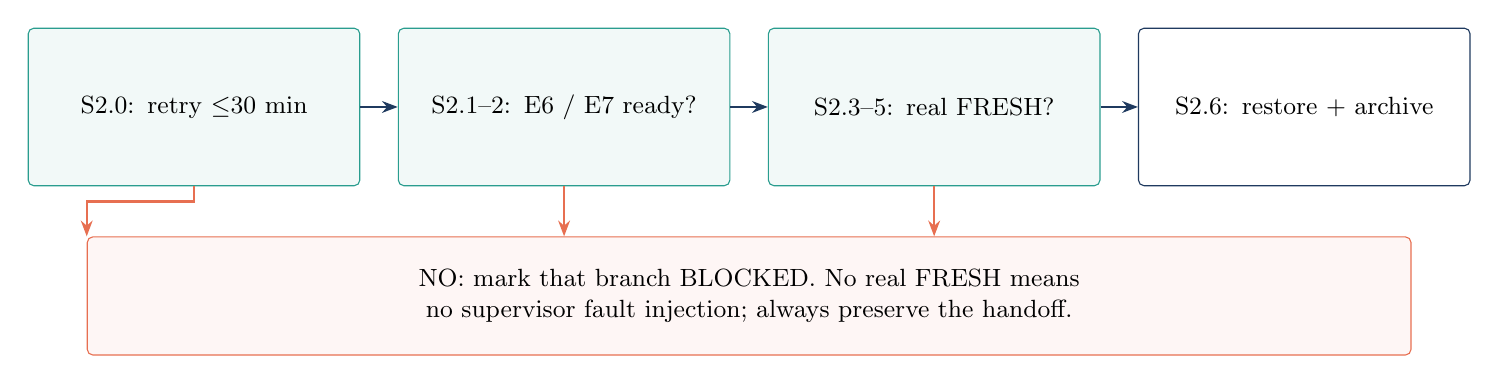
\begin{tikzpicture}\node[box,draw=teal,fill=teal!6,text width=40mm,minimum height=20mm] (m0) at (0.0,0) {S2.0: retry $\leq$30 min};\node[box,draw=teal,fill=teal!6,text width=40mm,minimum height=20mm] (m1) at (4.7,0) {S2.1–2: E6 / E7 ready?};\draw[flow] (m0.east)--(m1.west);\node[box,draw=teal,fill=teal!6,text width=40mm,minimum height=20mm] (m2) at (9.4,0) {S2.3–5: real FRESH?};\draw[flow] (m1.east)--(m2.west);\node[box,text width=40mm,minimum height=20mm] (m3) at (14.100000000000001,0) {S2.6: restore + archive};\draw[flow] (m2.east)--(m3.west);\node[box,draw=fault,fill=fault!6,text width=166mm,minimum height=15mm] (stop) at (7.05,-2.4) {NO: mark that branch BLOCKED. No real FRESH means no supervisor fault injection; always preserve the handoff.};\draw[faultflow] (m0.south)--(0,-1.2)-|(stop.north west);\draw[faultflow] (m1.south)--(m1.south|-stop.north);\draw[faultflow] (m2.south)--(m2.south|-stop.north);\end{tikzpicture}}{YES follows the top arrows; failed readiness follows the lower branch. Stop at 150 minutes.}\vfill\takeaway{Read the step card before its commands. Preserve failed and skipped work as evidence.}
\note{BRIEF2.md; matching timelines and step criteria. No operational command changed.}
\end{frame}
\begin{frame}{Session 2 timeline: 150 min maximum}
\evidence{ASSUMED wall-time budget}
\begin{tabular}{@{}L{57mm}L{123mm}@{}}\toprule
\textbf{Elapsed} & \textbf{Task / exit artifact}\\\midrule
0–30 min & S2.0: one corrected rerun per failed/marginal S1 branch.\\[6pt]
30–65 min & S2.1: E6 two-Pi edge run; selected sweep, not full campaign.\\[6pt]
65–95 min & S2.2: E7-C real-UART readiness / bounded trial.\\[6pt]
95–130 / 130–150 min & S2.3–6: CN/OS fault demo; verified archive and stop.\\[6pt]\bottomrule\end{tabular}\vfill\takeaway{If E7/supervisor preparation is missing, document BLOCKED; do not improvise firmware.}
\note{Study synthesis from base/main-v4-91p.tex, updated against base/main.tex. No new physical evidence; every gate remains OPEN.}
\end{frame}
\begin{frame}{S2.0 | Rerun only the earliest failed S1 condition}
\evidence{SOURCE-SUPPORTED procedure / execution OPEN}
\textbf{Goal / why:} Use the first 30 min to revisit the earliest failed Session-1 condition with one specific correction.\par\medskip\textbf{Physical setup:} Read handoff.md, rebind P0 to the new Session-2 RUN and DATA roots, and recheck power and identity. Renew N1 after a reboot or topology change.\par\medskip\textbf{What you see:} Each rerun has a fresh ID, the same original acceptance rule and a note naming the one cause changed. Old evidence remains untouched.
\note{Calibration plan, gate receipt rules and S1 handoff. S2 date is an explicit run-ID example. }
\end{frame}
\begin{frame}{S2.0 | Decision, recovery and files}
\evidence{SOURCE-SUPPORTED procedure / execution OPEN}
\textbf{PASS / FAIL:} A rerun passes only if it meets the original numeric and observable criteria. Stop retries at minute 30; unresolved work stays OPEN.\par\medskip\textbf{If FAIL:} Preserve the new failure and defer further WBR work. Continue independent CN tests only if their own power and physical prerequisites are healthy.\par\medskip\textbf{Take these files home:} Keep DATA/new-retry-ID, the matching RUN logs, fresh receipts and RUN/S2-rerun-ledger.md beside the Session-1 handoff.
\note{Calibration plan, gate receipt rules and S1 handoff. S2 date is an explicit run-ID example. }
\end{frame}
\begin{frame}[fragile]{S2.0 | Pi / control, fresh bindings (1/1)}
\evidence{SOURCE-SUPPORTED procedure / execution OPEN}
\begin{lstlisting}
export RUN="$HOME/wbr-evidence/study-S2-20261019"
export DATA="$HOME/wbr-takes/study-S2-20261019"
mkdir -p "$RUN" "$DATA"
vcgencmd get_throttled > "$RUN/power-before.txt"
lsusb -t > "$RUN/usb-before.txt"
# Repeat only the failed S1 step, with new output paths/IDs.
# Example ID=C2-ROS-retry01; same S1.5/S1.7 recipe.
# Reboot/topology change: renew N1; never reuse the old receipt.
\end{lstlisting}
\vfill\takeaway{Use the checks and failure branch on the preceding S2.0 step card.}
\note{Calibration plan, gate receipt rules and S1 handoff. S2 date is an explicit run-ID example.}
\end{frame}
\begin{frame}{S2.1 | CN/OS integration: E6 two-Pi edge offloading}
\evidence{SOURCE-SUPPORTED procedure / execution OPEN}
\textbf{Goal / why:} Run E6 on the two real Pis to distinguish client-clock network RTT from server-local queue and service time.\par\medskip\textbf{Physical setup:} Disconnect the camera. Use the 8 GB Pi B as edge server and the 4 GB Pi A as client, each with its own supply. Connect Ethernet and keep local consoles available.\par\medskip\textbf{What you see:} Wait for the server’s READY line before starting the client. The client writes frames.csv and meta.json; the server writes service-times.csv.
\note{CN hw/README.md, hw/\{edge\_server,sender,run\_e6,os\_inference\}.py; configs/E6hw.yaml; docs/HARDWARE.md (owner 16 Oct). \textasciitilde{}/CN is the explicit pre-lab deployment location on both Pis; do not assume it exists without P0. Address commands are source examples for unused 192.168.77.0/24 and require local console if Ethernet carries SSH. Do not mutate a management route blindly. E6 sweep declares synthetic 4 ms service; --queue latest is explicitly logged. No ONNX claim: optional ONNX needs actual model/runtime/hash, separate root and compatible config. Default runner includes separate preflight per run and validates route; 1-client E6 hardware is not equal to 2-client simulator.}
\end{frame}
\begin{frame}{S2.1 | Decision, recovery and files}
\evidence{SOURCE-SUPPORTED procedure / execution OPEN}
\textbf{PASS / FAIL:} The ASSUMED smoke check expects 200 terminal outcomes for 20 s at 10 fps, with no unidentified frame. Report actual loss/late replies and require clean power.\par\medskip\textbf{If FAIL:} Check power, route/interface, server/port, transport and queue/service in order. Retry once with a fresh output; never subtract unsynchronized absolute host times.\par\medskip\textbf{Take these files home:} Take home client results\_hw/E6/study-S2-* and server hw/results/study-S2-* with preflight, model/OS identities, commands and power readings.
\note{CN hw/README.md, hw/\{edge\_server,sender,run\_e6,os\_inference\}.py; configs/E6hw.yaml; docs/HARDWARE.md (owner 16 Oct). \textasciitilde{}/CN is the explicit pre-lab deployment location on both Pis; do not assume it exists without P0. Address commands are source examples for unused 192.168.77.0/24 and require local console if Ethernet carries SSH. Do not mutate a management route blindly. E6 sweep declares synthetic 4 ms service; --queue latest is explicitly logged. No ONNX claim: optional ONNX needs actual model/runtime/hash, separate root and compatible config. Default runner includes separate preflight per run and validates route; 1-client E6 hardware is not equal to 2-client simulator.}
\end{frame}
\begin{frame}[fragile]{S2.1 | 8 GB server B / \textasciitilde{}/CN prepared checkout (1/3)}
\evidence{SOURCE-SUPPORTED procedure / execution OPEN}
\begin{lstlisting}
cd ~/CN
sudo ip link set eth0 up
sudo ip address replace 192.168.77.2/24 dev eth0
sh hw/preflight.sh eth0 /tmp/e6-server-before.json
python3 hw/edge_server.py --host 192.168.77.2 --port 9000 \
  --transport udp --mode synthetic --sleep-ms 4 \
  --queue latest \
  --service-log hw/results/study-S2-udp/service-times.csv
\end{lstlisting}
\vfill\takeaway{Use the checks and failure branch on the preceding S2.1 step card.}
\note{CN hw/README.md, hw/\{edge\_server,sender,run\_e6,os\_inference\}.py; configs/E6hw.yaml; docs/HARDWARE.md (owner 16 Oct).}
\end{frame}
\begin{frame}[fragile]{S2.1 | 4 GB client A / local console, after READY (2/3)}
\evidence{SOURCE-SUPPORTED procedure / execution OPEN}
\begin{lstlisting}
cd ~/CN
sudo ip link set eth0 up
sudo ip address replace 192.168.77.1/24 dev eth0
ping -c 3 192.168.77.2
python3 hw/sender.py --host 192.168.77.2 --transport udp \
  --frame-bytes 30000 --fps 10 --duration 20 \
  --out-dir results_hw/E6/study-S2-smoke-udp-01
python3 hw/run_e6.py --link ethernet --transport udp \
  --dry-run
\end{lstlisting}
\vfill\takeaway{Use the checks and failure branch on the preceding S2.1 step card.}
\note{CN hw/README.md, hw/\{edge\_server,sender,run\_e6,os\_inference\}.py; configs/E6hw.yaml; docs/HARDWARE.md (owner 16 Oct).}
\end{frame}
\begin{frame}[fragile]{S2.1 | 4 GB client A / selected E6 pass (3/3)}
\evidence{SOURCE-SUPPORTED procedure / execution OPEN}
\begin{lstlisting}
# After reviewed smoke; 30 runs x20s, plus overhead.
python3 hw/run_e6.py --link ethernet --transport udp \
  --output-root results_hw/E6/study-S2-wired-udp-01
# Repeat TCP only after stopping/restarting server as TCP.
# Wi-Fi: existing AP; verify route dev wlan0 before any run.
# Full four-pass /120-run campaign is outside this session.
# Retain both Pi models, supplies, clocks and before/after flags.
\end{lstlisting}
\vfill\takeaway{Use the checks and failure branch on the preceding S2.1 step card.}
\note{CN hw/README.md, hw/\{edge\_server,sender,run\_e6,os\_inference\}.py; configs/E6hw.yaml; docs/HARDWARE.md (owner 16 Oct).}
\end{frame}
\begin{frame}{S2.1W | CN/OS integration: Wi-Fi / ONNX branches}
\evidence{SOURCE-SUPPORTED procedure / execution OPEN}
\textbf{Goal / why:} Keep optional Wi-Fi and ONNX comparisons tied to the transport and compute workload actually used.\par\medskip\textbf{Physical setup:} Use the existing access point and local consoles. Both endpoints must select the same transport. ONNX requires a prepared compatible model and runtime.\par\medskip\textbf{What you see:} The route to Pi B says dev wlan0. RTT uses the sender clock; queue and service durations use the server clock. ONNX failures remain visible.
\note{CN hw/README.md Wi-Fi and ONNX sections; hw/os\_inference.py fixed-image preprocessing. Network bytes are load, not decoded JPEG inference. Freeze transport, payload, fps, model/hash, threads and queue to compare. Remote absolute t\_rx/t\_start/t\_done stay empty; do not derive them from RTT. No hardware E6 result is established by writing this deck.}
\end{frame}
\begin{frame}{S2.1W | Decision, recovery and files}
\evidence{SOURCE-SUPPORTED procedure / execution OPEN}
\textbf{PASS / FAIL:} Require the intended route and retained outcomes for every generated frame. An absent model/runtime means ONNX is UNKNOWN; a synthetic run cannot qualify it.\par\medskip\textbf{If FAIL:} Stop the Wi-Fi branch if the route is wrong; do not reconfigure the AP in lab. If ONNX is unavailable, retain a clearly labeled synthetic result instead.\par\medskip\textbf{Take these files home:} Use fresh results\_hw/E6/study-S2-wifi-* or ONNX run roots. Keep the actual model hash, server service log and both Pi configurations.
\note{CN hw/README.md Wi-Fi and ONNX sections; hw/os\_inference.py fixed-image preprocessing. Network bytes are load, not decoded JPEG inference. Freeze transport, payload, fps, model/hash, threads and queue to compare. Remote absolute t\_rx/t\_start/t\_done stay empty; do not derive them from RTT. No hardware E6 result is established by writing this deck.}
\end{frame}
\begin{frame}[fragile]{S2.1W | 8 GB server B / existing Wi-Fi (1/3)}
\evidence{SOURCE-SUPPORTED procedure / execution OPEN}
\begin{lstlisting}
WIFI_B=$(ip -4 -o address show dev wlan0 scope global \
  | awk '{split($4,a,"/"); print a[1]; exit}')
python3 hw/edge_server.py --host "$WIFI_B" \
  --transport udp --mode synthetic --sleep-ms 4 \
  --service-log hw/results/study-S2-wifi/service-times.csv
\end{lstlisting}
\vfill\takeaway{Use the checks and failure branch on the preceding S2.1W step card.}
\note{CN hw/README.md Wi-Fi and ONNX sections; hw/os\_inference.py fixed-image preprocessing.}
\end{frame}
\begin{frame}[fragile]{S2.1W | 4 GB client A / use server printed IPv4 (2/3)}
\evidence{SOURCE-SUPPORTED procedure / execution OPEN}
\begin{lstlisting}
read -r -p 'Pi B Wi-Fi IPv4 address: ' WIFI_B
ip route get "$WIFI_B"
# Continue only if route is dev wlan0.
python3 hw/sender.py --host "$WIFI_B" --transport udp \
  --frame-bytes 30000 --fps 10 --duration 20 \
  --out-dir results_hw/E6/study-S2-wifi-udp-01
# Repeat as -02/-03 if time; TCP requires matching server.
# Optional ONNX service syntax (separate run/config):
# --mode onnx --model EXISTING_MODEL.onnx --threads 1
\end{lstlisting}
\vfill\takeaway{Use the checks and failure branch on the preceding S2.1W step card.}
\note{CN hw/README.md Wi-Fi and ONNX sections; hw/os\_inference.py fixed-image preprocessing.}
\end{frame}
\begin{frame}[fragile]{S2.1W | 8 GB server B / OPTIONAL prepared ONNX branch (3/3)}
\evidence{SOURCE-SUPPORTED procedure / execution OPEN}
\begin{lstlisting}
# UNVERIFIED installed model/runtime; use a separate run root.
cd ~/CN
test -s offline-bundle/mobilenetv2-12.onnx
sha256sum offline-bundle/mobilenetv2-12.onnx
python3 hw/edge_server.py --host 192.168.77.2 --port 9000 \
  --transport udp --mode onnx \
  --model offline-bundle/mobilenetv2-12.onnx --threads 1 \
  --queue latest \
  --service-log hw/results/study-S2-onnx/service-times.csv
# Client: S2.1 sender, new output name study-S2-onnx-01.
# Do not use unchanged synthetic-4ms E6 sweep config here.
\end{lstlisting}
\vfill\takeaway{Use the checks and failure branch on the preceding S2.1W step card.}
\note{CN hw/README.md Wi-Fi and ONNX sections; hw/os\_inference.py fixed-image preprocessing.}
\end{frame}
\begin{frame}{S2.2 | CN/OS integration: E7-C UART gateway trial}
\evidence{SOURCE-SUPPORTED procedure / execution OPEN}
\textbf{Goal / why:} Run E7 option C to add real STM32 UART ingress while measuring UART and network intervals separately.\par\medskip\textbf{Physical setup:} Use the owner-prepared E7 CubeMX image, gateway Pi A and edge Pi B. Cross the selected 3.3 V UART pins, join ground and confirm the port is not a console.\par\medskip\textbf{What you see:} CRC-checked image chunks assemble at the gateway and reach the edge. Each unique frame receives a terminal outcome with UART and network fields.
\note{CN docs/E7\_DESIGN.md option C, docs/CODEX\_TICKETS.md E7/E7d2/T18; e7/README.md and gateway.py. E7 image format is not WBR link bench or OS UART framing. Default firmware has fixed 1$\times$1 JPEG, no trained tiny-CNN. USART2 PA2/PA3 uses ST-LINK VCP; USART1 direct route PA9 TX$\to$Pi15 RX, PA10 RX$\leftarrow$Pi14 TX; qualify solder bridges and port. Start 115200 8N1; 921600/2M sustained hardware reliability UNTESTED. At least 100 transfers per size/baud and 3 network repetitions are full design qualification outside this short smoke trial. UART response-to-MCU egress is unimplemented. No cloud endpoint is selected; cloud branch deferred.}
\end{frame}
\begin{frame}{S2.2 | Decision, recovery and files}
\evidence{SOURCE-SUPPORTED procedure / execution OPEN}
\textbf{PASS / FAIL:} The design requires unique IDs, one terminal outcome per frame and no corrupt forwarding. Real baud reliability and MCU inference remain UNTESTED until measured.\par\medskip\textbf{If FAIL:} Check power, ground/pins, baud/console, CRC/chunks and server in order. A missing built image blocks this branch; no flash command may be guessed.\par\medskip\textbf{Take these files home:} Preserve results\_hw/E7/study-S2-edge-udp-01 with args.json, frames.csv and outcomes.jsonl, plus the actual firmware/config hashes.
\note{CN docs/E7\_DESIGN.md option C, docs/CODEX\_TICKETS.md E7/E7d2/T18; e7/README.md and gateway.py. E7 image format is not WBR link bench or OS UART framing. Default firmware has fixed 1$\times$1 JPEG, no trained tiny-CNN. USART2 PA2/PA3 uses ST-LINK VCP; USART1 direct route PA9 TX$\to$Pi15 RX, PA10 RX$\leftarrow$Pi14 TX; qualify solder bridges and port. Start 115200 8N1; 921600/2M sustained hardware reliability UNTESTED. At least 100 transfers per size/baud and 3 network repetitions are full design qualification outside this short smoke trial. UART response-to-MCU egress is unimplemented. No cloud endpoint is selected; cloud branch deferred.}
\end{frame}
\begin{frame}[fragile]{S2.2 | 4 GB gateway A / \textasciitilde{}/CN (1/1)}
\evidence{SOURCE-SUPPORTED procedure / execution OPEN}
\begin{lstlisting}
# UNVERIFIED hardware: owner's E7 firmware and real UART.
python3 e7/gateway/gateway.py --serial /dev/serial0 \
  --baud 115200 --host 192.168.77.2 --port 9000 \
  --transport udp --reply-format timed \
  --outDir results_hw/E7/study-S2-edge-udp-01
# Stop normally with Ctrl-C after the bounded fixture trial.
# Repeat TCP only with matching timed-reply server.
# No --net-status-ms here until a compatible supervisor exists.
\end{lstlisting}
\vfill\takeaway{Use the checks and failure branch on the preceding S2.2 step card.}
\note{CN docs/E7\_DESIGN.md option C, docs/CODEX\_TICKETS.md E7/E7d2/T18; e7/README.md and gateway.py.}
\end{frame}
\begin{frame}{S2.3 | CN/OS integration: supervisor readiness}
\evidence{SOURCE-SUPPORTED procedure / execution OPEN}
\textbf{Goal / why:} Establish real-UART FRESH before fault injection, so a later state change has a verified healthy starting point.\par\medskip\textbf{Physical setup:} Use the compatible OS v3 board image, one hea\_bridge UART writer and a prepared CN-result IPC producer. Replace the E7 image/path; do not run both UART writers.\par\medskip\textbf{What you see:} Accepted local HEARTBEAT, INFERENCE and NET\_STATUS make MCU\_STATUS report FRESH=1. Save the real MCU state and clock telemetry.
\note{OS-wt-cn docs/CN\_INTEGRATION.md and protocol/PROTOCOL.md; CN e7/gateway/NET\_STATUS.md. This is a pre-lab integration dependency, not a fabricated executable. Original requested OS protocol v1 names INIT/FRESH/HOLD/FAILSAFE but NET\_STATUS is a later v3 extension in OS-wt-cn. Updated full board image status is UNKNOWN there; only portable sources cross-compiled and host tests passed. Existing E7 gateway --net-status-ms 20 can emit v3 HB/status with one sequence, but sends no INFERENCE or MCU clock map and alone cannot satisfy supervisor local readiness. IPC clock stamps must be explicitly mapped to gateway RAW; remote host times are invalid.}
\end{frame}
\begin{frame}{S2.3 | Decision, recovery and files}
\evidence{SOURCE-SUPPORTED procedure / execution OPEN}
\textbf{PASS / FAIL:} Continue only after state 1 is actually observed and recorded. Sources report host/PTY tests only; the real UART path is still UNTESTED.\par\medskip\textbf{If FAIL:} Stop if the image, producer or FRESH state is missing. E7 telemetry alone sends no INFERENCE and cannot satisfy the supervisor’s local readiness checks.\par\medskip\textbf{Take these files home:} Retain bridge.csv, inf\_rx.csv, state\_events.csv and readiness notes, together with the exact OS firmware and configuration hashes.
\note{OS-wt-cn docs/CN\_INTEGRATION.md and protocol/PROTOCOL.md; CN e7/gateway/NET\_STATUS.md. This is a pre-lab integration dependency, not a fabricated executable. Original requested OS protocol v1 names INIT/FRESH/HOLD/FAILSAFE but NET\_STATUS is a later v3 extension in OS-wt-cn. Updated full board image status is UNKNOWN there; only portable sources cross-compiled and host tests passed. Existing E7 gateway --net-status-ms 20 can emit v3 HB/status with one sequence, but sends no INFERENCE or MCU clock map and alone cannot satisfy supervisor local readiness. IPC clock stamps must be explicitly mapped to gateway RAW; remote host times are invalid.}
\end{frame}
\begin{frame}[fragile]{S2.3 | Gateway Pi / prepared OS checkout (1/1)}
\evidence{SOURCE-SUPPORTED procedure / execution OPEN}
\begin{lstlisting}
# UNVERIFIED: deployed image, UART and CN-result IPC producer.
# Source interface exists; this hardware recipe is not validated.
linux/build/hea_bridge --socket /tmp/cn-results.sock \
  --serial /dev/ttyAMA0 --baud 921600 \
  --heartbeat-ms 20 --net-status-ms 20 --policy latest \
  --csv bridge.csv
# Do NOT run E7 gateway as another writer to the same UART.
# CN producer must provide accepted <IQQBBI IPC records.
# No verified producer/flash command is supplied: STOP if absent.
\end{lstlisting}
\vfill\takeaway{Use the checks and failure branch on the preceding S2.3 step card.}
\note{OS-wt-cn docs/CN\_INTEGRATION.md and protocol/PROTOCOL.md; CN e7/gateway/NET\_STATUS.md.}
\end{frame}
\begin{frame}{S2.4 | CN/OS integration: Wi-Fi loss while heartbeat lives}
\evidence{SOURCE-SUPPORTED procedure / execution OPEN}
\textbf{Goal / why:} Interrupt network results while keeping local heartbeat alive, so the MCU can demonstrate stale-result HOLD followed by latched FAILSAFE.\par\medskip\textbf{Physical setup:} Start from recorded FRESH on a motor-free bench. Keep local heartbeat at 20 ms and use the transmitting result peer’s wlan0, with local console recovery available.\par\medskip\textbf{What you see:} The source defaults predict HOLD at result/network age $\geq$200 ms and FAILSAFE $\geq$500 ms. These are provisional configuration values, not measured WBR safety bounds.
\note{OS-wt-cn scripts/netem\_inject.sh; docs/CN\_INTEGRATION.md network age/silence transitions; CN synergy part 6. Loss injection is outbound root qdisc; clear deletes instead of restoring previous custom qdisc. Do not apply on an interface with a valued existing root policy; prepare isolated link beforehand. On server B, lost replies stop accepted results at gateway; HB continues locally. This is controlled Wi-Fi result-delivery loss, not a proof of radio disassociation. An actual AP outage can be added manually only after recording network path; expected state semantics stay the same. Loss telemetry counts result identities, not raw Wi-Fi packet loss.}
\end{frame}
\begin{frame}{S2.4 | Decision, recovery and files}
\evidence{SOURCE-SUPPORTED procedure / execution OPEN}
\textbf{PASS / FAIL:} Require recorded state order 1$\to$2$\to$3 with age/silence reasons and no unexplained missing events. A stopped local heartbeat tests a different failure path.\par\medskip\textbf{If FAIL:} Restore the result path and keep the failed trace. If heartbeat also stopped, label that attempt accordingly; do not change timeouts to obtain the desired sequence.\par\medskip\textbf{Take these files home:} Keep bridge.csv, state\_events.csv, fault-on/off observations and the gateway/server interface and config records. Measure transitions on a supported clock.
\note{OS-wt-cn scripts/netem\_inject.sh; docs/CN\_INTEGRATION.md network age/silence transitions; CN synergy part 6. Loss injection is outbound root qdisc; clear deletes instead of restoring previous custom qdisc. Do not apply on an interface with a valued existing root policy; prepare isolated link beforehand. On server B, lost replies stop accepted results at gateway; HB continues locally. This is controlled Wi-Fi result-delivery loss, not a proof of radio disassociation. An actual AP outage can be added manually only after recording network path; expected state semantics stay the same. Loss telemetry counts result identities, not raw Wi-Fi packet loss.}
\end{frame}
\begin{frame}[fragile]{S2.4 | Wi-Fi transmitting peer / prepared OS scripts (1/1)}
\evidence{SOURCE-SUPPORTED procedure / execution OPEN}
\begin{lstlisting}
# UNVERIFIED real Wi-Fi/UART integration; source CLI verified.
# Affect outgoing results on edge server B, not management SSH.
scripts/netem_inject.sh --dry-run apply wlan0 --loss 100
# After owner checks the printed direction and local console:
scripts/netem_inject.sh apply wlan0 --loss 100
# Leave >500ms while gateway HEARTBEAT stays alive.
# Observe and save MCU states, then restore the path:
scripts/netem_inject.sh clear wlan0
\end{lstlisting}
\vfill\takeaway{Use the checks and failure branch on the preceding S2.4 step card.}
\note{OS-wt-cn scripts/netem\_inject.sh; docs/CN\_INTEGRATION.md network age/silence transitions; CN synergy part 6.}
\end{frame}
\begin{frame}{S2.5 | CN/OS integration: recover and test heartbeat loss}
\evidence{SOURCE-SUPPORTED procedure / execution OPEN}
\textbf{Goal / why:} Demonstrate recovery from latched FAILSAFE, then test heartbeat loss separately so the two mechanisms remain understandable.\par\medskip\textbf{Physical setup:} Restore the network while FAILSAFE is latched. On the motor-free bench, the owner resets the board; re-establish accepted heartbeat, inference and network status.\par\medskip\textbf{What you see:} After reset, expect INIT$\to$FRESH. A short HOLD-only interruption may recover automatically; stopping heartbeat instead predicts FAILSAFE near 100 ms.
\note{OS protocol v3 and docs/CN\_INTEGRATION.md explicit latched/rearm/board-reset policy. Network age includes reported age + local MCU silence + provisional transit allowance. Thresholds are configuration, not measured physical response guarantees. Measure MCU state-change time on MCU clock or validated mapping; shell/netem command duration is not wire fault onset. There is no remote rearm wire command. Board reset demonstrates this port’s recovery, not uninterrupted WBR balancing. Real robot must retain independent control by architecture; physical N7 remains OPEN.}
\end{frame}
\begin{frame}{S2.5 | Decision, recovery and files}
\evidence{SOURCE-SUPPORTED procedure / execution OPEN}
\textbf{PASS / FAIL:} Require FAILSAFE to remain latched on resumed packets alone. Reset and new readiness must precede FRESH. The 100 ms default is provisional, not a guaranteed physical response.\par\medskip\textbf{If FAIL:} Stop on an unexpected state and save raw protocol/state traces. A missing hardware result leaves robot control independence unproven; do not infer balancing from this bench.\par\medskip\textbf{Take these files home:} Preserve separate reset/recovery and heartbeat-loss traces, with fault/reset notes and exact thresholds. A bounded short-fault fixture is still UNVERIFIED.
\note{OS protocol v3 and docs/CN\_INTEGRATION.md explicit latched/rearm/board-reset policy. Network age includes reported age + local MCU silence + provisional transit allowance. Thresholds are configuration, not measured physical response guarantees. Measure MCU state-change time on MCU clock or validated mapping; shell/netem command duration is not wire fault onset. There is no remote rearm wire command. Board reset demonstrates this port’s recovery, not uninterrupted WBR balancing. Real robot must retain independent control by architecture; physical N7 remains OPEN.}
\end{frame}
\begin{frame}[fragile]{S2.5 | Gateway / manual controlled fault sequence (1/1)}
\evidence{SOURCE-SUPPORTED procedure / execution OPEN}
\begin{lstlisting}
# Restore Wi-Fi result path and preserve prior trace first.
# Owner presses board RESET after latched FAILSAFE.
# Verify fresh HB + INFERENCE + NET_STATUS -> INIT then FRESH.
# For HB-loss case: Ctrl-C the sole hea_bridge process.
# Expected provisional HB timeout: 100ms -> latched FAILSAFE.
# Resume bridge; packets alone do not clear the latch.
# Owner resets board, re-establishes FRESH; save a new trace.
# HOLD-only recovery needs measured <500ms result interruption.
# UNVERIFIED: bounded real-network short fault timing fixture.
\end{lstlisting}
\vfill\takeaway{Use the checks and failure branch on the preceding S2.5 step card.}
\note{OS protocol v3 and docs/CN\_INTEGRATION.md explicit latched/rearm/board-reset policy.}
\end{frame}
\begin{frame}{S2.6 | CN/OS integration: archive and interpret honestly}
\evidence{SOURCE-SUPPORTED procedure / execution OPEN}
\textbf{Goal / why:} Finish within 150 min with complete node/MCU evidence and an honest account of what was not tested.\par\medskip\textbf{Physical setup:} Stop jobs normally, clear the injected qdisc, and sample power on each Pi. Keep the Mac reachable while both node archives are copied.\par\medskip\textbf{What you see:} The cleared qdisc is checked explicitly. The archive contains client outcomes, server service logs, UART states, configs, identities and verified file hashes.
\note{CN hw/README.md, E7 retained timing contract; OS CN integration telemetry; WBR source handoff policy. }
\end{frame}
\begin{frame}{S2.6 | Decision, recovery and files}
\evidence{SOURCE-SUPPORTED procedure / execution OPEN}
\textbf{PASS / FAIL:} Require one recorded outcome per generated frame, valid clock boundaries and matching copies. Missing telemetry stays UNKNOWN and no hardware gate is promoted by this archive.\par\medskip\textbf{If FAIL:} Keep each node’s originals after a failed copy. Retry transfer once; do not delete files until the finalized manifests verify on the Mac.\par\medskip\textbf{Take these files home:} Take home study-S2-20261019/\{wbr,cn-client,cn-server,os\} and summary.md, including rerun evidence, fault/recovery traces and unresolved prerequisites.
\note{CN hw/README.md, E7 retained timing contract; OS CN integration telemetry; WBR source handoff policy. }
\end{frame}
\begin{frame}[fragile]{S2.6 | Each Pi / control (1/2)}
\evidence{SOURCE-SUPPORTED procedure / execution OPEN}
\begin{lstlisting}
vcgencmd get_throttled
vcgencmd pmic_read_adc EXT5V_V
# Save the raw values in that node's run directory.
# On edge peer if injection was used:
scripts/netem_inject.sh status wlan0
# Verify cleared qdisc; do not infer it from restored replies.
# Copy both CN results roots and OS CSVs to Mac; hash finalized files.
# Owner shuts down only after the archive verification.
\end{lstlisting}
\vfill\takeaway{Use the checks and failure branch on the preceding S2.6 step card.}
\note{CN hw/README.md, E7 retained timing contract; OS CN integration telemetry; WBR source handoff policy.}
\end{frame}
\begin{frame}[fragile]{S2.6 | Mac / both-node CN archive, then hash review (2/2)}
\evidence{SOURCE-SUPPORTED procedure / execution OPEN}
\begin{lstlisting}
export ARCH="$HOME/Desktop/Research/wbr-data/study-S2-20261019"
mkdir -p "$ARCH/cn-client" "$ARCH/cn-server" "$ARCH/os"
# UNVERIFIED deployment SSH targets/routes: bind from lab inventory.
read -r -p 'Client SSH user@host: ' CN_CLIENT_SSH
read -r -p 'Edge SSH user@host: ' CN_EDGE_SSH
rsync -a --checksum "$CN_CLIENT_SSH:CN/results_hw/" \
  "$ARCH/cn-client/"
rsync -a --checksum "$CN_EDGE_SSH:CN/hw/results/" \
  "$ARCH/cn-server/"
# OS trace dir is a pre-lab binding, not a guessed path.
# Copy bridge/inf_rx/state_events CSVs plus firmware/config hashes.
# Verify per-node finalized SHA256 manifests as in S1.5F.
\end{lstlisting}
\vfill\takeaway{Use the checks and failure branch on the preceding S2.6 step card.}
\note{CN hw/README.md, E7 retained timing contract; OS CN integration telemetry; WBR source handoff policy.}
\end{frame}
\begin{frame}{Session 2: what you take home — runs and traces}
\evidence{SOURCE-SUPPORTED inventory / hardware tests conditional}
\begin{tabular}{@{}L{94mm}L{86mm}@{}}\toprule
\textbf{Bag or file family} & \textbf{Home consumer}\\\midrule
WBR retry bags, native takes and fresh receipts & Same H0–H6 path as the corresponding S1 take.\\[6pt]
Both Pi E6 outcomes/meta/service/preflight logs & H0 archive check; H7 clock/coverage discipline only.\\[6pt]
E7 args/frames/outcomes + firmware identity & H0 archive check; separate CN timing analysis.\\[6pt]
OS bridge/inf\_rx/state events + faults/resets & H0 archive check; separate supervisor transition review.\\[6pt]\bottomrule\end{tabular}\vfill\takeaway{CN/OS CSVs are not trajectories and must not be fed to H7 ATE/RPE.}
\note{Study synthesis from base/main-v4-91p.tex, updated against base/main.tex. No new physical evidence; every gate remains OPEN.}
\end{frame}
\begin{frame}{Session 2: what you take home — context and decisions}
\evidence{SOURCE-SUPPORTED inventory / no new gate evidence}
\begin{tabular}{@{}L{94mm}L{86mm}@{}}\toprule
\textbf{Bag or file family} & \textbf{Home consumer}\\\midrule
Power before/after, qdisc status, node configs & H0 preservation; join with separate CN timing review.\\[6pt]
Model/binary/firmware hashes and exact commands & H0 integrity; H6 only for an actual WBR replay.\\[6pt]
RUN/S2-rerun-ledger, summary and SHA256SUMS & H0 decides usable inputs; H1–H7 skip absent branches.\\[6pt]
Independent route/reference, only if acquired & H7 metrics if compatible; otherwise report proxies.\\[6pt]\bottomrule\end{tabular}\vfill\takeaway{H1–H5 consume sensor data, not E6/E7 logs. Keep full hardware campaigns OPEN.}
\note{Study synthesis from base/main-v4-91p.tex, updated against base/main.tex. No new physical evidence; every gate remains OPEN.}
\end{frame}
\begin{frame}{At home: analyze immutable inputs}
\evidence{SOURCE-SUPPORTED offline workflow}
\deckitems{\item Begin with copied hashes, bag metadata, raw counts/timestamps and config identities.\item Then validate conversion, fit calibration/noise and replay the same data repeatedly.\item Only independent ground truth permits ATE/RPE; room routes provide proxies.}
\vfill\takeaway{Keep acquisition failures visible through every derivative.}
\note{Study synthesis from base/main-v4-91p.tex, updated against base/main.tex. No new physical evidence; every gate remains OPEN.}
\end{frame}
\begin{frame}{H0 | Home: bag metadata, replay and timestamps}
\evidence{SOURCE-SUPPORTED procedure / execution OPEN}
\textbf{Goal / why:} Check recording completeness before analysis; a bag that opens can still be missing data or context.\par\medskip\textbf{Physical setup:} Use finalized copied bags and sourced Jazzy at home. Stop live camera publishers and replay in the separate localhost domain.\par\medskip\textbf{What you see:} Bag information lists topics, types and counts. The audit must also examine source headers, clock domains, complete-window gaps and replay contents.
\note{n3\_bag.py play flags and strict replay contract; current calibration plan raw timing checks. Use both N/requested-window and (N−1)/(last−first) surviving-span rates; inspect boundaries, dt histograms, domains, sequence gaps and original metadata. ros2 topic hz is supplemental and does not prove zero loss. ROS$\to$SDK-audit conversion is absent; no invented check script. Record source header separately from rosbag storage time.}
\end{frame}
\begin{frame}{H0 | Decision, recovery and files}
\evidence{SOURCE-SUPPORTED procedure / execution OPEN}
\textbf{PASS / FAIL:} The ASSUMED review permits no unexplained loss/reversal and requires complete context plus replay count/header/pixel agreement. Bag-info alone cannot pass it.\par\medskip\textbf{If FAIL:} Resolve hashes/copy first, then context/QoS and original timestamp metadata. Do not sort, interpolate or fill damaged data to make the report pass.\par\medskip\textbf{Take these files home:} Keep derived bag-info, timing/count reports and replay logs beside the input hash manifest. Preserve all original bags unchanged.
\note{n3\_bag.py play flags and strict replay contract; current calibration plan raw timing checks. Use both N/requested-window and (N−1)/(last−first) surviving-span rates; inspect boundaries, dt histograms, domains, sequence gaps and original metadata. ros2 topic hz is supplemental and does not prove zero loss. ROS$\to$SDK-audit conversion is absent; no invented check script. Record source header separately from rosbag storage time.}
\end{frame}
\begin{frame}[fragile]{H0 | Home Linux / sourced Jazzy (1/1)}
\evidence{SOURCE-SUPPORTED procedure / execution OPEN}
\begin{lstlisting}
export BAG="$HOME/wbr-takes/study-S1-20261018/S-ROS-01/ros"
ros2 bag info "$BAG"
# Stop live wrapper first; use isolated localhost replay domain.
export ROS_DOMAIN_ID=43 ROS_LOCALHOST_ONLY=1
ros2 bag play "$BAG" --rate 1.0 --delay 3 \
  --qos-profile-overrides-path "$STUDY/lab-config/qos.yaml"
# In another domain-43 terminal: observe source headers/counts.
# UNVERIFIED: extended stereo/metadata bag audit interface.
# n3_bag.py accepts only its reviewed N3 receipt/topic contract.
\end{lstlisting}
\vfill\takeaway{Use the checks and failure branch on the preceding H0 step card.}
\note{n3\_bag.py play flags and strict replay contract; current calibration plan raw timing checks.}
\end{frame}
\begin{frame}{H1 | Home: native SDK bag audit and EuRoC export}
\evidence{SOURCE-SUPPORTED procedure / execution OPEN}
\textbf{Goal / why:} Identify and audit the native SDK schema before exporting EuRoC input, because a .db3 extension does not define its contents.\par\medskip\textbf{Physical setup:} On the Mac’s canonical WBR checkout, select an actual finalized native take and a fresh derived output root. No camera is needed.\par\medskip\textbf{What you see:} Inspection and audit produce schema/timing reports. Export creates lossless grayscale PNGs, raw gyro/accel, the combined grid, manifest and times\_ns.txt.
\note{tools/take\_tools/README.md and take\_tools.py; older experiments/2026-10-14-db3-to-euroc/db3\_to\_euroc.py inspected but not selected. Use take\_tools.py, not the older converter: it preserves Decimal SDK milliseconds$\to$integer ns, independent raw streams, pixel hashes, interpolation exclusions and strict times-file interior. The older db3\_to\_euroc.py uses different fixed assumptions; do not mix its CLI/schema. export-euroc expects native /device\_0/... metadata, not /camera/camera/... ordinary ROS bags. Take format is detected from magic, not extension. Native domain SYSTEM\_TIME is excluded by calibration policy even if a structural tool would accept it.}
\end{frame}
\begin{frame}{H1 | Decision, recovery and files}
\evidence{SOURCE-SUPPORTED procedure / execution OPEN}
\textbf{PASS / FAIL:} Require an allowed common source domain, valid order, no rejected gaps and nonempty image times strictly inside combined IMU coverage.\par\medskip\textbf{If FAIL:} Stop on unsupported schema, ROS1 magic or invalid timing. Do not rename the input or use a diagnostic override to claim qualification.\par\medskip\textbf{Take these files home:} Keep DERIVED/C1-native-euroc in full, plus the audit JSON/Markdown. Its manifest links pixels, timestamps and converter identity to the raw hash.
\note{tools/take\_tools/README.md and take\_tools.py; older experiments/2026-10-14-db3-to-euroc/db3\_to\_euroc.py inspected but not selected. Use take\_tools.py, not the older converter: it preserves Decimal SDK milliseconds$\to$integer ns, independent raw streams, pixel hashes, interpolation exclusions and strict times-file interior. The older db3\_to\_euroc.py uses different fixed assumptions; do not mix its CLI/schema. export-euroc expects native /device\_0/... metadata, not /camera/camera/... ordinary ROS bags. Take format is detected from magic, not extension. Native domain SYSTEM\_TIME is excluded by calibration policy even if a structural tool would accept it.}
\end{frame}
\begin{frame}[fragile]{H1 | Mac / canonical WBR checkout (1/1)}
\evidence{SOURCE-SUPPORTED procedure / execution OPEN}
\begin{lstlisting}
export ARCH="$HOME/Desktop/Research/wbr-data/study-S1-20261018"
export NATIVE="$ARCH/native/C1-NATIVE-01/take"
export DERIVED="$HOME/Desktop/Research/wbr-data/derived-study"
python3 tools/take_tools/take_tools.py inspect \
  "$NATIVE/stereo_imu.db3"
python3 tools/take_tools/take_tools.py audit \
  "$NATIVE/stereo_imu.db3" --json /tmp/C1-audit.json \
  --markdown /tmp/C1-audit.md
python3 tools/take_tools/take_tools.py export-euroc \
  "$NATIVE/stereo_imu.db3" "$DERIVED/C1-native-euroc"
\end{lstlisting}
\vfill\takeaway{Use the checks and failure branch on the preceding H1 step card.}
\note{tools/take\_tools/README.md and take\_tools.py; older experiments/2026-10-14-db3-to-euroc/db3\_to\_euroc.py inspected but not selected.}
\end{frame}
\begin{frame}{H2 | Home: native replica $\to$ derived ROS companion}
\evidence{SOURCE-SUPPORTED procedure / execution OPEN}
\textbf{Goal / why:} Test whether a native take can produce a faithful ROS companion through file playback, without two programs opening the camera.\par\medskip\textbf{Physical setup:} Physically unplug the camera. Prepare the explicit ROS recorder before starting wrapper file playback from the finalized native SDK file.\par\medskip\textbf{What you see:} The source exposes rosbag\_filename, but this target db3’s startup and stamp preservation have not been validated. A derived ROS bag is the expected candidate output.
\note{Local realsense-ros realsense\_node\_factory.cpp load\_device and rs\_launch.py rosbag\_filename/rosbag\_loop; live\_record\_db3\_play test source. A native SDK .db3 is a recording format, not an ordinary wrapper topic bag. Wrapper playback may remap stamps or begin before discovery; source support does not prove exact conversion. A native replica is not scheduled until this requirement is validated. The mandated ROS companions for native N2/vendor CSV and native Allan CSV remain absent. This is a material input-tool gap recorded in REVIEW\_LOG.md.}
\end{frame}
\begin{frame}{H2 | Decision, recovery and files}
\evidence{SOURCE-SUPPORTED procedure / execution OPEN}
\textbf{PASS / FAIL:} This route remains UNVERIFIED until complete counts, first/last IDs, original stamps/domains and pixels match exactly. A readable derived bag is insufficient.\par\medskip\textbf{If FAIL:} Keep the native file and mark conversion BLOCKED after any missing boundary, rewritten stamp or unsupported schema. Do not schedule native replicas until this gap is resolved.\par\medskip\textbf{Take these files home:} Retain derived/C1-native-ros and a conversion receipt linking its input hash and full-window comparisons. Failed candidate conversions remain evidence.
\note{Local realsense-ros realsense\_node\_factory.cpp load\_device and rs\_launch.py rosbag\_filename/rosbag\_loop; live\_record\_db3\_play test source. A native SDK .db3 is a recording format, not an ordinary wrapper topic bag. Wrapper playback may remap stamps or begin before discovery; source support does not prove exact conversion. A native replica is not scheduled until this requirement is validated. The mandated ROS companions for native N2/vendor CSV and native Allan CSV remain absent. This is a material input-tool gap recorded in REVIEW\_LOG.md.}
\end{frame}
\begin{frame}[fragile]{H2 | Home ROS / file publisher, no live camera (1/1)}
\evidence{SOURCE-SUPPORTED procedure / execution OPEN}
\begin{lstlisting}
# UNVERIFIED: db3 load and lossless full-window behavior.
# Start ros2 bag record with the S1.5 explicit topic list first.
ros2 launch realsense2_camera rs_launch.py \
  config_file:="$STUDY/lab-config/ros-stereo.yaml" \
  rosbag_filename:="$NATIVE/stereo_imu.db3" rosbag_loop:=false
# No tested pause/start handshake exists in this recipe.
# Never claim this derived replay is a second live measurement.
# Native A CSV has no rosbag_filename route: see H3.
\end{lstlisting}
\vfill\takeaway{Use the checks and failure branch on the preceding H2 step card.}
\note{Local realsense-ros realsense\_node\_factory.cpp load\_device and rs\_launch.py rosbag\_filename/rosbag\_loop; live\_record\_db3\_play test source.}
\end{frame}
\begin{frame}{H3 | Home: conversion boundary and preparation gaps}
\evidence{SOURCE-SUPPORTED procedure / execution OPEN}
\textbf{Goal / why:} Keep schema boundaries explicit before fitting: native SDK bags, wrapper ROS bags and native IMU CSV are different inputs.\par\medskip\textbf{Physical setup:} Use the source-supported native S/C converter only on its expected take directory. Have the fixed Foundation path and prepared Kalibr image verified.\par\medskip\textbf{What you see:} The native helper creates ROS1 take.bag. Ordinary ROS S/C-to-Kalibr and raw A extraction still lack reviewed adapters; the commands mark those gaps UNVERIFIED.
\note{calibration/lab/mac/take\_to\_kalibr\_bag.sh and README.md; tools/take\_tools native schema. The Kalibr helper calls an exact fixed Foundation tool path /Users/quockaiser/Desktop/Research/wbr-sw-foundation/tools/take\_tools/take\_tools.py, not automatically this worktree copy. Verify its source hash and prepared Docker image before use. common.sh hard-codes FOUNDATION and IMAGE; there is no environment override. Verify the fixed paths/image; never invent LAB\_FOUNDATION. ROS1 output topics are /cam0/image\_raw /cam1/image\_raw /imu0. Do not pass --diagnostic for accepted calibration.}
\end{frame}
\begin{frame}{H3 | Decision, recovery and files}
\evidence{SOURCE-SUPPORTED procedure / execution OPEN}
\textbf{PASS / FAIL:} Require matching counts/pixels/SI units and source-stamp error $\leq$1 $\mu$s after conversion. An absent extractor blocks that analysis branch.\par\medskip\textbf{If FAIL:} Stop fitting and prepare the missing conversion at home. Never invent a program or substitute recorder write time for sensor source time.\par\medskip\textbf{Take these files home:} Keep the native Kalibr output, input/output hashes and count/stamp/pixel receipt. Preserve every rejected derivative separately.
\note{calibration/lab/mac/take\_to\_kalibr\_bag.sh and README.md; tools/take\_tools native schema. The Kalibr helper calls an exact fixed Foundation tool path /Users/quockaiser/Desktop/Research/wbr-sw-foundation/tools/take\_tools/take\_tools.py, not automatically this worktree copy. Verify its source hash and prepared Docker image before use. common.sh hard-codes FOUNDATION and IMAGE; there is no environment override. Verify the fixed paths/image; never invent LAB\_FOUNDATION. ROS1 output topics are /cam0/image\_raw /cam1/image\_raw /imu0. Do not pass --diagnostic for accepted calibration.}
\end{frame}
\begin{frame}[fragile]{H3 | Mac / native S/C only (1/1)}
\evidence{SOURCE-SUPPORTED procedure / execution OPEN}
\begin{lstlisting}
cd ~/Desktop/Research/wbr-perception-phase1-runtime
bash calibration/lab/mac/take_to_kalibr_bag.sh \
  "$NATIVE" "$DERIVED/C1-native-kalibr"
# Repeat independently for C2, C3 and S native takes.
# UNVERIFIED: wrapper ROS bag -> Kalibr source-stamp exporter.
# UNVERIFIED: ROS raw IMU -> Allan CSV extraction.
# UNVERIFIED: native Allan / native N2 -> ROS companion.
# No executable for those absent interfaces is claimed.
\end{lstlisting}
\vfill\takeaway{Use the checks and failure branch on the preceding H3 step card.}
\note{calibration/lab/mac/take\_to\_kalibr\_bag.sh and README.md; tools/take\_tools native schema.}
\end{frame}
\begin{frame}{H4 | Home: Kalibr C fits and stereo validation}
\evidence{SOURCE-SUPPORTED procedure / execution OPEN}
\textbf{Goal / why:} Compare residuals and independent repeats before selecting a spatial/time candidate for later review.\par\medskip\textbf{Physical setup:} Use audited native-to-ROS1 bags, the physically measured target YAML and the prepared Intel-Mac Kalibr image. Keep factory operating settings unchanged.\par\medskip\textbf{What you see:} Each C fit produces a report, results and camera chain. The S stereo check produces its own report; ORB YAML files remain candidates.
\note{calibration/lab/mac/\{run\_kalibr\_camimu,run\_kalibr\_stereo\_check\}.sh and summarize\_kalibr.py. Cam-IMU uses --cams plural, fixed factory chain, calibrated IMU model and default temporal estimation. Do not pass --no-time-calibration. Report radial RMS from pixel mean/std, not normalized residual or mean alone. Check all axes/residual structure/failed detections, proper orthonormal R, det≈+1, CAD $\leq$5mm/2$^\circ$ as comparison, not forced truth. Candidate converter emits PinHole; current operating model Rectified. Review rectification before deployment and apply time shift once via a separately reviewed hook; no ORB YAML time-offset field exists.}
\end{frame}
\begin{frame}{H4 | Decision, recovery and files}
\evidence{SOURCE-SUPPORTED procedure / execution OPEN}
\textbf{PASS / FAIL:} ASSUMED review: radial RMS $\leq$0.5 px, C1–C3 spread $\leq$3 mm/1$^\circ$ and time-shift spread $\leq$1 ms. S validation baseline should differ by $\leq$1 mm.\par\medskip\textbf{If FAIL:} Inspect timing, target/light, motion, transform direction and noise in order. Do not replace factory settings based on an attractive single fit.\par\medskip\textbf{Take these files home:} Keep DERIVED/C1-imucam through C3 and S-stereo with PDFs, logs and candidate files. Record noise source and every failed detection/residual pattern.
\note{calibration/lab/mac/\{run\_kalibr\_camimu,run\_kalibr\_stereo\_check\}.sh and summarize\_kalibr.py. Cam-IMU uses --cams plural, fixed factory chain, calibrated IMU model and default temporal estimation. Do not pass --no-time-calibration. Report radial RMS from pixel mean/std, not normalized residual or mean alone. Check all axes/residual structure/failed detections, proper orthonormal R, det≈+1, CAD $\leq$5mm/2$^\circ$ as comparison, not forced truth. Candidate converter emits PinHole; current operating model Rectified. Review rectification before deployment and apply time shift once via a separately reviewed hook; no ORB YAML time-offset field exists.}
\end{frame}
\begin{frame}[fragile]{H4 | Mac / canonical WBR checkout (1/1)}
\evidence{SOURCE-SUPPORTED procedure / execution OPEN}
\begin{lstlisting}
export TARGET="$HOME/Desktop/Research/wbr-data/measured-target.yaml"
bash calibration/lab/mac/run_kalibr_camimu.sh \
  "$DERIVED/C1-native-kalibr/take.bag" "$TARGET" \
  "$DERIVED/C1-imucam"
# Repeat with C2/C3 input/output names, no overwrites.
# Optional fourth arg is a supported measured IMU noise YAML.
bash calibration/lab/mac/run_kalibr_stereo_check.sh \
  "$DERIVED/S-native-kalibr/take.bag" "$TARGET" \
  "$DERIVED/S-stereo"
\end{lstlisting}
\vfill\takeaway{Use the checks and failure branch on the preceding H4 step card.}
\note{calibration/lab/mac/\{run\_kalibr\_camimu,run\_kalibr\_stereo\_check\}.sh and summarize\_kalibr.py.}
\end{frame}
\begin{frame}{H5 | Home: Allan fitting on native raw channels}
\evidence{SOURCE-SUPPORTED procedure / execution OPEN}
\textbf{Goal / why:} Fit only the noise processes supported by long stationary raw data; unsupported walks must remain UNKNOWN.\par\medskip\textbf{Physical setup:} Use complete native raw A CSV and its power metadata. Primary ROS A first needs the missing reviewed H3 extraction; do not pass a ROS bag directory to the native analyzer.\par\medskip\textbf{What you see:} The analyzer emits per-axis Allan plots, fit ranges/counts and raw/x10 YAML. Null unsupported coefficients are unknown values, not zeros.
\note{calibration/allan/allan\_analyze.py and README.md; calibration plan §5. N units gyro rad/s/sqrt(Hz), accel m/s$^2$/sqrt(Hz); walk units gyro rad/s$^2$/sqrt(Hz), accel m/s$^3$/sqrt(Hz). ORB continuous values: NoiseGyro/NoiseAcc/GyroWalk/AccWalk; no pre-discretization. x10 is an ASSUMED ablation hypothesis, not measured noise. Power metadata may label DIAGNOSTIC; keep historical sticky flags, monitoring errors and temperature source (Pi SoC, not IMU).}
\end{frame}
\begin{frame}{H5 | Decision, recovery and files}
\evidence{SOURCE-SUPPORTED procedure / execution OPEN}
\textbf{PASS / FAIL:} ASSUMED fits need slopes −0.5/+0.5 within $\pm$0.1 for $\geq$1 decade, R$^2$$\geq$0.95 and $\geq$30 clusters per point. Compare halves; estimates should agree within 30\%.\par\medskip\textbf{If FAIL:} Keep unsupported walk UNKNOWN. Split invalid timing segments without resampling across gaps, and replace power-damaged data with a fresh take.\par\medskip\textbf{Take these files home:} Keep allan.json, summary.md, imu\_allan\_raw.yaml, imu\_allan\_x10.yaml and plots under the derived analysis root, linked to raw-data hashes.
\note{calibration/allan/allan\_analyze.py and README.md; calibration plan §5. N units gyro rad/s/sqrt(Hz), accel m/s$^2$/sqrt(Hz); walk units gyro rad/s$^2$/sqrt(Hz), accel m/s$^3$/sqrt(Hz). ORB continuous values: NoiseGyro/NoiseAcc/GyroWalk/AccWalk; no pre-discretization. x10 is an ASSUMED ablation hypothesis, not measured noise. Power metadata may label DIAGNOSTIC; keep historical sticky flags, monitoring errors and temperature source (Pi SoC, not IMU).}
\end{frame}
\begin{frame}[fragile]{H5 | Mac / native A only after preservation requirement resolved (1/1)}
\evidence{SOURCE-SUPPORTED procedure / execution OPEN}
\begin{lstlisting}
python3 calibration/allan/allan_analyze.py \
  "$HOME/Desktop/Research/wbr-data/allan-A-native-15h-01" \
  "$DERIVED/A-native-15h-analysis"
# Do not pass an ordinary ROS bag directory to this command.
# Null YAML scalars are UNKNOWN and cannot feed Kalibr/ORB.
# Review raw native accel100 / gyro200, not interpolated accel.
# First/second-half stability comparison is not automated here.
\end{lstlisting}
\vfill\takeaway{Use the checks and failure branch on the preceding H5 step card.}
\note{calibration/allan/allan\_analyze.py and README.md; calibration plan §5.}
\end{frame}
\begin{frame}{H6 | Home: offline ORB before any live experiment}
\evidence{SOURCE-SUPPORTED procedure / execution OPEN}
\textbf{Goal / why:} Replay one immutable motion take before live trials, so build, input and estimator failures can be separated.\par\medskip\textbf{Physical setup:} Use a prepared home Pi, audited EuRoC export and reviewed settings. Source rules still require explicit ORB authorization. The optional demo branch needs a real existing hand100 take.\par\medskip\textbf{What you see:} A successful trial writes pose/state evidence and logs; a failed trial retains its crash or empty output. A still calibration take is not a qualified route test.
\note{demo.sh, remote.sh, summary.py exact subcommands; latest lab runbook steps 6–7. No hand100 is newly recorded by this two-session plan unless added as an explicitly separately named optional V motion slot; otherwise the wrapper branch stays skipped. For native calibration/route data, an already-built stereo\_inertial\_euroc can consume H1 export with verified settings and times\_ns; do not use librealsense --bag route. fetch excludes .db3 and euroc-export, so it is not a complete raw-data backup. Take name and file locations are fixed by remote.sh. Later lab reports still-15s exit0, no map, not a hand-motion result.}
\end{frame}
\begin{frame}{H6 | Decision, recovery and files}
\evidence{SOURCE-SUPPORTED procedure / execution OPEN}
\textbf{PASS / FAIL:} ASSUMED route review proposes initialization $\leq$30 s, one map, zero resets, loss $\leq$1\% and no lost interval >1 s. Missing route data or events leaves this review OPEN.\par\medskip\textbf{If FAIL:} Inspect hashes/export, build identity, coverage, calibration and motion in order. Keep failures; do not tune around an input defect or rename a take to fit the demo wrapper.\par\medskip\textbf{Take these files home:} Keep exact commands, input/settings/binary hashes, trajectories, state/power logs and demo plots/stats when applicable. Fetch raw native bags separately.
\note{demo.sh, remote.sh, summary.py exact subcommands; latest lab runbook steps 6–7. No hand100 is newly recorded by this two-session plan unless added as an explicitly separately named optional V motion slot; otherwise the wrapper branch stays skipped. For native calibration/route data, an already-built stereo\_inertial\_euroc can consume H1 export with verified settings and times\_ns; do not use librealsense --bag route. fetch excludes .db3 and euroc-export, so it is not a complete raw-data backup. Take name and file locations are fixed by remote.sh. Later lab reports still-15s exit0, no map, not a hand-motion result.}
\end{frame}
\begin{frame}[fragile]{H6 | Mac / optional existing demo take, not a C/S path (1/2)}
\evidence{SOURCE-SUPPORTED procedure / execution OPEN}
\begin{lstlisting}
cd ~/Desktop/Research/wbr-perception-phase1-runtime
export WBR_HOST=richard@192.168.50.2
# Requires an actual completed native demo record hand100.
# Do not rename a calibration take to satisfy this wrapper.
bash experiments/2026-10-15-demo-day/demo.sh offline hand100
bash experiments/2026-10-15-demo-day/demo.sh fetch hand100
bash experiments/2026-10-15-demo-day/demo.sh report hand100
\end{lstlisting}
\vfill\takeaway{Use the checks and failure branch on the preceding H6 step card.}
\note{demo.sh, remote.sh, summary.py exact subcommands; latest lab runbook steps 6–7.}
\end{frame}
\begin{frame}[fragile]{H6 | Home Pi / generic exported immutable take (2/2)}
\evidence{SOURCE-SUPPORTED procedure / execution OPEN}
\begin{lstlisting}
# Prepared built engine/settings; owner ORB authorization required.
export ORB_DIR="$HOME/orbslam3/ORB_SLAM3"
export TAKE_DIR="$HOME/wbr-data/derived/V1-native-euroc"
export SETTINGS_FILE="$HOME/wbr-data/reviewed-settings.yaml"
export LD_LIBRARY_PATH="$ORB_DIR/lib:$ORB_DIR/Thirdparty/DBoW2/lib"
export LD_LIBRARY_PATH="$LD_LIBRARY_PATH:$ORB_DIR/Thirdparty/g2o/lib"
"$ORB_DIR/Examples/Stereo-Inertial/stereo_inertial_euroc" \
  "$ORB_DIR/Vocabulary/ORBvoc.txt" "$SETTINGS_FILE" \
  "$TAKE_DIR" "$TAKE_DIR/times_ns.txt"
# Run in a fresh directory; archive exact binary/library hashes.
# Required V route take may still be absent: keep replay OPEN.
\end{lstlisting}
\vfill\takeaway{Use the checks and failure branch on the preceding H6 step card.}
\note{demo.sh, remote.sh, summary.py exact subcommands; latest lab runbook steps 6–7.}
\end{frame}
\begin{frame}{H7 | Home: trajectory evaluation only with a reference}
\evidence{SOURCE-SUPPORTED procedure / execution OPEN}
\textbf{Goal / why:} Evaluate trajectories only after confirming that estimate and independent reference describe the same physical motion and compatible epochs.\par\medskip\textbf{Physical setup:} Provide actual paths and verified frame/origin/clock declarations. For MH01 use its dataset body labels; the displayed imu\_camera template is for a compatible camera reference.\par\medskip\textbf{What you see:} The evaluator writes association and declared rigid-alignment ATE/RPE results. It must report coverage, exclusions and failures alongside plots.
\note{tools/trajectory\_eval/traj\_eval.py CLI and README.md. Only use frame/clock declarations supported by the actual dataset. This command is a source-verified template, not a claim that those input files exist. MH01 reference is dataset IMU/body, not D435i imu\_camera: use the actual EuRoC body labels and conventions when reproducing MH01, and verify output pose origin. Current new-room ATE is UNKNOWN. --est-format orbslam3 defaults to ns; euroc\_gt is ns and quaternion qw-first, converted internally. RPE uses first eligible endpoint without interpolation; association can reuse samples.}
\end{frame}
\begin{frame}{H7 | Decision, recovery and files}
\evidence{SOURCE-SUPPORTED procedure / execution OPEN}
\textbf{PASS / FAIL:} Require finite associated data and supported frame/clock meaning. Without independent ground truth, skip ATE/RPE and report closure or measured-segment proxies instead.\par\medskip\textbf{If FAIL:} Inspect units/order, pose direction/extrinsics, epochs, association and alignment in order. Do not fit scale to hide a metric-stereo error.\par\medskip\textbf{Take these files home:} Preserve DERIVED/traj-eval with raw inputs/hashes, exact arguments, assumptions and all excluded-pair counts.
\note{tools/trajectory\_eval/traj\_eval.py CLI and README.md. Only use frame/clock declarations supported by the actual dataset. This command is a source-verified template, not a claim that those input files exist. MH01 reference is dataset IMU/body, not D435i imu\_camera: use the actual EuRoC body labels and conventions when reproducing MH01, and verify output pose origin. Current new-room ATE is UNKNOWN. --est-format orbslam3 defaults to ns; euroc\_gt is ns and quaternion qw-first, converted internally. RPE uses first eligible endpoint without interpolation; association can reuse samples.}
\end{frame}
\begin{frame}[fragile]{H7 | Mac / replace only verified input paths (1/1)}
\evidence{SOURCE-SUPPORTED procedure / execution OPEN}
\begin{lstlisting}
python3 tools/trajectory_eval/traj_eval.py single \
  --est "$DERIVED/CameraTrajectory.txt" \
  --ref "$HOME/Desktop/Research/wbr-data/reference.csv" \
  --est-format orbslam3 --ref-format euroc_gt \
  --clock-assumption 'Verified common sensor epoch; zero offset' \
  --est-frame 'imu_camera' --ref-frame 'imu_camera' \
  --t-max-diff 0.02 --align se3 \
  --rpe-delta 1 --rpe-unit s --out "$DERIVED/traj-eval"
# Input declarations above must be established, not assumed true.
# No independent room reference: skip, report closure/scale proxies.
\end{lstlisting}
\vfill\takeaway{Use the checks and failure branch on the preceding H7 step card.}
\note{tools/trajectory\_eval/traj\_eval.py CLI and README.md. Only use frame/clock declarations supported by the actual dataset.}
\end{frame}
\begin{frame}{Home ablation: preserve every controlled variable}
\evidence{ASSUMED calibration-plan protocol}
\deckitems{\item V1–V3 are separate textured-room 90 s route takes, not target-only C takes.\item Pair factory vs selected spatial/time settings with raw vs x10 noise on identical inputs.\item Three replays per cell; record initialization, maps/resets, tracking loss and route proxies.}
\vfill\takeaway{Select on development takes, verify on held-out V; keep ties and failures.}
\note{Full V1–V3 acquisition/2$\times$2 ablation is future work if no route take exists; it is not hidden within the two-session timeline. Runtime time-shift hook remains unverified; do not invent an ORB flag. Closure $\leq$2\% of measured $\geq$5m route and straight segment error $\leq$2\% are ASSUMED; report pre-loop closure when accessible. Three replays per cell$\times$three takes is home analysis, not lab time.}
\end{frame}
\begin{frame}{Backup: printable Session 1 checklist}
\evidence{ASSUMED printable one-page field checklist}
\deckitems{\item $\square$ P0/S1.0–2: ready paths; manifest; flags 0x0; camera branch $\geq$5000M; serial.\item $\square$ S1.3–4: 20/105/300 s + actual review; N3 record/replay or explicit blocker.\item $\square$ S1.5–8: ROS S/C1/C2/C3 + metadata; A pilot; native branches only if companion ready.\item $\square$ S1.9–10: camera off, correct bench firmware, link results; hashes/handoff; 150 min.}
\vfill\takeaway{Stop on power/USB/order faults. One new-ID retry; no gate PASS without evidence.}
\note{Print this PDF page fit to A4 landscape. Full commands and the seven-field step cards are in LAB\_PLAN.md. This checklist is a one-page backup, not a replacement for acceptance review.}
\end{frame}
\begin{frame}{Backup: printable Session 2 checklist}
\evidence{ASSUMED printable one-page field checklist}
\deckitems{\item $\square$ S2.0: handoff read, fresh power/identity/N1 as needed; retries stop at minute 30.\item $\square$ S2.1: 8 GB server / 4 GB client; E6 exact service/transport, outcomes and both logs.\item $\square$ S2.2–5: E7 image ready; real UART FRESH; result loss vs HB loss; latch/reset contract.\item $\square$ S2.6: qdisc cleared, both-node/MCU traces hashed, unresolved work OPEN; 150 min.}
\vfill\takeaway{No FRESH or no verified firmware/producer means skip the fault demo and retain BLOCKED.}
\note{CN/OS integration frames do not establish WBR safety. Print A4 landscape. Preserve real-UART untested status unless actual evidence is collected and reviewed.}
\end{frame}
\begin{frame}{Backup: what the two-session plan cannot promise}
\evidence{OPEN / UNVERIFIED}
\begin{tabular}{@{}L{72mm}L{108mm}@{}}\toprule
\textbf{Gap} & \textbf{Required before acceptance}\\\midrule
N3 card receipt policy & Reviewed runner/receipt compatible with approved 128 GB exception.\\[6pt]
Native / ROS companions & Validated source-preserving playback; CSV adapters absent.\\[6pt]
Primary ROS $\to$ analysis & Reviewed wrapper-bag$\to$Kalibr / raw Allan extraction.\\[6pt]
Real CN/OS demo & Built v3 board image, result IPC producer and UART qualification.\\[6pt]\bottomrule\end{tabular}\vfill\takeaway{These are source/tooling gaps, not commands to improvise at the bench.}
\note{Study synthesis from base/main-v4-91p.tex, updated against base/main.tex. No new physical evidence; every gate remains OPEN.}
\end{frame}
\begin{frame}{Sources and reading order}
\evidence{SOURCE-SUPPORTED provenance}
\begin{tabular}{@{}L{92mm}L{88mm}@{}}\toprule
\textbf{Local source} & \textbf{Use}\\\midrule
base/main-v4-91p.tex $\to$ base/main.tex & Lecture flow $\to$ Phase-8 factual precedence.\\[6pt]
sources/LAB\_DAY…4b63.md + STM32\_LINK… & Latest lab scripts, native diagnostics, link bench.\\[6pt]
docs/D435I\_CALIBRATION\_PLAN.md & Current storage/target/timing/noise review protocol.\\[6pt]
CN hw/e7 + OS-wt-cn CN\_INTEGRATION & E6/E7 interfaces; v3 supervisor behavior.\\[6pt]\bottomrule\end{tabular}\vfill\takeaway{Full paths, hashes and material conflicts are in qa/SOURCES.md and README.}
\note{Study synthesis from base/main-v4-91p.tex, updated against base/main.tex. No new physical evidence; every gate remains OPEN.}
\end{frame}
\begin{frame}{Review standard: explain the complete evidence chain}
\evidence{KNOWN method}
\hypertarget{referencepage}{}\deckitems{\item What is known, measured, assumed and still OPEN?\item Which frame and clock does each quantity belong to?\item What exact observation rejects this take or triggers fallback?\item Where are the immutable raw data, hashes, config and failure logs?}\vfill\takeaway{A complete build can pass document QA while every hardware gate remains OPEN.}
\note{Answers must identify source provenance, original timestamps, named input/output frames, explicit criteria and preserved failures. Builder performed only offline document work.}
\end{frame}
\end{document}
